%%%%%%%%%%%%%%%%%%%%%%%%%%%%%%%%%%%%%%%%%%%%%%%%%%%%%%
% Autor: Kajetan Weiß
% eMail: weissk@hochschule-trier.de
%
% Hinweise zur Verwendung und Ursprung:
% Dieses Dokument ist frei von Rechten Dritter. 
% Alle Abbildungen und Texte wurden von mir, Kajetan Weiß, verfasst. 
% Es ist auf Grundlage des der Vorlesung und Skript von Professor Gemmar der Hochschule Trier entstanden. 
% Wenn Du das Dokument für gut genug befindest würde es mich sehr freuen, wenn Du es anderen zugänglich machen würdest. 
% Zwei Bedingungen zur Verbreitung stelle ich: 
% Erstens, Vorwort und Nachwort müssen erhalten bleiben. 
% Zweitens, wenn Du Änderungen oder Ergänzungen vornimmst, bist Du herzlich dazu eingeladen dies zu tun, stelle aber an entsprechender Stelle oder am Anfang oder am Ende des Dokuments klar welche Änderungen oder Ergänzungen Du vorgenommen hast.
%%%%%%%%%%%%%%%%%%%%%%%%%%%%%%%%%%%%%%%%%%%%%%%%%%%%%%

\documentclass[11pt,a4paper]{scrreprt}

\usepackage[utf8]{inputenc}
\usepackage[T1]{fontenc}
\usepackage{lmodern}
\usepackage{ngerman}

\usepackage{amssymb} % für Mengensymbole \mathbb{<symbol>}; \checkmark
\usepackage{amsmath} % \align
\usepackage[usenames,dvipsnames,svgnames,table]{xcolor}
\usepackage{caption} % \caption*{}
\usepackage{tabu} % requires \usepackage{longtable} \longtabu
\usepackage{longtable}
\usepackage{wasysym} % smileys \smiley \frownie

\usepackage[pdftex]{graphicx}
\graphicspath{{../Abbildungen/}}

\usepackage{tabularx}

\definecolor{darkblue}{rgb}{0,0,0.5}
\usepackage[
    pdftex,
    a4paper,
    bookmarks,
    bookmarksopen=true,
    bookmarksnumbered=true,
    pdfauthor={Kajetan Weiß},
    pdftitle={Digitaltechnik Aufarbeitung},
    colorlinks,
    linkcolor=darkblue,
    urlcolor=darkblue
]{hyperref}

\begin{document}

%%%%%%%%%%%%
\title{Digitaltechnik Aufarbeitung}
\author{Kajetan Weiß}
\date{\today}
\maketitle

\begin{table}[htp]
\centering
\begin{tabularx}{\columnwidth}{rp{0.7\textwidth}}
\multicolumn{2}{c}{\textbf{Versionstabelle}} \\
Jahr-Monat-Tag & Kommentar \\ \hline
2014-01-21 & Korrektur einer doppelten Bildreferenz mit dem Label \texttt{AD-Wandl\_unvollst\_Sig-Umf\_ohne\_delta}.  
Verbesserung der Versionstabelle mittels package \texttt{tabularx} und Angabe des Datums zur Versionierung. 
Abschnitt zum Umgang mit Perioden hinzugefügt. 
Stellenverschiebung und Zählfunktion als separate \texttt{section} deklariert um einfache Referenzierung zu ermöglichen. \\
2013-12-24 & Verbesserung in Zahlensysteme erster Absatz \\
2013-10-28 & Erste finale Version *YAY* \\
\end{tabularx}
\end{table}

\tableofcontents

%%%%%%
\chapter*{Vorwort}
Schön, dass Du Dich entschieden hast mit dieser Arbeit Digitaltechnik zu lernen. Vorweg möchte ich raten nicht nur die Lektüre zu lesen sondern zum besseren Verständnis parallel zu jedem abgeschlossenen Kapitel die jeweiligen Übungsaufgaben zu erledigen. Wenn Du so vorgehst merkst du schnell ob Du alles richtig verstanden hast oder du dich noch intensiver mit dem Thema befassen musst. Manchmal kann es auch lohnend sein schon nach einem Abschnitt direkt mit den Übungsaufgaben zu beginnen und erst weiter zu lesen, wenn ein neuer Aufgabentyp eines Kapitels gestellt wird.

Außerdem möchte ich hier vorweg darauf hinweisen, dass ich keinerlei Garantien auf Korrektheit oder Vollständigkeit übernehme. Du kannst mir sehr gerne Fehler berichten oder mich auf Unvollständigkeiten hinweisen. Fehler, seien es inhaltliche, grammatikalische oder Rechtschreibfehler, werde ich umgehend korrigieren. Ergänzungen werde ich vornehmen sofern ich die Zeit dafür erübrigen kann.

Nach Abschluss der Arbeit sind 28 TODOs offen geblieben. Im Quelltext sind die entsprechenden Stellen mit "`\%TODO"' markiert. Wenn Du interesse hast kannst Du Dich gerne um die TODOs kümmern und mir die Ergänzungen zuschicken.

Dieses Dokument ist frei von Rechten Dritter. Alle Abbildungen und Texte wurden von mir, Kajetan Weiß, verfasst. Es ist auf Grundlage des der Vorlesung und Skript von Professor Gemmar der Hochschule Trier entstanden. Wenn Du das Dokument für gut genug befindest würde es mich sehr freuen, wenn Du es anderen zugänglich machen würdest. Zwei Bedingungen zur Verbreitung stelle ich: Erstens, Vorwort und Nachwort müssen erhalten bleiben. Zweitens, wenn Du Änderungen oder Ergänzungen vornimmst, bist Du herzlich dazu eingeladen dies zu tun, stelle aber an entsprechender Stelle oder am Anfang oder am Ende des Dokuments klar welche Änderungen oder Ergänzungen Du vorgenommen hast.

Sollte irgendetwas unklar sein, kannst Du Dich gerne bei mir melden solange ich noch an der Hochschule Trier studiere. Meine eMail-Adresse ist:
\begin{center}
	\texttt{weissk@hochschule-trier.de}
\end{center}

Jetzt wünsche ich Dir viel Erfolg beim lernen, verstehen und lösen der Herausforderungen in der Veranstaltung.

\vspace{2cm}

\textsl{Kajetan Weiß, Trier den \today} %bitte nicht löschen oder auskommentieren! siehe Vorwort
\chapter{Digitale Nachrichten und Information}
Die Begriffe Nachricht, Signal, Information und Daten werden in der Informatik Fachsprache häufig verwendet. Hier die Definitionen der Begriffe:

\begin{itemize}
\item{}
Das Signal ist eine messbare zeitliche Änderung eines Zustands. Es wird zwischen analogen Signalen und diskreten Signalen unterschieden. Werte analoger Signale können oft nahezu beliebig viele Zustände und Zwischenzustände abbilden. Werte diskreter Signale können endlich zählbar vielen Zuständen zugeordnet werden. Statt diskreter Signale und Werte wird hier auch von digitalen\footnote{digital von digitus lat. Finger} Signalen und Werten gesprochen.

Beispiele für analoge Signale: Spannungssignal, Stromsignal, Tonsignal, Wasserstand, Federstand

Beispiele für diskrete Signale: Morsesignal, Flaggensignal, Erfassung von High/Low Spannungssignalen

\item{}
Die Nachricht besteht aus Symbolen zur Beschreibung von Information. Die Bedeutung der Symbole muss erlernt werden. Die Nachricht ist also konkret im Gegensatz zur abstrakten Information.

\item{}
Die Daten {\small(Singular Datum)} bestehen ebenfalls aus Symbolen zur Beschreibung von Information. Wird im Kontext von der Verarbeitung von Information gesprochen wird der Begriff Daten verwendet.

\item{}
Information und Nachricht sind nicht dasselbe. Denn der Informationsgehalt ist vom Empfänger abhängig. Liest ein Empfänger eine ihm bekannte Nachricht lernt er nichts neues. Der Informationsgehalt ist also bei einer bekannten Nachricht null. Der Informationsgehalt einer Nachricht ist demnach messbar am Grad der Neuigkeit.
\end{itemize}

Eine Information muss aus einer Nachricht ermittelt werden. Dazu dient die Informationsvorschrift.

%%%%
\section{Analog-Digital-Wandlung einer Messgröße (Quantisierung)}
Werte analoger Signale werden in der digitalen Datenverarbeitung auf diskrete Signalwerte abgebildet. Dies vereinfacht die Verarbeitung und ist vergleichsweise kostengünstiger. 

Wie beschrieben kann der Wertebereich analoger Signalwerte überabzählbar groß und unendlich sein. Diskrete Signalwerte sind allerdings immer einem abzählbaren und in diesem Fall endlichen Wertebereich zu zuordnen. Um eine Abbildung analoger Werte auf diskrete zu ermöglichen steht ein diskreter Wert stets für ein Intervall analoger Werte. Also kann von einem diskreten Wert nicht mehr auf genau einen analogen Ursprungswert geschlossen werden. Es entsteht ein Genauigkeitsverlust. Die Aufteilung des kontinuierlichen Wertebereichs eines analogen Signals wird \textsl{Quantisierung} und der Genaugkeitsverlust wird \textsl{prinzipieller Quantisierungsfehler} genannt. Die einzelnen Intervalle werden als \textsl{Quanten} bezeichnet. 

Um den maximalen Quantisierungsfehler möglichst klein zu halten empfiehlt es sich logischer Weise alle Quanten gleich groß zu halten. Außerdem gilt: je größer die Auflösung, das heißt je mehr Quanten für das Abbilden des analogen Wertebereichs verwendet werden, desto kleiner wird der maximale Quantisierungsfehler.

Zudem ist wegen ungenauen technischen Messungen nicht sicher ob ein analoger Signalwert, der in unmittelbarer Nähe einer Intervallgrenze liegt, dem richtigen Intervall zugeordnet wird. Der so entstehende Fehler wird \textsl{technischer Quantisierungsfehler} genannt. Die kritischen Werte werden in \textsl{Unsicherheitsintervallen} auf der jeweiligen Grenze von einem Quantum zum nächsten zusammengefasst.

\subsection{A/D-Wandlung mit vollständigem Signalumfang}
Es sei ein analoges Signal $s_a$ mit kleinstem annehmbarem Wert $s_{min}$ und größtem annehmbarem Wert Wert $s_{max}$. Die Wertemenge des analogen Signals ist also: 
\[ 
	M_{sa} =  \{ s_a \in \mathbb{R} \mid 
		s_{min} \le s_a \le s_{max} \} 
\]

Das analoge Signal $s_a$ soll in ein digitales Signal $s_d$ gewandelt werden. Dies geschieht über die Quantisierung, wobei jedes Quantum gleich groß sei. Dies wird äquidistante Quantisierung genannt. Bei einer Wandlung mit vollständigem Signalumfang wird der niedrigste Wert des digitalen Signals auf den niedrigsten Wert des analogen Signals gesetzt und der höchste Wert des digitalen Signals auf den höchsten Wert des analogen Signals. Die Anzahl der digitalen Werte sei $N_d$.

Für die Anzahl der Quanten $N_Q$ gilt bei Wandlung mit vollständigem Signalumfang\footnote{Prof. Gemmar benennt die Variable $N_Q$ mit $N_I$ für die Anzahl Intervalle.}:
\[ 
	N_Q = N_d - 1
\]

Die konstante Quantum-Größe\footnote{Prof. Gemmar nennt die Quantum-Größe $\Delta s$ Intervallbreite $\Delta s_i$.} $\Delta s$ ist demnach:
\[ 
	\Delta s = \frac { s_{max} - s_{min} } { N_Q } 
	         = \frac { s_{max} - s_{min} } { N_d - 1 }
\]

Die Wertemenge des digitalen Signals ist also:
\[ 
	M_{sd} =  \{ s_{di} \mid (s_{di} = s_{min} +  i \cdot \Delta s)
	                         \wedge (i \in \mathbb{N})
	                         \wedge (0 \le i \le N_d - 1)  \} 
\]

Abbildung \ref{AD-Wandl_vollst_Sig-Umf_ohne_delta} zeigt schematisch die Abbildung der analogen Werte auf die entsprechenden digitalen Werte mittels der jeweiligen Schwellwerte $sw_i$. Beispielsweise werden alle analogen Werte zwischen $s_{min}$ und $sw_1$ auf den digitalen Wert $s_{d1}$ abgebildet und alle analogen Werte zwischen $sw_1$ und $sw_2$ auf den digitalen Wert $s_{d2}$.

Der maximale Quantisierungsfehler lässt sich über den Schwellwert und die Quantum-Größe bestimmen. Um den maximalen Quantisierungsfehler zu minimieren wird der jeweilige Schwellwert eines Quantums auf den Mittelwert des jeweiligen Quantums gesetzt. Formal ergibt sich für die Schwellwertemenge also:
\[ 
	M_{sw} =  \left\{ sw_i \mid 
	                           \left(sw_i = s_{min} 
	                           + \frac{1}{2} \Delta s + i \cdot \Delta s\right)
                               \wedge (i \in \mathbb{N})
	                           \wedge (0 \le i \le N_Q - 1)  \right\}
\]

Der maximale Quantisierungsfehler $F_{Qmax}$ beträgt also wegen der äquidistanten Quantisierung und der, wie angegeben, gesetzten Schwellwerte:
\[ 
	F_{Qmax} = \pm \frac{1}{2} \Delta s
\]

\begin{figure}[htbp] % positioning htbp: h = here; t = top; b bottom; p own page
	\centering
	\includegraphics[width=0.8\textwidth]{AD-Wandl_vollst_Sig-Umf_ohne_delta.png}
	%\includegraphics[height=11.5cm]{./Abbildungen/AD-Wandl_vollst_Sig-Umf_ohne_delta.png}
	\caption{Analog-Digital-Wandlung mit vollständigem Signalumfang}
	\label{AD-Wandl_vollst_Sig-Umf_ohne_delta}
\end{figure}

\subsection{A/D-Wandlung mit unvollständigem Signalumfang}
Als nächstes wird betrachtet wie eine äquidistante Quantisierung vorgenommen werden kann, ohne dass der minimale und maximale Wert vom analogen Signal Teil der Wertemenge vom digitalen Signal sind. Dies ergibt im Vergleich zur A/D-Wandlung mit vollständigem Signalumfang bei gleich bleibender Anzahl digitaler Werte einen Genauigkeitsvorteil, da der Quantisierungsfehler bei dieser Methode kleiner ist.
Die jeweiligen digitalen Werte werden auf die jeweiligen Mittelwerte der jeweiligen Quanten gesetzt. So ergibt sich pro Quantum genau ein digitaler Wert auf den alle analogen Werte des Quantums abgebildet werden. Es gilt also für die Anzahl digitaler Werte $N_d$ und die Anzahl Quanten $N_Q$:
\[ 
	N_Q = N_d
\]

Die konstante Quantum-Größe $\Delta s$ ist demnach:
\[ 
	\Delta s = \frac { s_{max} - s_{min} } { N_Q } 
	         = \frac { s_{max} - s_{min} } { N_d }
\]

Die Wertemenge des digitalen Signals ist also:
\[ 
	M_{sd} =  \left\{ sd_i \mid 
	                           \left(sd_i = s_{min} 
	                           + \frac{1}{2} \Delta s + i \cdot \Delta s\right)
                               \wedge (i \in \mathbb{N})
	                           \wedge (0 \le i \le N_d - 1)  \right\}
\]

Für die Menge der Schwellwerte ergibt sich:
\[ 
	M_{sw} =  \left\{ sw_i \mid 
	                           \left(sw_i = s_{min} + i \cdot \Delta s\right)
                               \wedge (i \in \mathbb{N})
	                           \wedge (1 \le i \le N_Q - 1)  \right\}
\]

Der maximale Quantisierungsfehler $F_{Qmax}$ beträgt wiederum wegen der äquidistanten Quantisierung und der, wie angegeben, gesetzten Schwellwerte:
\[ 
	F_{Qmax} = \pm \frac{1}{2} \Delta s
\]

Abbildung \ref{AD-Wandl_unvollst_Sig-Umf_ohne_delta} zeigt schematisch die Abbildung der analogen Werte auf die entsprechenden digitalen Werte mittels der jeweiligen Schwellwerte $sw_i$. Beispielsweise werden alle analogen Werte zwischen $s_{min}$ und $sw_1$ auf den digitalen Wert $s_{d0}$ abgebildet. Alle analogen Werte zwischen $sw_1$ und $sw_2$ werden auf den digitalen Wert $s_{d1}$ abgebildet.

\begin{figure}[htbp] % positioning htbp: h = here; t = top; b bottom; p own page
	\centering
	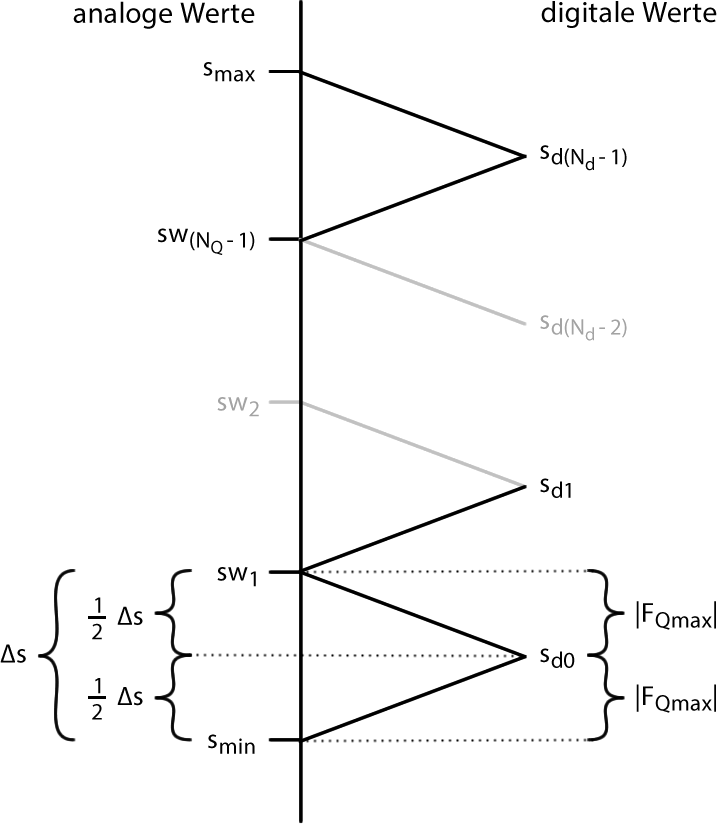
\includegraphics[width=0.8\textwidth]{AD-Wandl_unvollst_Sig-Umf_ohne_delta.png}
	\caption{Analog-Digital-Wandlung mit unvollständigem Signalumfang}
	\label{AD-Wandl_unvollst_Sig-Umf_ohne_delta}
\end{figure}

\subsection{Der technische Unsicherheitsbereich}
Wegen technisch ungenauer Messungen kann ein Wert eines analogen Signals zu hoch oder zu niedrig eingestuft werden. Dies führt zu einer weiteren Fehlerquelle, wenn ein Wert in unmittelbarer Nähe zu einem Schwellwert gemessen wird. Dementsprechend wird dieser Wert entweder einem zu hohen oder zu niedrigen digitalen Wert zugeordnet. Der Bereich um einen Schwellwert herum, in dem solche kritischen Werte gemessen werden können, wird Unsicherheitsbereich $\delta$ genannt. Abbildung \ref{AD-Wandl_vollst_Sig-Umf_mit_delta} veranschaulicht diesen Sachverhalt.

Für den tatsächlichen maximalen Fehler\footnote{Prof.Gemmar benennt den maximalen Fehler mit $F'_{Qmax}$.} $F_{max}$ muss also die Hälfte des Unsicherheitsbereiches zum Quantisierungsfehler addiert werden. Es folgt:
\[
	F_{max} = F_{Qmax} \pm \frac{1}{2} \delta
\]

\begin{figure}[htbp] % positioning htbp: h = here; t = top; b bottom; p own page
	\centering
	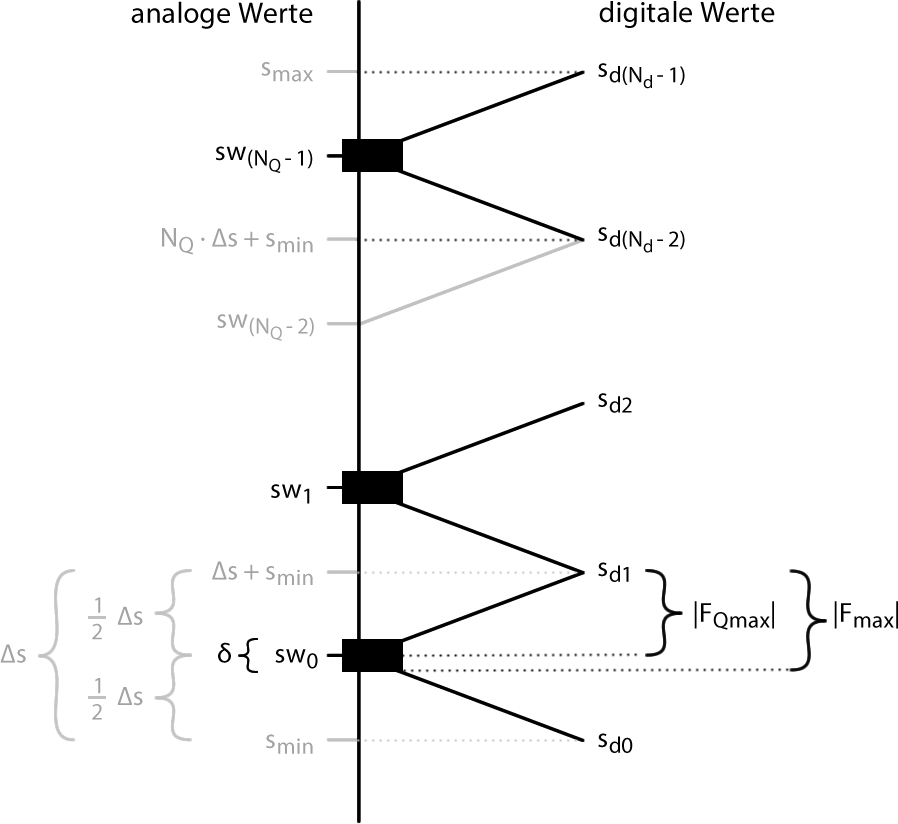
\includegraphics[width=0.8\textwidth]{AD-Wandl_vollst_Sig-Umf_mit_delta.png}
	\caption{technischer Unsicherheitsbereich $\delta$ um die Schwellwerte}
	\label{AD-Wandl_vollst_Sig-Umf_mit_delta}
\end{figure}

%\chapter{Digitale Signale und Zahlensysteme}
%Im folgenden Kapitel geht es um Zahlensysteme und binäre Signale, welche über das Duale Zahlensystem mathematisch erfasst werden können. Ein Binäres Signal ist ein digitales Signal dessen Wertemenge genau zwei Werte besitzt. Beispiele für binäre Mengen sind:
%\[
%	\{0, 1\}; \{wahr, falsch\}; \{high, low\}
%\]

\chapter{Zahlensysteme}
Im folgenden werden Polyadische Zahlensysteme besprochen. Solche Systeme haben die Eigenschaft Zahlen anhand einer Basis in Vielfachen von Potenzen dieser Basis aufzuteilen. Dies erleichtert Operationen auf Zahlen und lässt sich mittels der Potenzschreibweise auch leicht und relativ verständlich aufschreiben. Im Alltag benutzen wir das 10ner Polyadische Zahlensystem mit der Stellenschreibweise.

Ein Beispiel: Die Zahl $7645$ ist in Stellenschreibweise im 10ner System geschrieben. Die Zahl hat die Wertigkeit 5 Einer, 4 Zehner, 6 Hunderter und 7 Tausender. Das selbe dargestellt als Addition von Vielfachen von Potenzen über die Basis 10:
\[
	7645 = 7 \cdot 10^3 + 6 \cdot 10^2 + 4 \cdot 10^1 + 5 \cdot 10^0
\]

Gebrochene Zahlen können mittels Nachkommastellen dargestellt werden. Jede Nachkommastelle steht dann für die Potenz eines Anteils einer Einheit.

Ein Beispiel: Die Zahl $10,23$ ist in Stellenschreibweise im 10ner System geschrieben. Die Zahl hat die Wertigkeit ein Zehner, null einer, zwei zehntel und drei hundertstel. Das selbe dargestellt als Addition von Vielfachen von Potenzen über die Basis 10:
\[
	10,23 = 1 \cdot 10^1 + 0 \cdot 10^0 + 2 \cdot 10^{-1} + 3 \cdot 10^{-2} 
	= 1 \cdot 10^1 + 0 \cdot 10^0 + 2 \cdot \frac{1}{10^1} + 3 \cdot  \frac{1}{10^2}
\]

Eine Ziffer steht also je nach Stelle, an der sie steht, für ein Vielfaches einer Potenz der Basis. Die Potenz wird durch die Stelle bestimmt an der die Ziffer steht. Das Vielfache der Potenz wird mit dem Symbol der Ziffer bestimmt. Da die Wertigkeit einer Potenz grundsätzlich in die jeweils nächste Stelle übertragen wird, gilt für den Wertebereich einer Ziffer $z$ in Basis $B$:
\[
	M_z = \{ z \in \mathbb{N} \mid 0 \le z \le B - 1 \}
\]

Im Allgemeinen kann die Wertigkeit einer ganzen Zahl $Z$ mit $n$ Vorkomma-, $m$ Nachkommastellen und den Ziffern $z_i$ in der Basis $B$ folgendermaßen bestimmt werden:
\begin{eqnarray*}
	Z_B & = & \sum_{i=-m}^n B^i \\
		& = & z_{n-1} \cdot B^{n-1} + z_{n-2} \cdot B^{n-2} + ... 
		+ z_1 \cdot B^1 + z_0 \cdot B^0 + z_{-1} \cdot B^{-1} 
		+ ... + z_{-m} \cdot B^{-m}
\end{eqnarray*}

\section{Zählfunktion}
\label{Zählfunktion} 
Über die Zählfunktion werden Arithmetische Operationen vereinfacht. Wird der Wertebereich einer Ziffer um eins überschritten wird die Ziffer auf $0$ gesetzt und ein Übertrag\footnote{engl. carry} auf die nächste Stelle übernommen. Bei Unterschreiten des Wertebereichs um eins erfolgt eine Anleihe\footnote{engl. borrow} auf die nächst höhere Stelle. Die Ausführung von arithmetischen Operationen lässt sich auf die Zählfunktion zurück führen. Die Berechnung für jede Stelle ist auf einen simplen Algorithmus zurückführbar und somit gut für eine automatische Ausführung geeignet.

\section{Stellenverschiebung}
\label{stellenverschiebung}
Eine weitere Besonderheit ist die Operation der Stellenverschiebung. Eine Stellenverschiebung nach links in einem $B$-System bedeutet eine Division durch $B$ der Zahl. Dies kann bei ganzen Zahlen entweder durch streichen der niedrigsten Stelle geschehen oder bei gebrochenen Zahlen durch verschieben des Kommas nach links. Eine Stellenverschiebung nach rechts bedeutet eine Multiplikation mit $B$ der Zahl. Eine $k$-fache Verschiebung bedeutet eine Division bzw. Multiplikation um die $k$te Potenz der Basis. Beispiele:
\begin{itemize}
	\item
	$1337_{10} \div 10^1 = 133_{10}$
	
	\item 
	$32,1_{10} \cdot 10^2 = 3210_{10}$
	
	\item
	$10110_2 \div 2^1 = 1011_2$
	
	\item
	$111_2 \cdot 2^3 = 111000_2$
\end{itemize}


\section{Stellen- und Ziffernaufwand}
Der Stellen- und Ziffernaufwand einer Zahl ist von der gewählten Basis und der Größe der Zahl abhängig. Wieviele unterschiedliche Zahlen $N$ bei angegebener Stellenzahl $n$ und Basis $B$ dargestellt werden können lässt sich folgendermaßen berechnen:
$$ 
	N = B^n 
$$

Ist gefragt wieviele Stellen $n$ für $N$ unterschiedliche Zahlen unter Verwendung der Basis $B$ aufzuwenden sind, lässt sich die obige Gleichung folgendermaßen umstellen:
$$
	n = \lceil log_B(N) \rceil
$$

Der Ziffernaufwand gibt an wieviele Zeichen zum Darstellen von einer bestimmten Anzahl unterschiedlicher Zahlen nötig sind. Für jede Stelle sind Anzahl Ziffern in Höhe der Basis notwendig. Der Ziffernaufwand $zn_B$ für $N$ unterschiedliche Zahlen in der Basis $B$ wird also bestimmt mit:
$$
	zn_B = B \cdot n = B \cdot \lceil log_B(N) \rceil
$$

%\section{Das Dualsystem}
%Das Dualsystem von der Komplexität her gesehen das einfachste Zahlensystem. Wegen der Basis $2$ sind nur die Ziffern $0$ und $1$ nötig. Die beiden Ziffern sind direkt-komplementär zueinander. Also können arithmetische Rechenoperationen mit einfachen logischen Funktionen, wie $\wedge$ und $\vee$, realisiert werden.

%Die Wertigkeit einer Dualzahl lässt sich folgendermaßen berechnen:
%$$
%	Z_2 = \sum_{i=0}^n b_i 2^i 
%		\textnormal{ mit } b_i \in \{0, 1\} \wedge i,n \in \mathbb{N}
%$$

%Für die Stellenverschiebung werden auch die englischen Begriffe Left-Shift und Right-Shift verwendet. Ein Left-Shift bewirkt eine Multiplikation mit $2$, ein Right-Shift bewirkt eine Division mit $2$.
%TODO: Vergleich Binärsystem und Zehnersystem im Bezug auf Stellen und Ziffernaufwand einfügen.

\section{Umwandlung von Zahlensystemen}
Mit Hilfe des Hornerschemas lässt sich ein allgemeingültiger Allgorithmus zur Umwandlung eines beliebigen Zahlensystems in ein anderes herleiten. Das Hornerschema beschreibt das sukzessive Ausklammern eines Faktors. Dieses Verfahren lässt sich gut auf die Potenzschreibweise einer Zahl anwenden.

Beispielsweise lässt sich die Zahl 2.938 wie folgt zerlegen:
\begin{eqnarray*}
	2.938 & = & 8 + 10 \cdot 3 + 10^2 \cdot 9 + 10^3 \cdot 2 \\
	& = & 8 + 10 \cdot (3 + 10 \cdot(9 + 10 \cdot 2))
\end{eqnarray*}
Anschließend können die einzelnen Stellen durch Division mit der Basis aquiriert werden indem das jeweilige Ergebnis wiederum mit der Basis dividiert wird.
$$
\begin{array}{rrrl}
  8 + 10 \cdot (3 + 10 \cdot(9 + 10 \cdot 2)) \div 10 & = & 3 + 10 \cdot(9 + 10 \cdot 2)  & \textnormal{Rest } 8 \\
  3 + 10 \cdot(9 + 10 \cdot 2) \div 10 & = & 9 + 10 \cdot 2  & \textnormal{Rest } 3 \\
  9 + 10 \cdot 2 \div 10 & = & 2  & \textnormal{Rest } 9 \\
  2 \div 10 & = & 0  & \textnormal{Rest } 2 \\
\end{array}
$$

Die Zahl $25_{10}$ lässt sich in Potenzschreibweise zur Basis 2 folgendermaßen aufschreiben:
\begin{eqnarray*}
	25_{10} & = & 1 + 2 \cdot 0 + 2^2 \cdot 0 
		+ 2^3 \cdot 1 + 2^4 \cdot 1 \\
	& = & 1 + 2 \cdot (0 + 2 \cdot (0 
		+ 2 \cdot (1 + 2 \cdot 1))) \\
\end{eqnarray*}
Anschließend können wiederum die einzelnen Stellen für die Stellenschreibweise zur Basis $2$ durch wiederholte Division mit der Basis $2$ aquiriert werden.
$$
\begin{array}{rrrl}
	1 + 2 \cdot (0 + 2 \cdot (0 + 2 \cdot (1 + 2 \cdot 1 + ))) \div 2 
		& = & 0 + 2 \cdot (0 + 2 \cdot (1 + 2 \cdot 1)) 
		& \textnormal{Rest } 1\\
		0 + 2 \cdot (0 + 2 \cdot (1 + 2 \cdot 1)) \div 2
		& = & 0 + 2 \cdot (1 + 2 \cdot 1) 
		& \textnormal{Rest } 0\\
		0 + 2 \cdot (1 + 2 \cdot 1) \div 2
		& = & 1 + 2 \cdot 1 
		& \textnormal{Rest } 0\\
		1 + 2 \cdot 1 \div 2
		& = & 1 
		& \textnormal{Rest } 1\\
		1 \div 2
		& = & 0 
		& \textnormal{Rest } 1\\
\end{array}
$$
Da durch das Dividieren mit der Basis immer die niedrigste Stelle des aktuellen Ergebnisses aquiriert wird, ist die letzte Stelle die höchste und muss somit als erstes im Ergebnis notiert werden usw. Das Ergebnis der Umwandlung von $25_{10}$ in das Dualsystem ist also $11001_2$.

Allgemein kann folgender Algorithmus angewandt werden um eine ganze Zahl $Z_B$ zur Basis $B$ in die Basis $B^*$ zu wandeln:
\begin{enumerate}
\renewcommand{\labelenumi}{\alph{enumi})}
\item
Teile $Z_B$ durch $B^*$. Notiere das Ergebnis $Z'_B$ und den Rest. 

\item
Wiederhole Schritt a mit $Z'_B$ statt $Z_B$ bis das Ergebnis aus Schritt a $0$ ist.

\item
Notiere die Zahl im $B^*$-System. Der Rest der letzten Division ist die höchste Stelle der Zahl im $B^*$-System. Der Rest der vorletzten Division ist die zweit-höchste Stelle der Zahl im $B^*$-System usw.
\end{enumerate}

Für die Umwandlung echt-gebrochener Zahlen lässt sich ein ähnliches Verfahren anwenden. Hierbei muss die Zahl wiederholt mit der neuen Basis multipliziert werden. Nach jeder Multiplikation wird der Vorkommaanteil notiert. Mit dem Nachkommaanteil wird die Multiplikation fortgesetzt solange bis der Nachkommaanteil $0$ ergibt oder der gleiche Vorkommaanteil, wie zuvor, erreicht wird. Im letzten Fall ergibts sich daraus die Periode. Die Periode lässt sich ab der Stelle mit der Ziffer, die später erneut gefunden wurde, bis zu der Stelle mit der gleichen Ziffer genau feststellen, da sich ab dieser Stelle die vorhergehenden Rechnungen wiederholen würden.

Beispielsweise lässt sich die Zahl $0,375_{10}$ in Potenzschreibweise zur Basis 2 wie folgt zerlegen:
\begin{eqnarray*}
0,375_{10} & = & 2^{-1} \cdot 0 + 2^{-2} \cdot 1 + 2^{-3} \cdot 1 \\
& = & 2^{-1} \cdot (0 + 2^{-1} \cdot (1 + 2^{-1} \cdot 1))
\end{eqnarray*}
Die einzelnen Stellen zur Basis 2 erhält man, indem mit 2 multipliziert wird. Die Resultierende Vorkommastelle ist die erste Stelle. Der Nachkommaanteil wird erneut mit 2 multipliziert um die nächste Stelle zu erhalten.
$$
\begin{array}{rrl}
	2^{-1} \cdot (0 + 2^{-1} \cdot (1 + 2^{-1} \cdot 1)) \cdot 2 
	& = & 
	\underbrace{0}_{Vorkommaanteil} + \underbrace{2^{-1} \cdot (1 + 2^{-1} \cdot 1)}_{Nachkommaanteil} \\
	
	2^{-1} \cdot (1 + 2^{-1} \cdot 1) \cdot 2 
	& = & 
	\underbrace{1}_{Vorkommaanteil} 
	+ \underbrace{ 2^{-1} \cdot 1 }_{Nachkommaanteil}\\
	
	2^{-1} \cdot 1
	\cdot 2 & = & 
	\underbrace{1}_{Vorkommaanteil} \\
\end{array}
$$
Da durch das Multiplizieren mit der Basis immer die höchste Stelle des aktuellen Ergebnisses aquiriert wird, ist die erste Stelle die höchste und muss somit als erstes im Ergebnis notiert werden usw. Das Ergebnis der Umwandlung von $0,375_{10}$ in das Dualsystem ist also $0,011_2$.

Ein Beispiel mit Periode: die Zahl $0,1_{10}$ soll in das Binärsystem gewandelt werden.
$$
\left|
\begin{array} {rrl}
	0,1 \cdot 2 &=& 0,2 \\
	0,2 \cdot 2 &=& 0,4 \\
	0,4 \cdot 2 &=& 0,8 \\
	0,8 \cdot 2 &=& 1,6 \\
	0,6 \cdot 2 &=& 1,2 \\
\end{array}
\right|
$$
$$
\begin{array} {rrl}
	0,2 \cdot 2 &=& 0,4 \\
\end{array}
$$
Das Ergebnis ist $0,1_{10} \mapsto 0,\overline{00011}_2$ \\
Ein weiteres Beispiel: $0,2_{10} \mapsto 0,\overline{00111}_2$

Zahlen mit ganzem und gebrochenem Teil werden gewandelt in dem der ganze Teil mit dem Divisionsverfahren und der gebrochene Teil mit dem Multiplikationsverfahren gewandelt wird. Die Ergebnisse der beiden Teilschritte ergeben durch Komma getrennt das Gesamtergebnis.

Ein Beispiel: $19,625_{10}$ soll in das Dualzahlsystem gewandelt werden.
\begin{itemize}
\item
	Wandlung des ganzen Teils:
	$$ \begin{array}{rrrl}
		19 \div 2 & = & 9 & \textnormal{Rest } 1 \\
		 9 \div 2 & = & 4 & \textnormal{Rest } 1 \\
		 4 \div 2 & = & 2 & \textnormal{Rest } 0 \\
		 2 \div 2 & = & 1 & \textnormal{Rest } 0 \\
		 1 \div 2 & = & 0 & \textnormal{Rest } 1 \\
	\end{array} $$
	also ist der ganze Teil $19_{10} \mapsto 10011_2$
\item
	Wandlung des gebrochenen Teils:
	$$ \begin{array}{rrrl}
		0,625 \cdot 2 & = & 1,25 \\
		 0,25 \cdot 2 & = & 0,5  \\
		  0,5 \cdot 2 & = & 1,0  \\
	\end{array} $$
	also ist der gebrochene Teil $0,625_{10} \mapsto 0,101_2$
\item
	Das Ergebnis ist demnach  $19,625_{10} \mapsto 10011,101_2$ 
\end{itemize}

\subsection{Zahlenwandlungen mit Basen der Form $2^i$}
Die fortgesetzte Division ist bei der Wandlung vom Dualsystem in ein anderes $2^i$-System durch einfache Stellenverschiebung um $i$ möglich. Der Rest sind dabei die Stellen, welche durch die Verschiebung wegfallen.

Beispielsweise lässt sich die Zahl $1010100110_2$ durch Tetradenanordnung leicht in das Hexadezimalsystem\footnote{Hexa = 6; dezi = 10; 16ner System; $16 = 2^4$} wandeln:
$$
\begin{array}{rrrl}
	10\hspace{1mm}1010\hspace{1mm}0110_2 \div 16 & = & 10\hspace{1mm}1010 
		& \textnormal{ Rest } 0110_2 = 6_{16} \\
	10\hspace{1mm}1010_2 \div 16 & = & 10 
		& \textnormal{ Rest } 1010_2 = A_{16} \\
	10_2 \div 16 & = & 0 
		& \textnormal{ Rest } 10_2 = 2_{16} \\
\end{array}
$$
$$
	\underbrace{10}_{2} \underbrace{1010}_{A} \underbrace{0110}_{6}
$$
$$
	10\hspace{1mm}1010\hspace{1mm}0110_2 \mapsto 2A6_{16}
$$

Mit der Umkehrfunktion lässt sich die Hexadezimaldarstellung einer Zahl auch in die Dualdarstellung wandeln, indem jede Stelle in vier bits codiert wird. Allgemein kann von vom $2^i$-System in das Binärsystem gewandelt werden, indem jeweils eine Stelle der Zahl im $2^i$-System in $i$~Stellen des Binärsystems gewandelt werden. Ein Beispiel:
$$
	\underbrace{A}_{1010} \underbrace{F}_{1111} \underbrace{F}_{1111} \underbrace{E}_{1110}
$$
$$
	AFFE_{16} \mapsto 1010\hspace{1mm}1111\hspace{1mm}1111\hspace{1mm}1110_2
$$

\begin{center}
Weitere Beispiele:
\end{center}
$$ 1\hspace{1mm}00\hspace{1mm}10\hspace{1mm}00_2 \mapsto 1020_4 $$
$$ 231_4 \mapsto 10\hspace{1mm}11\hspace{1mm}01_2 $$
$$ 1\hspace{1mm}001\hspace{1mm}000_2 \mapsto 110_8 $$
$$ 55_8 \mapsto 101\hspace{1mm}101_2 $$

\subsection{Umgang mit Perioden}
Je nach Zahlensystem können Zahlen nur mit Periode in Stellenschreibweise geschrieben werden. Die Zahlen können in einen Bruch gewandelt werden. Im Folgenden werden die mathematischen Zusammenhänge erklärt.

Sei $p$ eine periodische Zahl ohne Vorperiode in einem beliebigen Zahlensystem zur Basis $B$ und $n$ sei deren Periodenlänge. Sei $o$ eine ganze Zahl ohne Periode und wie folgt definiert:
$$
	o = \underbrace{\underbrace{p \cdot B^n}_\textnormal{Periode als ganzzahliger Anteil} - p}_\textnormal{Periode subtrahiert}
$$
$o$ ist also die Darstellung der Periode als Ganzzahl. Durch Umformung gilt:
\begin{eqnarray*}
	o & = & p \cdot B^n - p \\
	o & = & (B^n - 1) \cdot p \\
	p & = & \frac{o}{B^n - 1}\\	
\end{eqnarray*}
Beispiel: $0,\overline{1011}_2$ soll in einen Bruch zur Basis $10$ gewandelt werden.
$$ o = 1011_2; n = 4; B = 2 $$
\begin{eqnarray*}
	0,\overline{1011}_2 & \mapsto & \frac{1011_2}{2^4 - 1} \\
	0,\overline{1011}_2 & \mapsto & \frac{11_{10}}{15_{10}}
\end{eqnarray*}

Bei einer Zahl mit Vorperiode der Länge $k$ muss zuerst die Vorperiode durch Multiplizieren mit $B^k$ eliminiert werden. Danach lässt sich der Periodische Anteil berechnen, wie oben angegeben. Das Resultat muss um die Operation auszugleichen mit $\frac{1}{B^k}$ multipliziert und die Vorperiode als Bruch addiert werden. Ein Beispiel: Wandlung der Zahl $0,01\overline{01001011}_2$ in einen Bruch im Dezimalsystem.
\begin{enumerate}
\item
	Eliminiere Vorperiode
	$$ 0,01\overline{01001011}_2 = 0,01 
		+ \frac{1}{2^2} \cdot 0,\overline{01001011}_2$$

\item
	Wandle periodischen Anteil in Bruch um
	$$ 0,01\overline{01001011}_2 = 0,01_2 
		+ \frac{1}{2^2} \cdot \frac{01001011_2}{2^8 - 1}$$
		
\item
	Berechne Ergebnis
	$$ 0,01\overline{01001011}_2 = \frac{1}{4} 
		+ \frac{1}{4} \cdot \frac{75}{255} = \frac{11}{34}$$
\end{enumerate}

Mit der Formel $p = \frac{o}{B^n - 1}$ lassen sich auch manche Brüche in Stellenschreibweise umformen. Zum Beispiel kann $\frac{1}{3}$ auch anders geschrieben werden als $\frac{1}{2^2 - 1}$. Mit Hilfe der Formel kann die Periodenlänge $n = 2$, die Periode als Ganzzahl $o = 1$ und die neue Basis $B = 2$ bestimmt werden. Also ist $\frac{1}{3} \mapsto 0,\overline{01}_2$ .
Ist eine Zahl mit Periode auf diese Weise bestimmt, lassen sich Vielfache zur Basis $B$ der Zahl ebenfalls bestimmen indem die Periodischen Stellen geschoben werden. Beispielsweise ist $ \frac{1}{6} \mapsto 0,0 \overline{01}_2 $ , da $\frac{1}{3} \mapsto 0, \overline{01} $ und $ \frac{1}{3} \cdot 2^{-1} = \frac{1}{6}$ ist. Die Multiplikation mit $2^{-1}$ kann durch eine Stellenverschiebung der Stellen einer Dualzahl um eine Stelle nach rechts vollzogen werden.\footnote{siehe Abschnitt \ref{stellenverschiebung} zum Thema Stellenverschiebung}  

\section{Addition und Subtraktion im Dualsystem}
Nach der Zählfunktion\footnote{Siehe Abschnitt \ref{Zählfunktion} unter Zählfunktion} gelten folgende Regeln:
\begin{eqnarray*}
	0 + 0 & = & 0 \\
	0 + 1 & = & 1 \\
	1 + 0 & = & 1 \\
	1 + 1 & = & 0 +\textnormal{ carry in die nächsthöhere Stelle}\\ 
	\\
	0 - 0 & = & 0 \\
	0 - 1 & = & 1 -\textnormal{ borrow von der nächsthöheren Stelle}\\
	1 - 0 & = & 1 \\
	1 - 1 & = & 0 \\ 
\end{eqnarray*}

Beim schriftlichen Addieren von Dualzahlen kann folgendes Verfahren angewandt werden:
\begin{enumerate}
\item
	Zähle die 1en in der ersten Spalte.
\item
	die erste Stelle der Anzahl 1en als Dualzahl wird in dieselbe Spalte geschrieben. Die nachfolgenden Stellen werden in die jeweils nachfolgenden Spalten als carry übernommen.
\item
	Wiederhole Schritt 1. mit den nachfolgenden Spalten.
\end{enumerate}

Beispiel:

\begin{tabular}{lrrrrr}
  & 1 & 0 & 0 & 1 & 1 \\
+ & 0 & 1 & 0 & 1 & 1 \\
\hline
  &   &   &   & 1 &   \\
  &   &   & 1 &   &   \\
\hline
  & 1 & 1 & 1 & 1 & 0
\end{tabular}

\subsection{Subtraktion durch Komplementaddition}
Das Basis-Komplement $K_B(Z)$ einer Zahl $Z$ mit Anzahl Stellen $n$ ist definiert mit:
$$ K_B(Z) = B^n - Z$$

Das Basis-Komplement ist die Umkehrfunktion von sich selbst.
\begin{eqnarray*}
K_B(K_B(Z)) &=& K(B^n - Z) \\
&=& B^n - (B^n - Z) \\
K_B(K_B(Z)) &=& Z \\
\end{eqnarray*}

Das Stellenkomplement\footnote{Das Stellenkomplement wird auch Einerkomplement genannt.} $K'_B(Z)$ ist definiert über die Differenz jeder Ziffer an jeder Stelle zur höchstwertigen Ziffer. Es gilt also für jede Ziffer $z_i$ an Stelle $i$:
$$ K'_B(Z): z_i \mapsto ((B - 1) - z_i) $$

Das Basis-Komplement lässt sich leicht berechnen indem das Stellenkomplement um eins inkrementiert wird. Beispiel:
$$ K_{10}'(123) = 876 $$
$$ K_{10}(123) = 1000 - 123 = 876 + 1 = 877 $$

Werden negative Zahlen mit dem Basis-Komplement dargestellt, kann die Subtraktion zweier Zahlen über die Addition der beiden Zahlen abgearbeitet werden. Dies gilt weil:
$$
  a - b = a + K(b) - B^n = a - b + B^n - B^n
$$
Das Subtrahieren von $B^n$ kann methodisch je nach Fall behandelt werden. Ist der Minuend größer oder gleich dem Subtrahenden \marginpar{$M \ge S$} wird die führende eins nach der Berechnung gestrichen. Wichtig bei dieser Methode ist, dass Minuend und Subtrahend die gleiche Stellenanzahl besitzen. Die höheren Stellen des Subtrahenden müssen gegebenenfalls mit Nullen aufgefüllt werden und über diese Zahl das Komplement gebildet werden. Beispiel:
\begin{eqnarray*}
	8127_{10} - 342_{10} & = & 8127 - 0342                  \\
	                     & = & 8127 + K_{10}(0342) - 10000  \\
	                     & = & 8127 + 10000 - 0342 - 10000  \\
	                     & = & 8127 + 9658 - 10000  \\                
\end{eqnarray*}
Addition von 8127 und 9658. Die Subtraktion von 10000 erfolgt über das Streichen der führenden 10000der-Stelle.
\begin{center}
\begin{tabular}{lrrrr}
  & 8 & 1 & 2 & 7 \\
+ & 9 & 6 & 5 & 8 \\
\hline
  &   &   & 1 &   \\
\textit{1} &   &   &   &   \\
\hline
  & 7 & 7 & 8 & 5
\end{tabular}
\end{center}

Ist der Minuend kleiner als der Subtrahend \marginpar{$M < S$} steht das Ergebnis im negativen Basis-Komplement. Das Ergebnis kann also über das Komplement des Zwischenergebnisses berechnet werden. Beispiel:
\begin{eqnarray*}
	342_{10} - 8127_{10} & = & 342 + K_{10}(8127) - 10000  \\
	                     & = & 342 + 10000 - 8127 - 10000  \\
	                     & = & 342 + 1873 - 10000          \\
	                     & = & 2215 - 10000                \\
	                     & = & -(10000 - 2215)             \\
	                     & = & -K_{10}(2215)               \\
	                     & = & -7785                       \\
\end{eqnarray*}

Die angegbenen Methoden lassen sich auf jedes Basis-System anwenden. \\ Beispiel: $65_{10} - 23_{10} = 42_{10} \mapsto 1000001_2 - 10111_2 = 101010_2$ \\
\begin{center}
\begin{tabular}{lr|lr}
dezimal                           &      & dual             &                                 \\ \hline
                                  &  65  &                  &                       100 0001  \\
$K_{10}(23)$ &           \underline{+77} & $K_2(001 0111)$  &           \underline{+110 1001} \\
             & \underline{ \textit{1}42} &                  & \underline{ \textit{1}010 1010} \\
             &              \textbf{+42} &                  &               \textbf{+10 1010} \\
\end{tabular}
\end{center}
Beispiel: $12_{10} - 74_{10} = -62_{10} \mapsto 1100_2 - 100 1010_2 = -11 1110_2$
\begin{center}
\begin{tabular}{lr|lr}
dezimal       &                           & dual              &                                 \\ \hline
              &                       12  &                   &                       000 1100  \\
$K_{10}(74)$  &           \underline{+26} & $K_2(100 1010)$   &           \underline{+011 0110} \\
              & \underline{ \textit{0}38} &                   & \underline{ \textit{0}100 0010} \\
$-K_{10}(38)$ &              \textbf{-62} & $-K_2(100 0010)$  &               \textbf{-11 1110} \\
\end{tabular}
\end{center}

%TODO Abschnitt zu Multiplikation und Division von Dualzahlen ergänzen

\section{Darstellung und Arithmetik rationaler Zahlen}
In der Praxis gibt es in digitalen automatischen Rechenanlagen zwei Darstellungsarten für rationale Zahlen: das Festkommaformat und das Fließkommaformat. Den folgenden zwei Abschnitten wird näher auf die einzelnen Formate eingegangen.

\subsection{Festkommma-Arithmetik}
Die Festkommadarstellung wird verwendet um Zahlen Z im Wertebereich $W_F = \{ Z~\in~\mathbb{Q} \mid -1 < Z < 1\}$ abzubilden. Das höchstwertige Bit wird als Vorzeichenbit \textit{VZ} verwendet und gibt das Vorzeichen der Zahl an. Die übrigen Bits werden als Mantissenbits verwendet. Die Mantisse gibt alle Nachkommastellen an. Die Vorkommastelle ist immer null und muss deshalb nicht codiert werden. Abbildung \ref{Festkommadarstellung} zeigt Schematisch die Festkommadarstellung.

\begin{figure}[htbp] % positioning htbp: h = here; t = top; b bottom; p own page
	\centering
	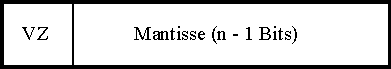
\includegraphics{Festkommaarithmetik.pdf}
	\caption{Festkommadarstellung einer Zahl}
	\label{Festkommadarstellung}
\end{figure}

Der numerisch kleinste Abstand zwischen zweier Zahlen ist konstant $\Delta Z = 2^{n-1}$. Dies ist ein äquidistantes Zahlenformat.

Der größte Zahlenwert $Z_{max}$ beträgt:
\begin{eqnarray*}
Z_{max} &=& 0,111...1              \\
        &=& \sum_{i=1}^{n-1}2^{-i} \\
        &=& 1 - 2^{-(n-1)}
\end{eqnarray*}

Der kleinste Zahlenwert $Z_{min}$ beträgt:
\begin{eqnarray*}
Z_{min} &=& -0,111...1              \\
        &=& -\sum_{i=1}^{n-1}2^{-i} \\
        &=& -1 + 2^{-(n-1)}
\end{eqnarray*}

\subsection{Fließkomma-Arithmetik}
Bei der Fließkommadarstellung wird zusätzlich ein Exponent zur Mantisse  gespeichert. Dem Exponenten wird ein konstanter Wert implizit hinzu addiert um auf ein Vorzeichenbit für den Exponenten verzichten zu können. Die so entstandene Zahl wird Charakteristik einer Fließkommazahl genannt. Abbildung \ref{Fliesskommadarstellung} zeigt schematisch die Fließkommadarstellung.
\begin{figure}[htbp] % positioning htbp: h = here; t = top; b bottom; p own page
	\centering
	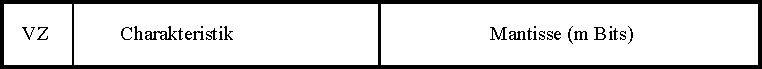
\includegraphics{Fliesskommaarithmetik.pdf}
	\caption{Fließkommadarstellung einer Zahl}
	\label{Fliesskommadarstellung}
\end{figure}

Der Wert einer dualen Fließkommazahl $Z$ mit Mantisse $M$, Charakteristik $C$ mit konstantem Teil $k$ und Vorzeichen $VZ$ lässt sich also berechnen mit:
$$ Z = VZ \cdot M \cdot 2^{C-k} $$

Fließkommazahlen werden normalisiert. Das heißt der Exponent wird so gewählt, dass die Mantisse genau eine Vorkommastelle mit einer Wertigkeit größer null hat. Bei Dualzahlen im Fließkommaformat ist die Vorkommastelle deshalb immer eins und muss nicht gespeichert werden. Eine Ausnahme ist hier die Null. Null hat auch als Vorkommastelle die Ziffer 0 und die Nachkommastellen sind bekanntlicher Weise ebenfalls Null. Deshalb wird die Konvention eingeführt, dass wenn alle Ziffern der dualen Fließkommazahl null sind, der Wert Null gemeint ist.

Beispiel: $+0,010100111_2$ im IEEE 754 32bit float Format:
\begin{center}
\begin{tabular}{ccc}
VZ & Charakteristik (8bit; $k = 2^{8-1}-1$) & Mantisse (23bit) \\
 + & E + k = -2 + 127 = 125 & 1,0100\hspace{1mm}111 \\
 0 & 0111 1101   & 0100 1110 0000 0000 0000 000
\end{tabular}
\end{center}

Vor der Addition oder Subtraktion zweier Fließkommazahlen müssen diese erst denormalisiert werden. Der niedrigere Exponent wird immer auf den höherwertigen aufgewertet und die Mantisse um eben so viele Stellen nach rechts verschoben. Durch dieses Verfahren können zwangsläufig Rechenfehler entstehen, da im Computer bei der Denormalisierung bzw. Normalisierung signifikante Stellen der Mantisse verloren gehen können. Beispiele:
\begin{eqnarray*}
1,0101E3 + 1,1110111E0 &=& 1,0101E3 + 0,0011110111E3 \\
&=& (1,0101 + 0,0011110111)E3 \\
&=& 1,100011011E3 \\
\end{eqnarray*}
\begin{eqnarray*}
1,1101E2 - 1,01E1 &=& 1,1101E2 - 0,101E2 \\
&=& (1,1101 - 0,101)E2 \\
&=& 1,0011E2 \\
\end{eqnarray*}

Nach einer Multiplikation oder einer Division muss das Ergebnis häufig normalisiert werden. Dabei können wiederum zwangsläufig Rechenfehlehler entstehen.
%TODO Beispiele zur Multiplikation und Division einfügen

\chapter{Codes}
Nachrichten werden in Form von Zeichenketten dargestellt. Zeichenketten wiederum bestehen aus einzelnen Zeichen. Die Zeichen, die für bestimmte Nachrichten verwendet werden, werden im jeweiligen Alphabet\footnote{Ein Alphabet wird auch Zeichenvorrat genannt.} festgelegt. Welche Zeichenketten ein Wort einer Nachricht bilden und welche nicht wird in den Produktionsregeln festgelegt.

Ein Wort kann über Konkatenation\footnote{Konkatenation ist die Aneinanderreihung von Zeichen} von Zeichen gebildet werden. Das Symbol der Konkatenation ist "`$\circ$"'. Wörter einer bestimmten Länge über ein Alphabet werden in Wortmengen zusammen gefasst. Hierzu wird das Alphabetssymbol mit der im Exponenten angegebenen Wortlänge angegeben.
Beispiel: \\
Es sei das Alphabet $A = \{0, 1\}$. \\
Die Zeichen 0 und 1 sind Elemente von Alphabet $A$. Kurz: $0,1 \in A$ \\
Ein Wort über $A$ ist $w = 0 \circ 1 \circ 1 \circ 0 = 0110$ \\
$w$ ist Element von $A^4$. Kurz: $w \in A^4$ \\

In der Praxis ist das zu verarbeitende Alphabet oft länger als das technisch verfügbare Alphabet. Der Computer kennt auf unterster Ebene nur zwei unterschiedliche Zeichen. Dem Computer steht also ein binäres Alphabet zur Verfügung. Um dennoch umfangreichere Alphabete und Nachrichten, die über dieses gebildet werden, verarbeiten zu können, müssen die Zeichen des Ursprungsalphabets auf Wörter des kleineren Alphabets abgebildet werden. Dieser Umsetzungsprozess wird Codierung genannt. Ein Code $c$ ist also aus dieser Sicht eine eindeutige Zuordnung zwischen Zeichen aus einem Urspungsalphabet $U$ auf Wörter eines anderen Alphabets $A$.
$$c: U \mapsto A^m$$
$$c: u_i \mapsto a_1a_2...a_m 
	\textnormal{ mit } u_i \in U \wedge a_i \in A$$

Mit einem Alphabet $A$ und $m$ vielen Stellen können maximal $|A|^m$ viele Zeichen codiert werden. Um den minimalen Stellenaufwand $S_{min}$ für $n$ unterschiedliche Zeichen zu bestimmen gilt demnach:
$$ S_{min} = \lceil log_{|A|}(n) \rceil $$

Im Folgenden wird beispielhaft berechnet wieviele Bits mindestens nötig sind um die Dezimalziffern $\{0,1,2, ... , 9\}$ zu codieren.
$$S_{min} = \lceil ld(10) \rceil = 4$$
Demnach werden mindestens vier bit benötigt um zehn Zeichen über das Binäralphabet abzubilden. Mit vier bit wären allerdings $2^4 = 16$ unterschiedliche Konkatenationen von Zeichen möglich. Um irgendeine Zuordnung von Binärworten auf die zehn Ziffern zu definieren gibt es 
$$ \frac{16!}{(16 - 10)!} \approx 2,9 \cdot 10^{10} \textnormal{ Möglichkeiten} $$
Tatsächlich Verwendung finden nur wenige. Welche Vorteile welche Abbildung bringt, wird in den nachfolgenden Abschnitten besprochen.

\section{Beschreibungsmerkmale für Codes}
Grundsätzlich wird zwischen Alphanumerischen Codes und Numerischen Codes unterschieden. Alphanumerische Codes dienen der Darstellung von Ziffern und anderen Zeichen, wie Buchstaben, Trenn und Sonderzeichen und weitere. Numerische Codes dienen der Darstellung von Zahlen. Numerische Codes lassen sich in Wortcodes und Zifferncodes unterteilen. Bei Zifferncodes wird, wie bei Alphanumerischen Codes, jede Ziffer einzeln codiert. In Wortcodes wird dagegen eine Zahl als Ganzes codiert. Ein Beispiel dafür ist der Dualzahlencode. Der Nachteil dabei ist der Kodieraufwand bei der Wandlung bei der Ein-, Ausgabe. Der Vorteil dabei ist, dass arithmetische Operationen oft direkt möglich sind.

Allgemeine Beschreibungsmerkmale für Codes sind:
\begin{itemize}
\item
	Die \textbf{Bewertbarkeit $W$:} Für jede Stelle $i$ in einem Codewort wird eine  Stellenwertigkeit $w_i$ definiert. Der Dualzahlencode ist zum Beispiel bewertet.
\item
	Das \textbf{Gewicht $G$} ist die Anzahl der mit 1en belegten Stellen in einem Codewort. Bei einem gleichgewichteten Code haben alle Codewörter das gleiche Gewicht.
\item
	Die \textbf{Distanz $D$} zweier Codewörter ist die Anzahl stellen in denen sich die Codewörter unterscheiden.
\item
	Die \textbf{Hamming Distanz $HD$} ist die minimale Stellendistanz zwischen beliebigen Codewörtern eines Codes.
	$$HD(C) = min(D(cw_a, cw_b)) \textnormal{ mit } cw_a, cw_b \in C 
		\wedge cw_a \ne cw_b $$
\item
	Die \textbf{Stetigkeit}: ein Code ist stetig, wenn die Distanz zwischen benachbarten Codewörtern im gesamten Code gleich ist.
	$$ C \textnormal{ ist stetig} \Leftrightarrow D(cw_i, cw_{i+1}) = D(cw_j, cw_{j+1}) $$
\item
	Die \textbf{Redundanz}: ein Code ist redundant, wenn mögliche Kombinationen von Zeichen nicht als Codewörter genutzt werden.
\item
	Die \textbf{absolute Redundanz\footnote{Differenz zwischen Anzahl benötigten Bits für alle Kombinationen und Anzahl verwendeten Bits} $R_a$} ist eine Kenngröße eines Codes. Die absolute Redundanz wird über die Anzahl der Kombinationsmöglichkeiten $N$ und die Anzahl Codewörter $N_{cw}$ berechnet. Die Anzahl Kombinationsmöglichkeiten hängt von der Wortlänge $len_{cw}$ des Codes ab. Es gilt:
	$$ N = 2^{len_{cw}} $$
	$$ R_a = ld(N) - ld(N_{cw}) \textnormal{ [bit]} $$
	Beispiel: Redundanz des BCD-Codes für die Ziffern 0 bis 9
	$$ N = 2^4 $$
	$$ N_{cw} = 10 $$
	$$ R_a = ld(2^4) - ld(10) \approx 4 - 3,32 = 0,68 Bit $$
\item
	Die \textbf{relative Redundanz\footnote{Verhältnis zwischen nicht benutzten bits zu insgesamt verwendeten bits} $R_r$} ist eine Kenngröße eines Codes. Die relative Redundanz wird über die Anzahl der Kombinationsmöglichkeiten $N$ und die absolute Redundanz berechnet. Es gilt:
	$$ R_r = \frac{R_a}{ld(N)} $$
\item
	Die \textbf{Vollständigkeit:} Ein Code wird vollständig genannt wenn die absolute Redundanz null ist. Ist die absolute Redundanz größer null, wird der Code als unvollständig bezeichnet.
	$$ C \textnormal{ ist vollständig} \Leftrightarrow R_a = 0 $$
	$$ C \textnormal{ ist unvollständig} \Leftrightarrow R_a > 0 $$
\item
	\textbf{binär-reflektierend:} Ein Code ist binär-reflektierend, wenn die Codewörter aus der Hälfte des Codes gleich der Codewörter der anderen Hälfte des Codes sind mit Ausnahme der vordersten Stelle, die mit jeweils 0 bzw. 1 codiert ist.
\item
	\textbf{selbstkomplementierend / selbstinvertierend:} Ein Code ist selbstkomplementierend, wenn das Neuenerkomplement des Dezimalwertes identisch mit dem Stellenkomplement des jeweiligen Codewortes des Dezimalwertes ist.
\item
	\textbf{prüfbar bzw. gesichert:} Ein Code ist prüfbar, wenn eine Fehlererkennung möglich ist. Dies ist nur mit redundanten Codes möglich. Ausführlich wird dies im Abschnitt \ref{gesicherte_codes} besprochen.
\item
	\textbf{fehlerkorrigierbar:} Ein Code ist fehlerkorrigierbar, wenn eine Fehlererkennung möglich ist und Fehler korrigiert werden können. Dies ist nur mit redundanten Codes möglich. Ausführlich wird dies im Abschnitt \ref{gesicherte_codes} besprochen.
\end{itemize}

\section{Beispiele für bekannte Ziffern-Codes}
\subsection*{Bewertete Ziffern-Codes}

\begin{minipage}[t]{0.47\textwidth}
	\textbf{8-4-2-1 Code} mit den Eigenschaften:
	\begin{itemize}
	\item
		stetig / einschrittig
	\item
		bewertet 8 - 4 - 2 - 1
	\end{itemize}
	\texttt{
	\begin{tabular}{rl}
	\textnormal{Dezimalziffer} & \textnormal{8-4-2-1 Code} \\ \hline
	0             & 0000         \\
	1             & 0001         \\
	2             & 0010         \\
	3             & 0011         \\
	4             & 0100         \\
	5             & 0101         \\
	6             & 0110         \\
	7             & 0111         \\
	8             & 1000         \\
	9             & 1001         \\
	\end{tabular}
	}
\end{minipage}
\hspace{0.06\textwidth}
\begin{minipage}[t]{0.47\textwidth}
\textbf{Aiken-Code} mit den Eigenschaften:
\begin{itemize}
\item
	negationssymmetrisch
\item
	bewertet 2 - 4 - 2 - 1
\item
	selbstkomplementierend
\end{itemize}
{\tt
\begin{tabular}{rl}
\textnormal{Dezimalziffer} & \textnormal{Aiken-Code} \\ \hline
0             & 0000         \\
1             & 0001         \\
2             & 0010         \\
3             & 0011         \\
4             & 0100         \\
5             & 1011         \\
6             & 1100         \\
7             & 1101         \\
8             & 1110         \\
9             & 1111         \\
\end{tabular}
}
\end{minipage}

\vspace{1cm}

\hspace{-\parindent}
\begin{minipage}[t]{0.47\textwidth}
	\textbf{Excess-3-Code / Stibitz-Code} mit den Eigenschaften:
	\begin{itemize}
	\item
		negationssymmetrisch
	\item
		vermeidet 0000 oder 1111
	\item
		aus Dualcode mit Addition von 3
	\item
		bewertet 8 - $(-4)$ - $\overline{(-2)}$ - $\overline{(-1)}$
	\end{itemize}
	\texttt{
	\begin{tabular}{rl}
	\textnormal{Dezimalziffer} & \textnormal{Stibitz-Code} \\ \hline
	0             & 0011         \\
	1             & 0100         \\
	2             & 0101         \\
	3             & 0110         \\
	4             & 0111         \\
	5             & 1000         \\
	6             & 1001         \\
	7             & 1010         \\
	8             & 1011         \\
	9             & 1100         \\
	\end{tabular}
	}
\end{minipage}
\hspace{0.06\textwidth}
\begin{minipage}[t]{0.47\textwidth}
\textbf{2 aus 5} mit den Eigenschaften:
\begin{itemize}
\item
	mit gerader Parität
\item
	gleichgewichtig mit $G = 2$
\item
	bewertet 7 - 4 - 2 - 1 - 0
\end{itemize}
{\tt
\begin{tabular}{rl}
\textnormal{Dezimalziffer} & \textnormal{2 aus 5} \\ \hline
0             & 11000 $(= 11_{10})$ \\
1             & 00011               \\
2             & 00101         \\
3             & 00110         \\
4             & 01001         \\
5             & 01010         \\
6             & 01100         \\
7             & 10001         \\
8             & 10010         \\
9             & 10100         \\
\end{tabular}
}
\end{minipage}

\subsection*{Nicht bewertbare Zifferncodes}
\begin{minipage}[t]{0.47\textwidth}
	\textbf{Gray-Code} mit den Eigenschaften:
	\begin{itemize}
	\item
		binär-reflektierend\footnote{Achsen-Spiegelung der Codewörter}
	\item
		einschrittig
	\item
		vollständig
	\end{itemize}
	\texttt{
	\begin{tabular}{rl}
	\textnormal{Dezimalziffer} & \textnormal{Gray-Code} \\ \hline
	0             & 0000         \\
	1             & 0001         \\
	2             & 0011         \\
	3             & 0010         \\
	4             & 0110         \\
	5             & 0111         \\
	6             & 0101         \\
	7             & 0100         \\ \cline{2-2}
	8             & 1100         \\
	9             & 1101         \\
	10            & 1111         \\
	11            & 1110         \\
	12            & 1010         \\
	13            & 1011         \\
	14            & 1001         \\
	15            & 1000         \\
	\end{tabular}
	}
\end{minipage}
\hspace{0.06\textwidth}
\begin{minipage}[t]{0.47\textwidth}
	\textbf{O'Brien} mit den Eigenschaften:
	\begin{itemize}
	\item
		binär-reflektierend\footnote{Achsen-Spiegelung der Codewörter}
	\item
		einschrittig
	\end{itemize}
	\texttt{
	\begin{tabular}{rl}
	\textnormal{Dezimalziffer} & \textnormal{Gray-Code} \\ \hline
	0             & 0000         \\
	1             & 0001         \\
	2             & 0011         \\
	3             & 0010         \\
	4             & 0110         \\ \cline{2-2}
	5             & 1110         \\
	6             & 1010         \\
	7             & 1011         \\
	8             & 1001         \\
	9             & 1000         \\
	\end{tabular}
	}
\end{minipage}

\section{Gesicherte Codes}
\label{gesicherte_codes}
Gesicherte Codes haben die Eigenschaft Fehler bei der Übertragung von Codewörtern zu erkennen. Der Empfänger kann in bestimmten Fällen den Fehler erkennen indem eine Kombination aus $\{0,1\}^n$ empfangen wird, welche kein gültiges Codewort darstellt. Mit bestimmten Verfahren können Fehler teilweise korrigiert werden. Codes können somit in die Klassen nicht fehlererkennbarer, fehlererkennbarer oder fehlerkorrigierbarer Codes eingeordnet werden.

Damit ein Code fehlererkennbar sein kann, muss mindestens ein Bit mehr verwendet werden als nötig. Also ist die notwendige Bedingung für fehlererkennbare Codes, dass die absolute Redundanz größer als eins ist.
$$ \textnormal{Code ist fehlererkennbar } \Rightarrow R_a~\ge~1~\textnormal{ Bit}$$

Damit ein Code tatsächlich fehlererkennbar ist, muss die Hamming-Distanz größer als eins sein. Die Hinreichende Bedingung ist also $HD(C) > 1$. Es können $HD(C) - 1$ viele Fehler erkannt werden. Um $n_F$ viele Fehler zu erkennen muss der Code also folgende Hamming-Distanz aufweisen:
$$ HD_{Fe}(C) = n_F + 1 $$
% TODO: Abbildung für Distanzen und Fehlerzusammenhang erstellen und einfügen

Für die Fehlerkennung haben sich die Quersummenprüfung und gleichgewichtige Codes etabliert. Bei der Quersummenprüfung wird jedes Codewort um ein Parity Bit ergänzt. Das Parity Bit sorgt bei gerader Parität dafür, dass eine gerade Anzahl 1en im jeweiligen Codewort vorkommt. Bei ungerader Parität sorgt das Parity Bit dafür, dass eine ungerade Anzahl 1en im jeweiligen Codewort vorkommt. Damit sind Einzelfehler erkennbar. Doppelfehler werden nicht erkannt, da sie sich gegenseitig aufheben.
% TODO: Beispiel zur Quersummenprüfung einfügen
% TODO: Erläuterung zu gleichgewichtigen Codes

Um $n_F$ viele Fehler korrigieren zu können wird mindestens folgende Hamming-Distanz benötigt:
$$ HD_{Fk}(C) = 2 \cdot n_F + 1 $$
% TODO: Herleitung?

\subsection{Blocksicherungsverfahren}
Mit Blocksicherungsverfahren ist die blockweise Korrektur von Einfachfehlern pro Block möglich. Doppelfehler werden erkannt, können aber nicht korrigiert werden. Ein Block besteht bei Codewortlänge $n_{cw}$ aus $n_{cw} + 1$ zusätzlichen Parity Bits und einem zusätzlichen Prüfwort der Länge $n_{cw} + 1$. Es kann auf gerade oder ungerade Parität geprüft werden. Bei einem Einfachfehler im Block kann über die fehlerhafte Zeile und fehlerhafte Spalte der Fehler genau lokalisiert und damit korrigiert werden. Beispiele mit Codewörtern der Länge drei und Prüfung auf gerader Parität:
% TODO: Fehlereingrenzung mit Farben statt linien einzeichnen
\begin{center}
\begin{minipage}[t]{0.4\textwidth}
\texttt{
\begin{tabular}{lccccc}
& ${\bf P}$ & ${\bf c_2}$ & ${\bf c_1}$ & ${\bf c_0}$ & \\
$cw_0$ & 0  & 1 & 0 & 1 & \checkmark \\
$cw_1$ & 1  & 0 & 1 & 0 & \checkmark \\
$cw_2$ & 1  & 1 & 0 & 0 & \checkmark \\
$pw$   & 0  & 0 & 1 & 1 & \checkmark \\
       & \checkmark  & \checkmark & \checkmark & \checkmark & \\
\end{tabular}
}
Prüfung erfolgreich abgeschlossen; kein Fehler
\end{minipage}
\hspace{1,5cm}
\begin{minipage}[t]{0.4\textwidth}
\texttt{
\begin{tabular}{lcc|c|cc}
& ${\bf P}$ & ${\bf c_2}$ & ${\bf c_1}$ & ${\bf c_0}$ & \\
$cw_0$ & 0  & 1 & 0 & 1 & \checkmark \\
$cw_1$ & 1  & 0 & 1 & 0 & \checkmark \\ \hline
$cw_2$ & 1  & 1 & \fbox{1} & 0 & f          \\ \hline
$pw$   & 0  & 0 & 1 & 1 & \checkmark \\ 
       & \checkmark  & \checkmark & f & \checkmark & \\
\end{tabular}
}
Prüfung erkennt einen Fehler; Fehler ist korrigierbar
\end{minipage}
\end{center}

\begin{center}
\begin{minipage}[t]{0.4\textwidth}
\texttt{
\begin{tabular}{lcc|c|c|c}
& ${\bf P}$ & ${\bf c_2}$ & ${\bf c_1}$ & ${\bf c_0}$ & \\
$cw_0$ & 0  & 1 & 0 & 1 & \checkmark \\
$cw_1$ & 1  & 0 & 1 & 0 & \checkmark \\
$cw_2$ & 1  & 1 & 1 & 1 & \checkmark \\
$pw$   & 0  & 0 & 1 & 1 & \checkmark \\
       & \checkmark  & \checkmark & f & f & \\
\end{tabular}
}
Prüfung erkennt zwei Fehler; Fehler sind nicht korrigierbar
\end{minipage}
\hspace{1,5cm}
\begin{minipage}[t]{0.4\textwidth}
\texttt{
\begin{tabular}{lccccc}
& ${\bf P}$ & ${\bf c_2}$ & ${\bf c_1}$ & ${\bf c_0}$ & \\
$cw_0$ & 0  & 1 & 0 & 1 & \checkmark \\ \hline
$cw_1$ & 1  & 0 & 0 & 0 & f \\ \hline
$cw_2$ & 1  & 1 & 1 & 0 & f \\ \hline
$pw$   & 0  & 0 & 1 & 1 & \checkmark \\
       & \checkmark  & \checkmark & \checkmark & \checkmark & \\
\end{tabular}
}
Prüfung erkennt zwei Fehler; Fehler sind nicht korrigierbar
\end{minipage}
\end{center}

\begin{center}
\begin{minipage}[t]{0.4\textwidth}
\texttt{
\begin{tabular}{lcc|c|c|c}
& ${\bf P}$ & ${\bf c_2}$ & ${\bf c_1}$ & ${\bf c_0}$ & \\
$cw_0$ & 0  & 1 & 0 & 1 & \checkmark \\ \hline
$cw_1$ & 1  & 0 & 1 & 1 & f \\ \hline
$cw_2$ & 1  & 1 & 1 & 0 & f \\ \hline
$pw$   & 0  & 0 & 1 & 1 & \checkmark \\
       & \checkmark  & \checkmark & f & f & \\
\end{tabular}
}
Prüfung erkennt zwei Fehler; Fehler sind nicht korrigierbar
\end{minipage}
\hspace{1,5cm}
\begin{minipage}[t]{0.4\textwidth}
\texttt{
\begin{tabular}{lc|c|c|c|c}
& ${\bf P}$ & ${\bf c_2}$ & ${\bf c_1}$ & ${\bf c_0}$ & \\ \hline
$cw_0$ & 0  & 0 & 0 & 1 & f \\ \hline
$cw_1$ & 1  & 0 & 1 & 0 & \checkmark \\ \hline
$cw_2$ & 1  & 1 & 0 & 1 & f \\ \hline
$pw$   & 0  & 0 & 1 & 1 & \checkmark \\
       & \checkmark  & f & \checkmark & f & \\
\end{tabular}
}
Prüfung erkennt zwei Fehler; Fehler sind nicht korrigierbar
\end{minipage}
\end{center}

\subsection{Systematische Hamming-Codes}
Das Verfahren um Hamming-Codes zu erstellen ist vom Blocksicherungsverfahren abgeleitet. Ein einzelnes Codewort ist dabei als Block zu betrachten und zu prüfen. Ein Codewort mit $n$ Stellen setzt sich aus $n_p$ vielen Paritätsbits und $n_i$ vielen Informationsbits zusammen.

\begin{figure}[htbp] % positioning htbp: h = here; t = top; b bottom; p own page
	\centering
	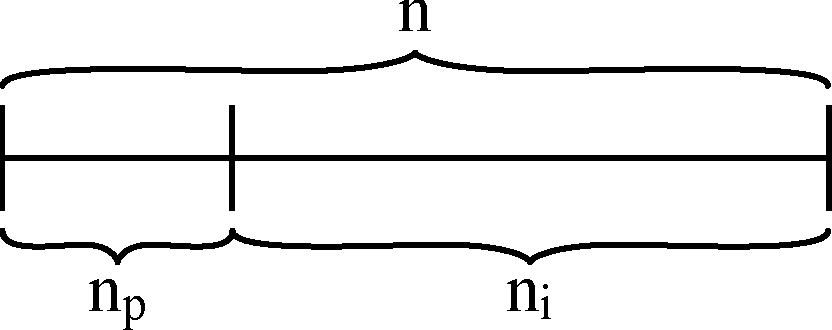
\includegraphics[scale=0.4]{HammingCode.pdf}
	\caption{Schematische Darstellung eines Hamming-Codeworts}
	\label{HammingCode}
\end{figure}

Um einen Fehler korrigieren zu können muss jede Stelle auf einen Fehler überprüft werden und es muss ein gültiges Codewort existieren. Somit müssen $n+1$ Fälle erfassen werden. Mit $n_p$ vielen Paritätsbits können $2^{n_p}$ viele Fälle codiert werden. Damit alle Fälle abgedeckt werden können muss die folgende Ungleichung erfüllt sein:
\begin{eqnarray*}
2^{n_p} &\ge& n + 1 \\
2^{n_p} &\ge& n_p + n_i + 1
\end{eqnarray*}

Beispiel: um vier Informationsbits zu sichern werden mindestens drei Paritätsbits benötigt.
\begin{eqnarray*}
2^{3} &\ge& 3 + 4 + 1 \\
8 &\ge& 8 \\
\end{eqnarray*}

Für die Einfehlerkorrektur bei Blockcodes muss jedes Informationsbit durch mindestens zwei Paritätsbits gesichert werden. Für ein Informationsbit $i$, dessen zwei Paritätsbits $p_a$ und $p_b$ und deren Paritäten $P(i, p_a)$ und $P(i, p_b)$ kann dann folgende Fallunterscheidung vorgenommen werden:
\begin{itemize}
\item
	$P(i, p_a)$ und $P(i, p_b)$ sind korrekt. Demnach sind $p_a$, $p_b$ und $i$ korrekt.
\item
	$P(i, p_a)$ und $P(i, p_b)$ sind falsch. Demnach ist $i$ falsch.
\item
	$P(i, p_a)$ ist falsch. $P(i, p_b)$ ist korrekt. Demnach ist $p_a$ falsch.
\item
	$P(i, p_a)$ ist korrekt. $P(i, p_b)$ ist falsch. Demnach ist $p_b$ falsch.
\end{itemize}
Diese Regel schließt nicht aus, dass ein Paritätsbit für mehrere Informationsbits zur Prüfung der Parität verwendet werden kann. Die Parität wird in diesem Fall nicht über zwei Bits gebildet, sondern über das jeweilige Paritätsbit inklusive der ihm zugeordneten Informationsbits. Damit eine eindeutige Fehlerlokalisierung möglich ist muss auf eine entsprechend günstige Verteilung der Informationsbits auf die Paritätsbits geachtet werden. Wenn über die Fallunterscheidung der Paritäten einem Fall genau ein Fehler zugeordnet werden kann, kann dieser Fehler entsprechend korrigiert werden.

Ein Praktisches Schema zum Finden einer optimalen Verteilung wird im folgenden Abschnitt mit Hilfe eines Beispiels erläutert.

Ein Code mit vier Informationsbits soll gesichert werden. Dazu sind drei
Paritätsbits notwendig\footnote{siehe oben}. Jedes Codewort umfasst also sieben
Stellen.
\begin{center}
\begin{tabular}{rp{3.6cm}ccccccc}
1. & die Stellen werden von $1$ 
     bis $n$ durchnummeriert.   &  1  &  2  &  3  &  4  &  5  &  6  &  7  \\
2. & die Nummerierung wird
     dual codiert.       & 00\textcolor{BrickRed}{1}
                          & 0\textcolor{RoyalBlue}{1}0 
     					   & 0\textcolor{RoyalBlue}{1}\textcolor{BrickRed}{1} 
						    & \textcolor{ForestGreen}{1}00 
						     & \textcolor{ForestGreen}{1}0\textcolor{BrickRed}{1}
						      & \textcolor{ForestGreen}{1}\textcolor{RoyalBlue}{1}0 
						       & \textcolor{ForestGreen}{1}\textcolor{RoyalBlue}{1}\textcolor{BrickRed}{1} \\
3. & das j-te Paritätsbit wird
     an der Stelle  eingetragen, 
     die im Dualcode an der j-ten Stelle eine 1 trägt. Die
     Informationsbits füllen
     der Reihe nach die 
     übrigen Stellen.           &$p_1$&$p_2$&$i_1$&$p_3$&$i_2$&$i_3$&$i_4$ \\
4. & Dem j-ten Paritätsbit
     werden diejenigen Informationsbits zugeordnet
     deren Stelle  im Dualcode an der j-ten Stelle
     eine 1 trägt. & \parbox[t]{1.5cm}{\centering $p_1$ \\ prüft \\$\{i_1,i_2,i_4\}$}
     & \parbox[t]{1.5cm}{\centering $p_2$ \\ prüft \\ $\{i_1,i_3,i_4\}$}
     & & \parbox[t]{1.5cm}{\centering $p_3$ \\ prüft \\ $\{i_2,i_3,i_4\}$} \\
5. & Die Codewörter werden erstellt.
     Im Beispiel wird das Codewort für 1010 angegeben. 
     Es wird auf gerade Parität geprüft. & 1 & 0 & 1 & 1 & 0 & 1 & 0 \\ 
     
\end{tabular}
\end{center}

Dieses Schema bietet mehrere Vorteile:
\begin{itemize}
\item
	Jedes Informationsbit wird durch mindestens zwei Paritäten geprüft.
\item
	Jedes Paritätsbit wird durch eine Parität geprüft.
\item
	Es entsteht eine optimale Zuordnung der Paritätsbits auf die Informationsbits.
\item
	Fehlercode: Wegen der Anordnung der Paritätsbits wird beim Prüfen der Paritäten die Fehlerstelle direkt über die fehlerhaften Paritäten dual codiert angezeigt. Wenn zum Beispiel die Parität über dem Paritätsbit $p_2$ fehlerhaft ist, alle anderen jedoch richtig, dann ist das fehlerhafte Bit das zweite. Wenn die Paritäten über $p_1$ und $p_2$ fehlerhaft ist, dann ist das dritte Bit fehlerhaft usw.
\end{itemize}

\chapter{Boolesche Algebra}
In diesem Artikel wird die Boolesche Algebra stark in Verbindung mit der Schaltalgebra behandelt. Deshalb werden die Zeichen 0 und 1 für die binäre Grundmenge $B = \{0,1\}$ verwendet. Weitere Unterschiede in der Notation ergeben sich bei der Besprechung der Operatoren.

\section{Operatoren}
In den folgenden Abschnitten werden die in diesem Artikel verwendeten Operatoren besprochen. Bei booleschen Operatoren kann eine endliche Wertetabelle angegeben werden, da die Grundmenge $B$ endlich ist und die Operatoren endlich viele Elemente behandeln.

\subsection{Kartesisches Produkt "`$\times$"'}
Das Kartesische Produkt wird über Mengen gebildet. Dabei werden alle Elemente der ersten Menge mit allen Elementen der zweiten Menge in einzelnen Tupeln zusammengefasst.
$$ B \times B = (0,0); (0,1); (1,0); (1,1)$$

Das $n$-fache Produkt einer Menge bezeichnet alle $n$-fachen Kombinationen aus allen Elementen der Menge.
$$ B \times B  \times B ...  \times B = B^n$$

\subsection{Negation "`NICHT"' "`NOT"' "` $\overline{a}$ "'}
Die Negation ist eine einstellige Operation, welche den Wert invertiert.
$$ f_{NOT}: B \mapsto B $$
$$ f_{NOT}(a) = \overline{a} \textnormal{ mit } a \in B$$

\begin{center}
\begin{tabular}{cc}
	$a$ & $\overline a$ \\ \hline
	0  & 1           \\
	1  & 0           \\
\end{tabular}
\end{center}

\subsection{Konjunktion "`UND"' "`AND"' "` $\cdot$ "'}
Die Konjunktion ist 1, wenn beide behandelten Werte 1 sind, ansonsten 0.
$$ f_{OR}: B \times B \mapsto B $$
$$ f_{OR}(a, b) = a \cdot b \textnormal{ mit } a, b \in B$$

\begin{center}
\begin{tabular}{ccc}
	$a$ & b & $a \cdot b$ \\ \hline
	 0  & 0 &    0    \\
	 0  & 1 &    0    \\
	 1  & 0 &    0    \\
	 1  & 1 &    1    \\
\end{tabular}
\end{center}

\subsection{Disjunktion "`ODER"' "`OR"' "` $+$ "'}
Die Disjunktion ist 1, wenn einer der behandelten Werte 1 ist, ansonsten 0.
$$ f_{OR}: B \times B \mapsto B $$
$$ f_{OR}(a, b) = a + b \textnormal{ mit } a, b \in B$$

\begin{center}
\begin{tabular}{ccc}
	$a$ & b & $a + b$ \\ \hline
	 0  & 0 &    0    \\
	 0  & 1 &    1    \\
	 1  & 0 &    1    \\
	 1  & 1 &    1    \\
\end{tabular}
\end{center}

\subsection{Äquivalenz "` $\leftrightarrow$ "'}
Die Äquivalenz ist 1, wenn beide behandelten Werte gleich sind, ansonsten 0.
$$ f_{eq}: B \times B \mapsto B $$
$$ f_{eq}(a, b) = a \leftrightarrow b \textnormal{ mit } a, b \in B$$

\begin{center}
\begin{tabular}{ccc}
	$a$ & b & $a \leftrightarrow b$ \\ \hline
	 0  & 0 &    1    \\
	 0  & 1 &    0    \\
	 1  & 0 &    0    \\
	 1  & 1 &    1    \\
\end{tabular}
\end{center}

\subsection{Antivalenz "`$XOR$"' "` $\nleftrightarrow$ "' "` $\oplus$ "'}
Die Antivalenz ist 1, wenn beide behandelten Werte ungleich sind, ansonsten 0.
$$ f_{an}: B \times B \mapsto B $$
$$ f_{an}(a, b) = a \nleftrightarrow b \textnormal{ mit } a, b \in B$$

\begin{center}
\begin{tabular}{ccc}
	$a$ & b & $a \nleftrightarrow b$ \\ \hline
	 0  & 0 &    0    \\
	 0  & 1 &    1    \\
	 1  & 0 &    1    \\
	 1  & 1 &    0    \\
\end{tabular}
\end{center}

\subsection{"`\textit{NAND}"'}
\textit{NAND} ist die Negation der Disjunktion. Mit \textit{NAND} lassen sich alle logischen Funktionen abbilden. Dies ist bei der Produktion von Hardware von Vorteil. 
$$ f_{\textit{NOR}}: B \times B \mapsto B $$
$$ f_{\textit{NOR}}(a, b) = a \textit{ NAND } b \textnormal{ mit } a, b \in B$$

\begin{center}
\begin{tabular}{ccc}
	$a$ & b & $a \textit{ NAND } b$ \\ \hline
	 0  & 0 &    1    \\
	 0  & 1 &    1    \\
	 1  & 0 &    1    \\
	 1  & 1 &    0    \\
\end{tabular}
\end{center}

\subsection{"`\textit{NOR}"'}
\textit{NOR} ist die Negation der Disjunktion. Mit \textit{NOR} lassen sich alle logischen Funktionen ebenfalls abbilden. Dies ist bei der Produktion von Hardware von Vorteil. 
$$ f_{\textit{NOR}}: B \times B \mapsto B $$
$$ f_{\textit{NOR}}(a, b) = a \textit{ NOR } b \textnormal{ mit } a, b \in B$$

\begin{center}
\begin{tabular}{ccc}
	$a$ & b & $a \textit{ NOR } b$ \\ \hline
	 0  & 0 &    1    \\
	 0  & 1 &    0    \\
	 1  & 0 &    0    \\
	 1  & 1 &    0    \\
\end{tabular}
\end{center}

\subsection{Implikation "`$\rightarrow$"'}
Die Implikation von $a$ nach $b$ ist 0, wenn $a = 0$ ist und $b = 1$, ansonsten 1. Die Implikation kann auch geschrieben werden als $(\overline{a} + b)$.
$$ f_{im}: B \times B \mapsto B $$
$$ f_{im}(a, b) = a \rightarrow b = \overline{a} + b \textnormal{ mit } a, b \in B$$

\begin{center}
\begin{tabular}{ccc}
	$a$ & b & $a \rightarrow b$ \\ \hline
	 0  & 0 &    1    \\
	 0  & 1 &    1    \\
	 1  & 0 &    0    \\
	 1  & 1 &    1    \\
\end{tabular}
\end{center}

\section{Grundlegende Gesetze}
Es gelten folgende grundlegende Gesetze in der booleschen Algebra:

\subsection*{Kommutativ-Gesetze}
\begin{align*}
	a \cdot b & = b \cdot a \\
	a + b & = b + a \\
\end{align*}

\subsection*{Assoziativ-Gesetze}
\begin{align*}
	(a \cdot b) \cdot c & = a \cdot (b \cdot c) \\
	(a + b) + c & = a + (b + c) \\
\end{align*}

\subsection*{Distributiv-Gesetze}
\begin{align*}
	a \cdot (b + c) & = (a \cdot b) + (a \cdot c) \\
	a + (b \cdot c) & = (a + b) \cdot (a + c) \\
\end{align*}

\subsection*{Neutrale Elemente}
\begin{align*}
	a \cdot 1 & = a \\
		a + 0 & = a \\
	a \cdot a & = a \\
		a + a & = a \\
\end{align*}

\subsection*{Komplemente}
\begin{align*}
	a \cdot \overline{a} & = 0 \\
		a + \overline{a} & = 1 \\
\end{align*}

\subsection*{Negation der Negation}
\begin{align*}
	\overline{\overline{a}} & = a \\
\end{align*}

\subsection*{Gesetze nach De Morgan und Shannon}
\begin{align*}
	\overline{a \cdot b} & = \overline a + \overline b \\
	\overline{a + b} & = \overline a \cdot \overline b \\
	\overline{a \leftrightarrow b} 
		& = \overline a \nleftrightarrow \overline b \\
	\overline{a \nleftrightarrow b} 
		& = \overline a \leftrightarrow \overline b \\
\end{align*}

\subsection*{Absorptionsgesetze}
\begin{align*}
	a + (a \cdot b) = a \\
	a \cdot (a + b) = a \\
\end{align*}

In diesem Artikel werden folgende Bindungsstärken festgelegt:
\begin{enumerate}
\item
	Negation bindet stärker als Konjunktion
\item
	Konjunktion bindet stärker als Disjunktion
\end{enumerate}

Das Konjunktionsszeichen "` $\cdot$ "' zwischen Operanden wird zur Vereinfachung der Schreibweise weggelassen.

\section{Entwurf von Schaltnetzen}
Logische Funktionenen werden hardware-technisch in Logikgattern produziert. Wegen der hohen Flexibilität der Booleschen Algebra können verschiedene Gatteranordnungen gleiche Funktionen repräsentieren. Also ist Ziel des Entwurfs eine aufwandsgünstigste Lösung zu finden. Mit der heutigen Halbleitertechnologie werden hochintegrierte Schaltkreise gefertigt. Um den Testaufwand zu vereinfachen werden möglichst regelmäßige Strukturen bevorzugt.

Jede logische Funktionsvorschrift lässt sich als Funktionstabelle\footnote{Funktionstabelle: auch genannt Schaltbelegungstabelle; Krzl. SBT} oder Term\footnote{Term wird hier synonym für mathematischer Ausdruck verwendet} darstellen. Die Funktionsterme dienen als Vorlage für den Gatterbau. Nach den Regeln der Boolschen Algebra können Funktionsterme umgeformt und so in eine optimale Form gebracht werden. Zur Entwicklung des Gatterentwurfs werden in der Praxis \textsc{Silicon}-Compiler Programme eingesetzt.

\subsection{Definition der Booleschen Normalformen}
Ein Boolescher Funktionsterm kann aus mehreren Eingabe-Variablen oder deren Negation und deren logischen Verknüpfungen bestehen.

\textbf{Die Konjunktive Form (KF)} einer logischen Funktion ist die Konjunktion von Disjunktionen. Beispiel:
$$ f_{\textit{KF}}(a,b,c,d) = (a + c) \cdot (\overline{c} + d)
	\cdot (\overline{a} + c + d) $$

\textbf{Die Disjunktive Form (DF)} einer logischen Funktion ist die Disjunktion von Konjunktionen. Beispiel:
$$ f_{\textit{DF}}(a,b,c,d) = (a \cdot c) + (\overline{a} \cdot d)
	+ (\overline{a} \cdot b \cdot d) $$

\textbf{Die kanonische Normalform} eines Funktionsterms ist die Form in der alle Variablen der Funktion, entweder als solche oder negiert, in einer Disjunktiven Form oder Konjunktiven Form verknüpft sind. Die jeweilige Form wird \textsl{Disjunktive kanonische Normalform (DNF)} bzw. \textsl{Konjunktive kanonische Normalform (KNF)} genannt. Beispiele:
$$ f_{\textit{KNF}}(a,b,c,d) = 
	\underbrace{(a + \overline{b} + c + d)}_{Maxterm / Faktor}
	\cdot (a + b +\overline{c} + d) 
	\cdot (\overline{a} + \overline{b} + c + d) $$
$$ f_{\textit{DNF}}(a,b,c,d) = 
	\underbrace{(a \cdot b \cdot c \cdot d)}_{Minterm / Summand}
	+ (\overline{a} \cdot \overline{b} \cdot \overline{c} \cdot d)
	+ (\overline{a} \cdot b \cdot c \cdot d) $$
Die Faktoren der Konjunktiven kanonischen Normalform werden Maxterme genannt. Die Summanden der Disjunktiven kanonischen Normalform heißen Minterme.

Jeder logische Term lässt sich in der Konjunktiven Form oder der Disjunktiven Form darstellen. Durch Erweiterung kann jeder Term außerdem in die Disjunktive oder Konfjunktive Normalform gebracht werden. Die Disjunktive Form wird durch "`Ausmultiplizieren"' und die Konjunktive Form durch "`Ausaddieren"' erstellt.

Eine Disjunktive Formen kann in die Disjunktive Normalform umgeformt werden indem den Summanden das für Konjunktionen neutrale Element $1 = (x + \overline{x})$ je nach fehlender Variable hinzugefügt wird. Anschließend muss wiederum ausmultipliziert werden. Entsprechend kann die Konjunktive Normalform erschlossen werden indem den Faktoren das für Disjunktionen neutrale Element $0 = (x \cdot \overline{x})$ je nach fehlender Variable hinzugefügt wird. Danach wird wieder ausaddiert.

Beispiel: Der Funktionsterm $f = a(b + c) + c(a + \overline{b}c)$ soll in Konjunktive bzw. Disjunktive Form umgeformt werden. Anschließend werden die erhaltenen Formen in die Normalform überführt.

Umformung in Disjunktive Form durch "`Ausmultiplizieren"' (siehe Abbildung \ref{Ausmultiplizieren}):

\begin{figure}[htbp] % positioning htbp: h = here; t = top; b bottom; p own page
	\centering
	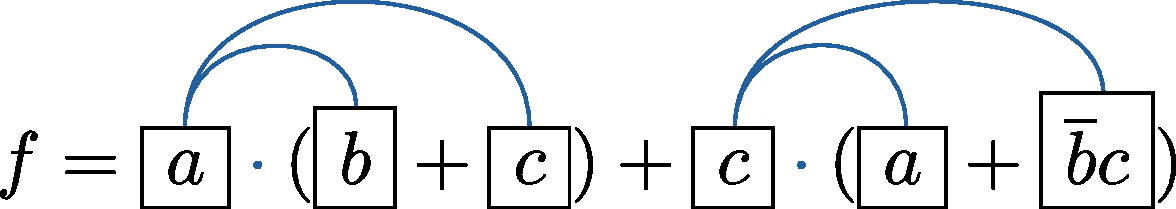
\includegraphics[scale=0.4]{Ausmultiplizieren.pdf}
	\caption{Ausmultiplizieren}
	\label{Ausmultiplizieren}
\end{figure}
\begin{align*}
				  f &= a(b + c) + c(a + \overline{b}c) \\
					&= ab + ac + ca + c\overline{b}c   \\
	f_{\textit{DF}} &= ab + ac + \overline{b}c    \\
\end{align*}

Umformung in Konjunktive Form durch "`Ausaddieren"' (siehe Abbildung \ref{Ausaddieren}):

\begin{figure}[htbp] % positioning htbp: h = here; t = top; b bottom; p own page
	\centering
	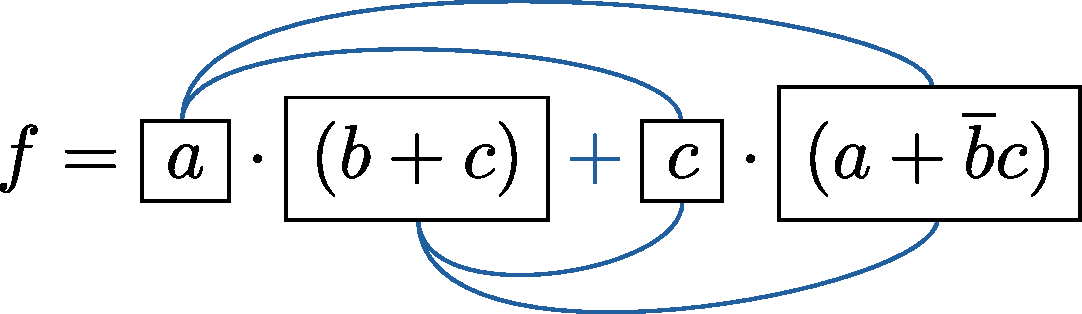
\includegraphics[scale=0.4]{Ausaddieren.pdf}
	\caption{Ausaddieren}
	\label{Ausaddieren}
\end{figure}

\begin{align*}
				  f &= a(b + c) + c(a + \overline{b}c)                \\
					&= (a + c) (a + (a + \overline{b}c))
						((b + c) + c) ((b + c) + (a + \overline{b}c)) \\
	                &= (a + c) (a + \overline{b}c)
					   (b + c) (b + a 
					   + \underbrace{c + \overline{b}c}_{Absorption}) \\
	                &= (a + c) (a + \overline{b}c) (b + c) (a + b + c) \\
	                &= (a + c) (a + \overline{b}) (a + c) 
	                   (b + c) (a + b + c) \\
	f_{\textit{KF}} &= (a + c) (a + \overline{b}) (b + c) \\
\end{align*}

Herleitung der Disjunktiven Normalform durch Hinzufügen neutraler Elemente der Form $(x + \overline{x})$:
\begin{align*}
	f_{\textit{DF}} &= ab + ac + \overline{b}c    \\
	                &= ab(c + \overline{c})
	                 + ac(b + \overline{b})
	                 + \overline{b}c(a + \overline{a})    \\
	                &= abc + ab\overline{c}
	                 + acb + ac\overline{b}
	                 + \overline{b}ca + \overline{b}c\overline{a}    \\
	f_{\textit{DNF}} &= abc + ab\overline{c} + a\overline{b}c
	                  + \overline{a}\overline{b}c    \\
\end{align*}

Herleitung der Konjunktiven Normalform durch Hinzufügen neutraler Elemente der Form $(x \cdot \overline{x})$:

\begin{align*}
	f_{\textit{DF}} &= (a + c) (a + \overline{b}) (b + c) \\
					&= (a + c + (b \cdot \overline{b})) 
						(a + \overline{b} + (c \cdot \overline{c})) 
						(b + c + (a \cdot \overline{a})) \\
					&= ((a + c + b) \cdot (a + c + \overline{b})) 
						((a + \overline{b} + c) \cdot 
						(a + \overline{b} + \overline{c}))
						((b + c + a) \cdot (b + c + \overline{a})) \\
					&= (a + b + c) (a + \overline{b} + c)
						(a + \overline{b} + \overline{c})
						(\overline{a} + b + c) \\
\end{align*}

Die Minterme beziehungsweise Maxterme einer logischen Funktion sind eindeutig bestimmt. Demnach besitzt jede logische Funktion genau eine Konjunktive und eine Disjunktive kanonische Normalform. Sie bilden den Ausgangspunkt allgemeingültiger Reduktionsmethoden.

\subsection{Schaltbelegungstabelle}
Logische Funktionen können auch mittels einer Schaltbelegungstabelle spezifiziert werden. Die Min- und Maxterme können aus dieser Tabelle direkt ausgelesen und damit die kanonischen Normalformen erstellt werden. Zur Erstellung der Schaltbelegungstabelle werden für eine $n$-stellige Funktion alle $2^n$ Kombinationen der Eingangsvariablen aufgeschrieben und das jeweilige Ergebnis dazu notiert. Damit ist für alle Eingangswerte der Funktion das Ergebnis der Funktion definiert. Beispiel:

%\begin{tabular}{lc*{8}{c}}
%BitNr.        & $i$              &        0      &             1            &              2              &                  3                  &                 4           &        5         &                 6                   &                       7                        \\ \hline
%Variable      & $a$              &        0      &             1            &              0              &                  1                  &                 0           &        1         &                 0                   &                       1                        \\
%              & $b$              &        0      &             0            &              1              &                  1                  &                 0           &        0         &                 1                   &                       1                        \\
%              & $c$              &        0      &             0            &              0              &                  0                  &                 1           &        1         &                 1                   &                       1                        \\ \hline
%Funktionswert & $y$              &        0      &             0            &              1              &                  0                  &                 1           &        1         &                 0                   &                       0                        \\
%\hline\noalign{\smallskip}                                                                                                                                                                                                                                                              
%Minterme DNF  & $f_\textit{DNF}$ &               &                          & $\overline{a}b\overline{c}$ &                                     & $\overline{a}\overline{b}c$ & $a\overline{b}c$ &                                     &                                                \\
%\hline\noalign{\smallskip}
%Maxterme KNF  & $f_\textit{KNF}$ & $(a + b + c)$ & $(\overline{a} + b + c)$ &                             & $(\overline{a} + \overline{b} + c)$ &                             &                  & $(a + \overline{b} + \overline{c})$ & $(\overline{a} + \overline{b} + \overline{c})$ \\
%\end{tabular}

\begin{table}
\caption{Schaltbelegungstabelle für $f(a, b, c)$}
\label{SBT_bsp}
\resizebox{1\textwidth}{!} {
\begin{tabular}{c*{8}{c}}
$i$              &        0      &             1            &              2              &                  3                  &                 4           &        5         &                 6                   &                       7                        \\ \hline
$a$              &        0      &             0            &              0              &                  0                  &                 1           &        1         &                 1                   &                       1                        \\ 
$b$              &        0      &             0            &              1              &                  1                  &                 0           &        0         &                 1                   &                       1                        \\
$c$              &        0      &             1            &              0              &                  1                  &                 0           &        1         &                 0                   &                       1                        \\ \hline
$y$              &        0      &             0            &              1              &                  0                  &                 1           &        1         &                 0                   &                       0                        \\
\hline\noalign{\smallskip}                                                                                                                                                                                                                                                              
$m_i$            &               &                          & $\overline{a}b\overline{c}$ &                                     & $a\overline{b}\overline{c}$ & $a\overline{b}c$ &                                     &                                                \\
\hline\noalign{\smallskip}
$M_i$            & $(a + b + c)$ & $(a + b + \overline{c})$ &                             & $(a + \overline{b} + \overline{c})$ &                             &                  & $(\overline{a} + \overline{b} + c)$ & $(\overline{a} + \overline{b} + \overline{c})$ \\
\end{tabular}
}
\end{table}

Die Schaltbelegungstabelle gibt die Belegungen der Variablen an, bei denen der Funktionswert 1 ist. Da eine Disjunktion genau dann 1 ist, wenn eines ihrer Summanden 1 ist, lassen sich die Minterme aus der Schaltbelegungstabelle ablesen. Ein Minterm ergibt sich aus jeder Spalte, in der der Funktionswert 1 ist. Ist die Belegung der Variable in dieser Spalte 1, dann muss im Minterm die Variable als solche angegeben werden. Ist die Belegung der Variable 0, dann muss im Minterm die negierte Variable angegeben werden (vgl. Tabelle \ref{SBT_bsp} Spalten $i \in \{2, 4, 5\}$). Im angegebenen Beispiel ist die Disjunktive kanonische Normalform der Funktion $f(a,b,c)$ also:
\begin{align*}
 \sum_{i \in \{2, 4, 5\}} m_i &= \sum m(2, 4, 5) \\
m_2 + m_4 + m_5 &= \overline{a}b\overline{c} + a\overline{b}\overline{c} + a\overline{b}c
\end{align*}

Für die Herleitung der Maxterme betrachten wir zuerst die negierte Funktion. Die Minterme der negierten Funktion befinden sich an genau den Stellen, an der die Funktion ihre Maxterme hat. Über Negation der negierten Funktion wird wieder die ursprüngliche Funktion erzeugt. Die negierten Minterme der negierten Funktion sind nach De Morgan also die Maxterme der ursprünglichen Funktion.

Mit den Maxtermen kann analog folgendermaßen verfahren werden: Die Schaltbelegungstabelle gibt die Belegungen der Variablen an, bei denen der Funktionswert 0 ist. Ein Maxterm ergibt sich aus jeder Spalte, in der der Funktionswert 0 ist. Ist die Belegung der Variable in dieser Spalte 1, dann muss im Maxterm die negierte Variable angegeben werden. Ist die Belegung der Variable 0, dann muss im Maxterm die Variable als solche angegeben werden (vgl. Tabelle \ref{SBT_bsp} Spalten $i \in \{0, 1, 3, 6, 7\}$)\footnote{also salopp genau anders herum als vorher}. Im angegebenen Beispiel ist die Konjunktive kanonische Normalform der Funktion $f(a,b,c)$ also:
\begin{align*}
 \prod_{i \in \{0, 1, 3, 6, 7\}} M_i &= \prod M(0, 1, 3, 6, 7) \\
M_0 \cdot M_1 \cdot M_3 \cdot M_6 \cdot M_7 &= (a + b + c)(a + b + \overline{c})(a + \overline{b} + \overline{c})(\overline{a} + \overline{b} + c)(\overline{a} + \overline{b} + \overline{c})
\end{align*}

\subsection{Redundante Funktionen}
In manchen Fällen kommen bestimmte Kombinationen der Belegung der Eingabevariablen nie vor. Folglich müssen Funktionswerte für diese Kombinationen nicht zwingend definiert werden. Der Funktionswert in solchen Fällen ist also beliebig. In der Schalttabelle werden nicht definierte Funktionswerte mit "` * "' gekennzeichnet. Bei der Optimierung können nicht zuerst nicht definierte Funktionswerte frei gewählt werden und können gegebenenfalls für so für eine Optimierung sorgen, die anders nicht möglich gewesen wäre.

\subsection{Reduktion von Schaltfunktionenen (Minimierung)}
Die Komplexität von Schaltfunktionen wird reduziert um folgende Vorteile zu nutzen:
\begin{itemize}
	\item
		Vereinfachung der logischen Funktionsterme
	\item
		Verringerung der Schaltnetzkosten (Gatteranzahl, chip-/board-Fläche, Energie usw.)
	\item
		Zuverlässigkeit
\end{itemize}
"`Regelmäßige"' Schaltfunktionen haben demgegenüber folgende Vorteile:
\begin{itemize}
  \item regelmäßige Lösungsstrukturen
  \item Geringerer Wartungs-, Pflege und Entwurfsaufwand
  \item Es können \textsc{vls(i)}-Schaltkeise (\textsc{prom}, \textsc{pal}, \textsc{gal}, \textsc{fpga} usw.)
\end{itemize}
Zur Reduktion können unterschiedliche Verfahren verwendet werden:
\begin{itemize}
  \item Algebraische Reduktion
  \item Grafische Reduktion
  \item Algorithmische Reduktion
\end{itemize}

Logische Terme können durch Hinzufügen neutraler Elemente erweitert werden. $0$ ist das neutrale Element der Disjunktion. $0$ kann auch anders geschrieben werden als: 
$$ 
	0 = x \cdot \overline{x} \hspace{5mm} \textnormal{mit } x \textnormal{ als logischer Term}
$$
Also kann jeder logischer Term disjunktiv mit $x \cdot \overline{x}$ verknüpft werden ohne, dass sich der Wert des Terms ändert.
$$ 
	a = a + (x \cdot \overline{x}) \hspace{5mm} \textnormal{mit } x, a \textnormal{ als logische Terme}
$$

Analog gilt für das neutralen Element $1$ der Konjunktion:
$$
	1 = x + \overline{x} \hspace{5mm} \textnormal{mit } x \textnormal{ als logischer Term}
$$
und jeder Term kann konjunktiv mit $x \cdot \overline{x}$ verknüpft werden ohne, dass sich der Wert des Terms ändert.
$$ 
	a = a \cdot (x + \overline{x}) \hspace{5mm} \textnormal{mit } x, a \textnormal{ als logische Terme}
$$

Um einen Funktioinsterm zu minimieren müssen diese neutralen Elemente aus dem Funktionsterm eliminiert werden. Bei der Disjunktiven Kanonischen Normalform lässt sich die Form ausnutzen indem Summanden gesucht werden, deren Faktoren ähnlich sind. Ähnlich in diesem Fall bedeutet, dass die Faktoren der beiden zu betrachtenden Summanden gleich sind mit Ausnahme eines Faktors, welcher im einen Summand als solcher vorkommt und im anderen negiert. Dann lassen sich die gleichen Faktoren der Summanden ausklammern und aus den beiden übrigen Faktoren ergibt sich das Neutrale Element zur Disjunktion und entfallen daher. Beispiel:
\begin{align*}
	f_{\textit{DNF}} &= \overline{a}\overline{b}c + \overline{a}b\overline{c} 
		+ \underbrace{a\overline{b}\overline{c} + ab\overline{c}}_{\textnormal{ähnlich}} \\
	&= \overline{a}\overline{b}c + \overline{a}b\overline{c} 
		+ a(\overline{b}\overline{c} + b\overline{c}) \\
	&= \overline{a}\overline{b}c + \overline{a}b\overline{c} 
		+ a\overline{c}(\overline{b} + b) \\
	&= \overline{a}\overline{b}c + \overline{a}b\overline{c} 
		+ a\overline{c} \cdot 1 \\
	f_{\textit{DF}} &= \overline{a}\overline{b}c + \overline{a}b\overline{c}
		+ a\overline{c} \\
\end{align*}

Die Form der Konjunktiven Kanonischen Normalform lässt sich analog über das neutrale Element der Konjunktion zur Minimierung nutzen. Es werden Faktoren gesucht, deren Summanden ähnlich sind. Beispiel:
% TODO Ausführlichere Beschreibung 
\begin{align*}
	f_{\textit{KNF}} &= (\overline{a} + \overline{b} + c) \cdot (\overline{a} + b + \overline{c}) 
		\cdot \underbrace{(a + \overline{b} + \overline{c}) \cdot (a + b + \overline{c})}_{\textnormal{ähnlich}} \\
	&= (\overline{a} + \overline{b} + c) \cdot (\overline{a} + b + \overline{c}) 
		\cdot (a + (\overline{b} + \overline{c}) \cdot (b + \overline{c})) \\
	&= (\overline{a} + \overline{b} + c) \cdot (\overline{a} + b + \overline{c}) 
		\cdot (a + \overline{c} + (\overline{b} \cdot b)) \\
	&= (\overline{a} + \overline{b} + c) \cdot (\overline{a} + b + \overline{c}) 
		\cdot (a + \overline{c} + 0) \\
	f_{\textit{KF}} &= (\overline{a} + \overline{b} + c) \cdot (\overline{a} + b + \overline{c}) 
		\cdot (a + \overline{c}) \\
\end{align*}

Um die Suche nach den neutralen Elementen für uns Menschen zu erleichtern wurde eine Grafische Methode zur Funktionsminimierung entwickelt. Kanonische Normalformen können mit Karnaugh-Veitch-Diagrammen\footnote{Karnaugh-Veitch-Diagramm kurz KV-Diagramm} grafisch dargestellt und reduziert werden. Die mathematische Grundlage dafür bilden die neutralen Elemente und deren Umformung, wie zuvor beschrieben.

%TODO Ergänzen: Eine 1 darf in mehreren Gruppen enthalten sein, da 1 für Term der Fkt steht und Aussage durch hinzufügen identischer terme nicht verändert wird
%TODO Gruppen anhand algebraischer Zusammenhänge erklären. 2*2er Grp -> 2Grp -> zusammengefasster Term

Je nach Anzahl der Eingangsvariablen eines Funktionsterms wird das KV-Diagramm erweitert. Abbildung \ref{KVdiag_Entw} zeigt den Aufbau der KV-Diagramme für eins, zwei, drei und vier Variablen. Wie in der Abbildung zu sehen, sind die Bereiche des Diagramms passend für alle Kombinationen der Variablen aufgeteilt.

\begin{figure}[htbp] % positioning htbp: h = here; t = top; b bottom; p own page
	\centering
	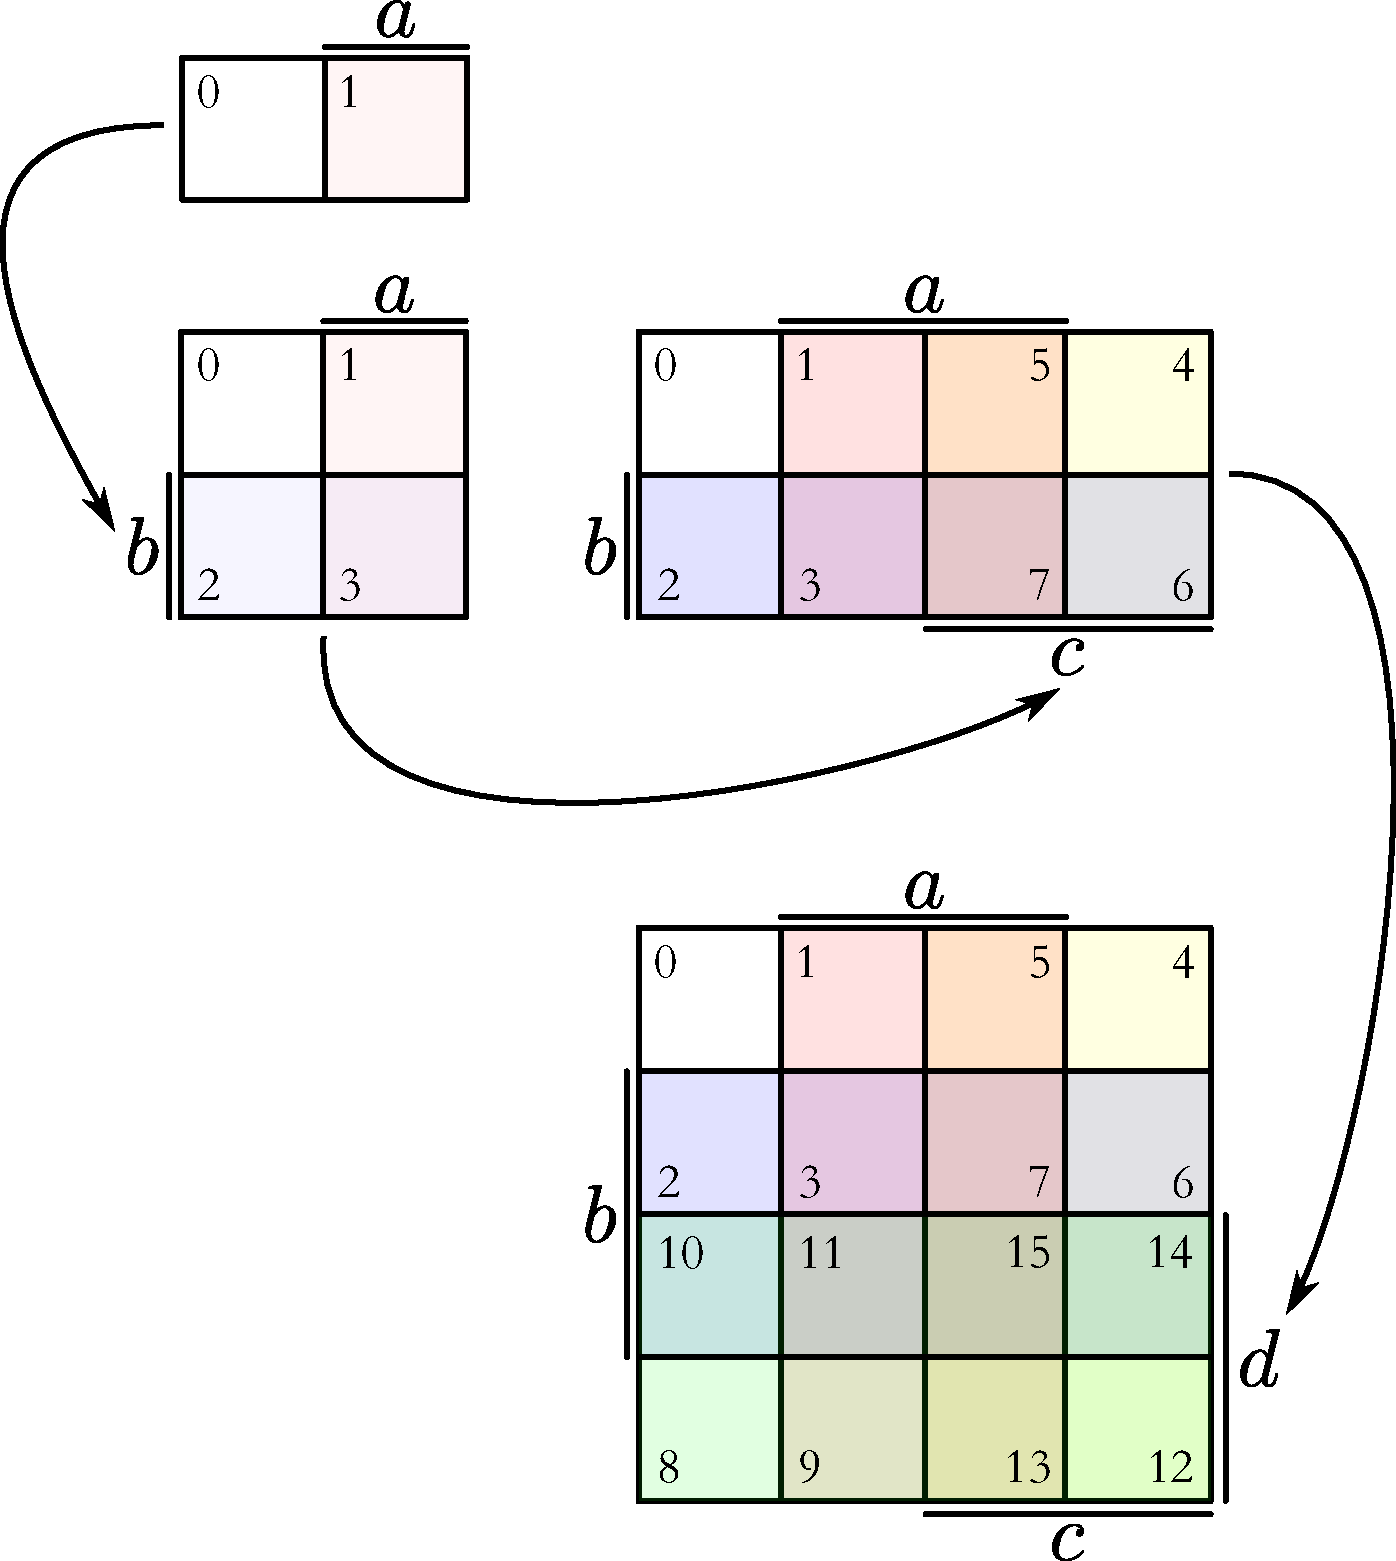
\includegraphics[width=0.8\textwidth]{KVdiagramm_Entwicklung.pdf}
	\caption{Entwicklung der KV-Diagramme für eins bis vier Variablen}
	\label{KVdiag_Entw}
\end{figure}

Mit dem Buchstaben der Variable und einem "` | "' wird definiert in welchem Bereich die Variable den Wert $1$ hat. In allen anderen Bereichen hat die Variable den Wert $0$. So können die Funktionswerte aus der Schaltbelegungstabelle direkt in ein Diagramm übernommen werden. Das Diagramm kann also als weitere Darstellungsform einer logischen Funktion benutzt werden.

Damit die Übertragung aus der Schaltbelegungstabelle möglichst einfach wird, sollte die Belegung wie im folgenden Beispiel dargestellt gewählt werden. Die Kombinationen werden durchnummeriert anhand der Dualzahlendarstellung der jeweiligen Kombination. Die Variable mit der lexikografisch niedrigsten Ziffer bekommt die niedrigste Stellenwertigkeit (vgl. Tabelle \ref{SBT_bsp}). So können die Funktionswerte der nummerierten Kombinationen nach den Zahlen in Abbildung \ref{KVdiag_Entw} korrekt übertragen werden ohne viele Überlegungen machen zu müssen. 

\begin{table}
\centering
	\begin{tabular}[htbp]{c*{16}{c}}
		$i$ & 0 & 1 & 2 & 3 & 4 & 5 & 6 & 7 & 8 & 9 &10 &11 &12 &13 &14 &15 \\ \hline
		$a$ & 0 & 1 & 0 & 1 & 0 & 1 & 0 & 1 & 0 & 1 & 0 & 1 & 0 & 1 & 0 & 1 \\ 
		$b$ & 0 & 0 & 1 & 1 & 0 & 0 & 1 & 1 & 0 & 0 & 1 & 1 & 0 & 0 & 1 & 1 \\
		$c$ & 0 & 0 & 0 & 0 & 1 & 1 & 1 & 1 & 0 & 0 & 0 & 0 & 1 & 1 & 1 & 1 \\
		$d$ & 0 & 0 & 0 & 0 & 0 & 0 & 0 & 0 & 1 & 1 & 1 & 1 & 1 & 1 & 1 & 1 \\ \hline
		$f$ & 1 & 0 & 0 & 0 & 1 & 0 & 1 & 1 & 1 & 0 & 0 & 0 & 1 & 0 & 1 & 1 \\
	\end{tabular}
\caption{SBT zur Referenz für eine günstige Anordnung der 16 Kombinationen von $a, b, c, d$}
\label{SBT_bsp}
\end{table}

Abbildung \ref{KVdiag_bsp_ausgefuellt} zeigt das Diagramm zu Tabelle \ref{SBT_bsp}.
\begin{figure}[htbp] % positioning htbp: h = here; t = top; b bottom; p own page
	\centering
	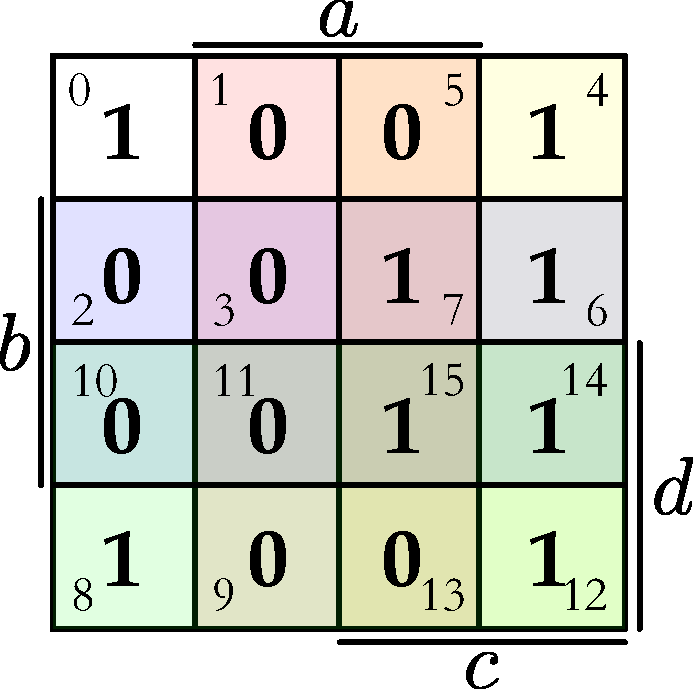
\includegraphics[scale = 0.5]{KVdiagramm_KVdiagramm_abcd_ausgefuellt.pdf}
	\caption{Ausgefülltes Diagramm zu Tabelle \ref{SBT_bsp}}
	\label{KVdiag_bsp_ausgefuellt}
\end{figure}

Felder, die sich durch Negation einer einzigen Variablen unterscheiden, werden benachbart genannt. Benachbarte Felder sind teilweise sofort im planaren Raum der Diagramme als Felder in direkter Nachbarschaft ersichtlich. Beim Diagramm für drei Variablen kommt es zusätzlich zu einer Ringbildung der Seiten. Damit sind im KV$_3$-Diagramm die Felder 0 mit 4 und 2 mit 6 benachbart. 

Im KV$_4$-Diagramm ist der linke Rand mit dem rechten und der obere Rand mit dem unteren miteinander benachbart. Im KV$_4$-Diagramm sind also, neben den offensichtlichen, die Felder 0 mit 4, 2 mit 6, 10 mit 14, 8 mit 12, 0 mit 8, 1 mit 9, 5 mit 13 und 4 mit 12 benachbart. Die Abbildung \ref{KVdiag_nachbarschaften} veranschaulicht die weniger offensichtlichen Nachbarschaften.

\begin{figure}[htbp] % positioning htbp: h = here; t = top; b bottom; p own page
	\centering
	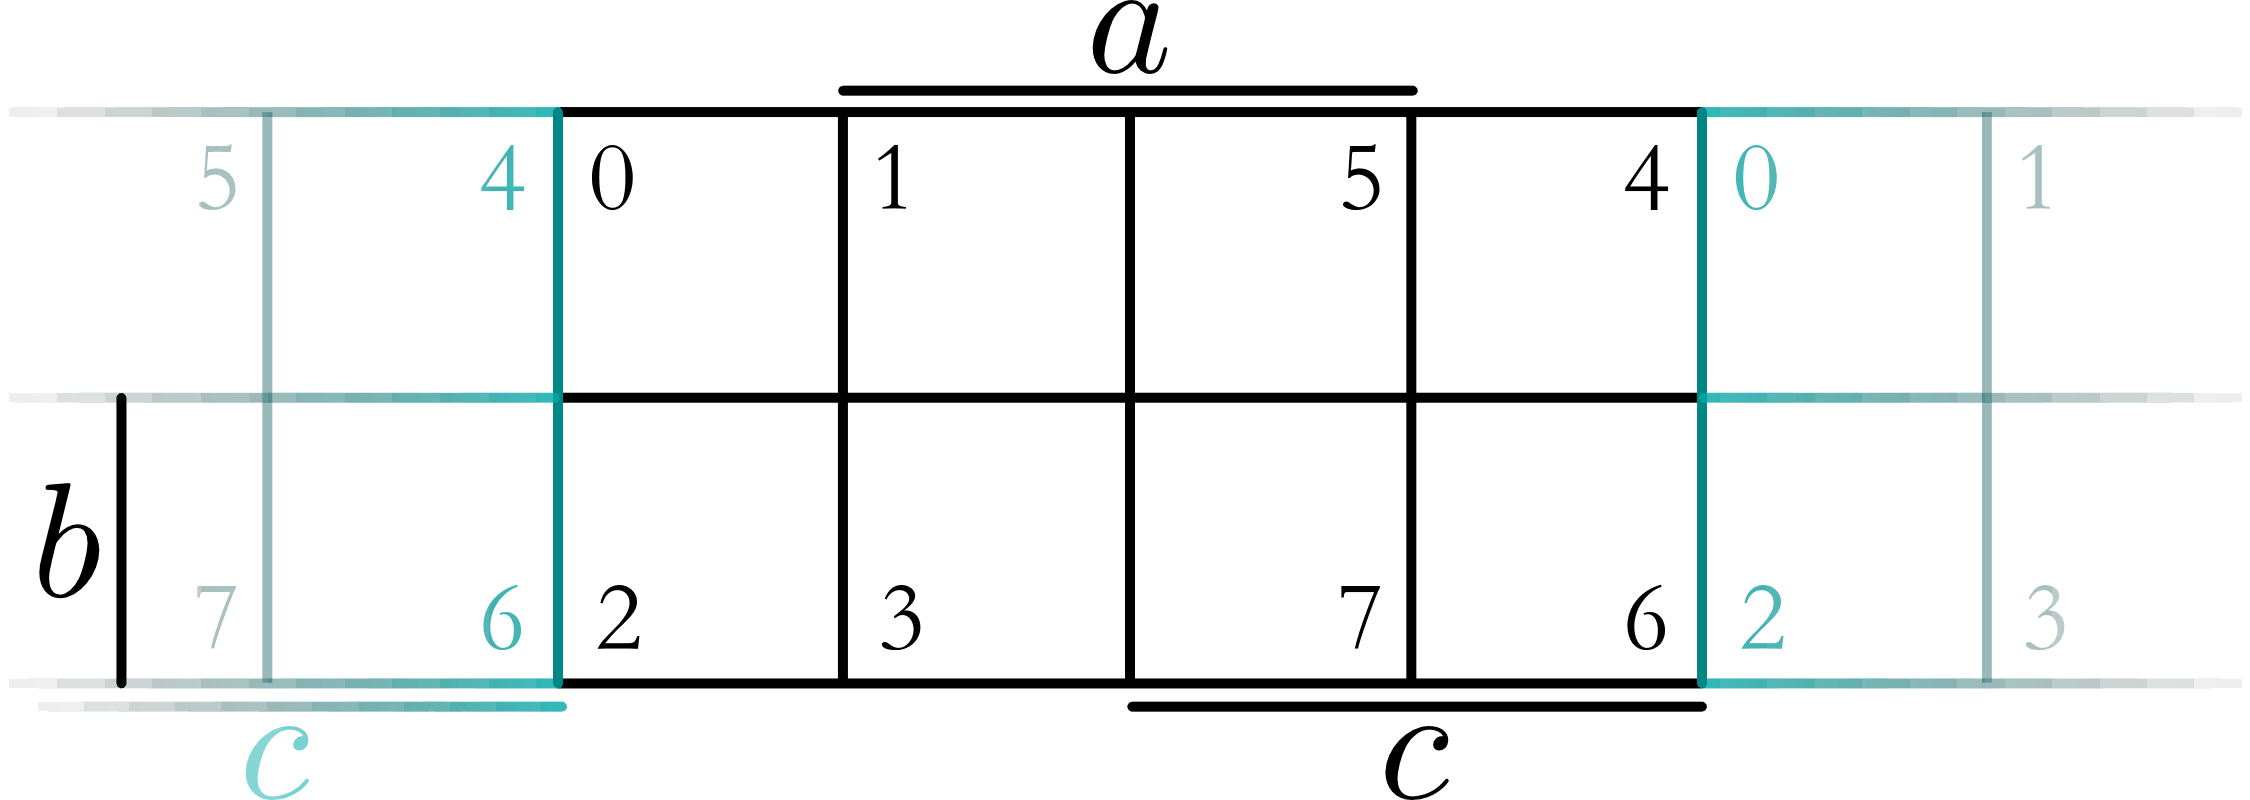
\includegraphics[scale = 0.5]{KV3diagramm_Nachbarschaften.png}
	
	\vspace{.6cm}
	
	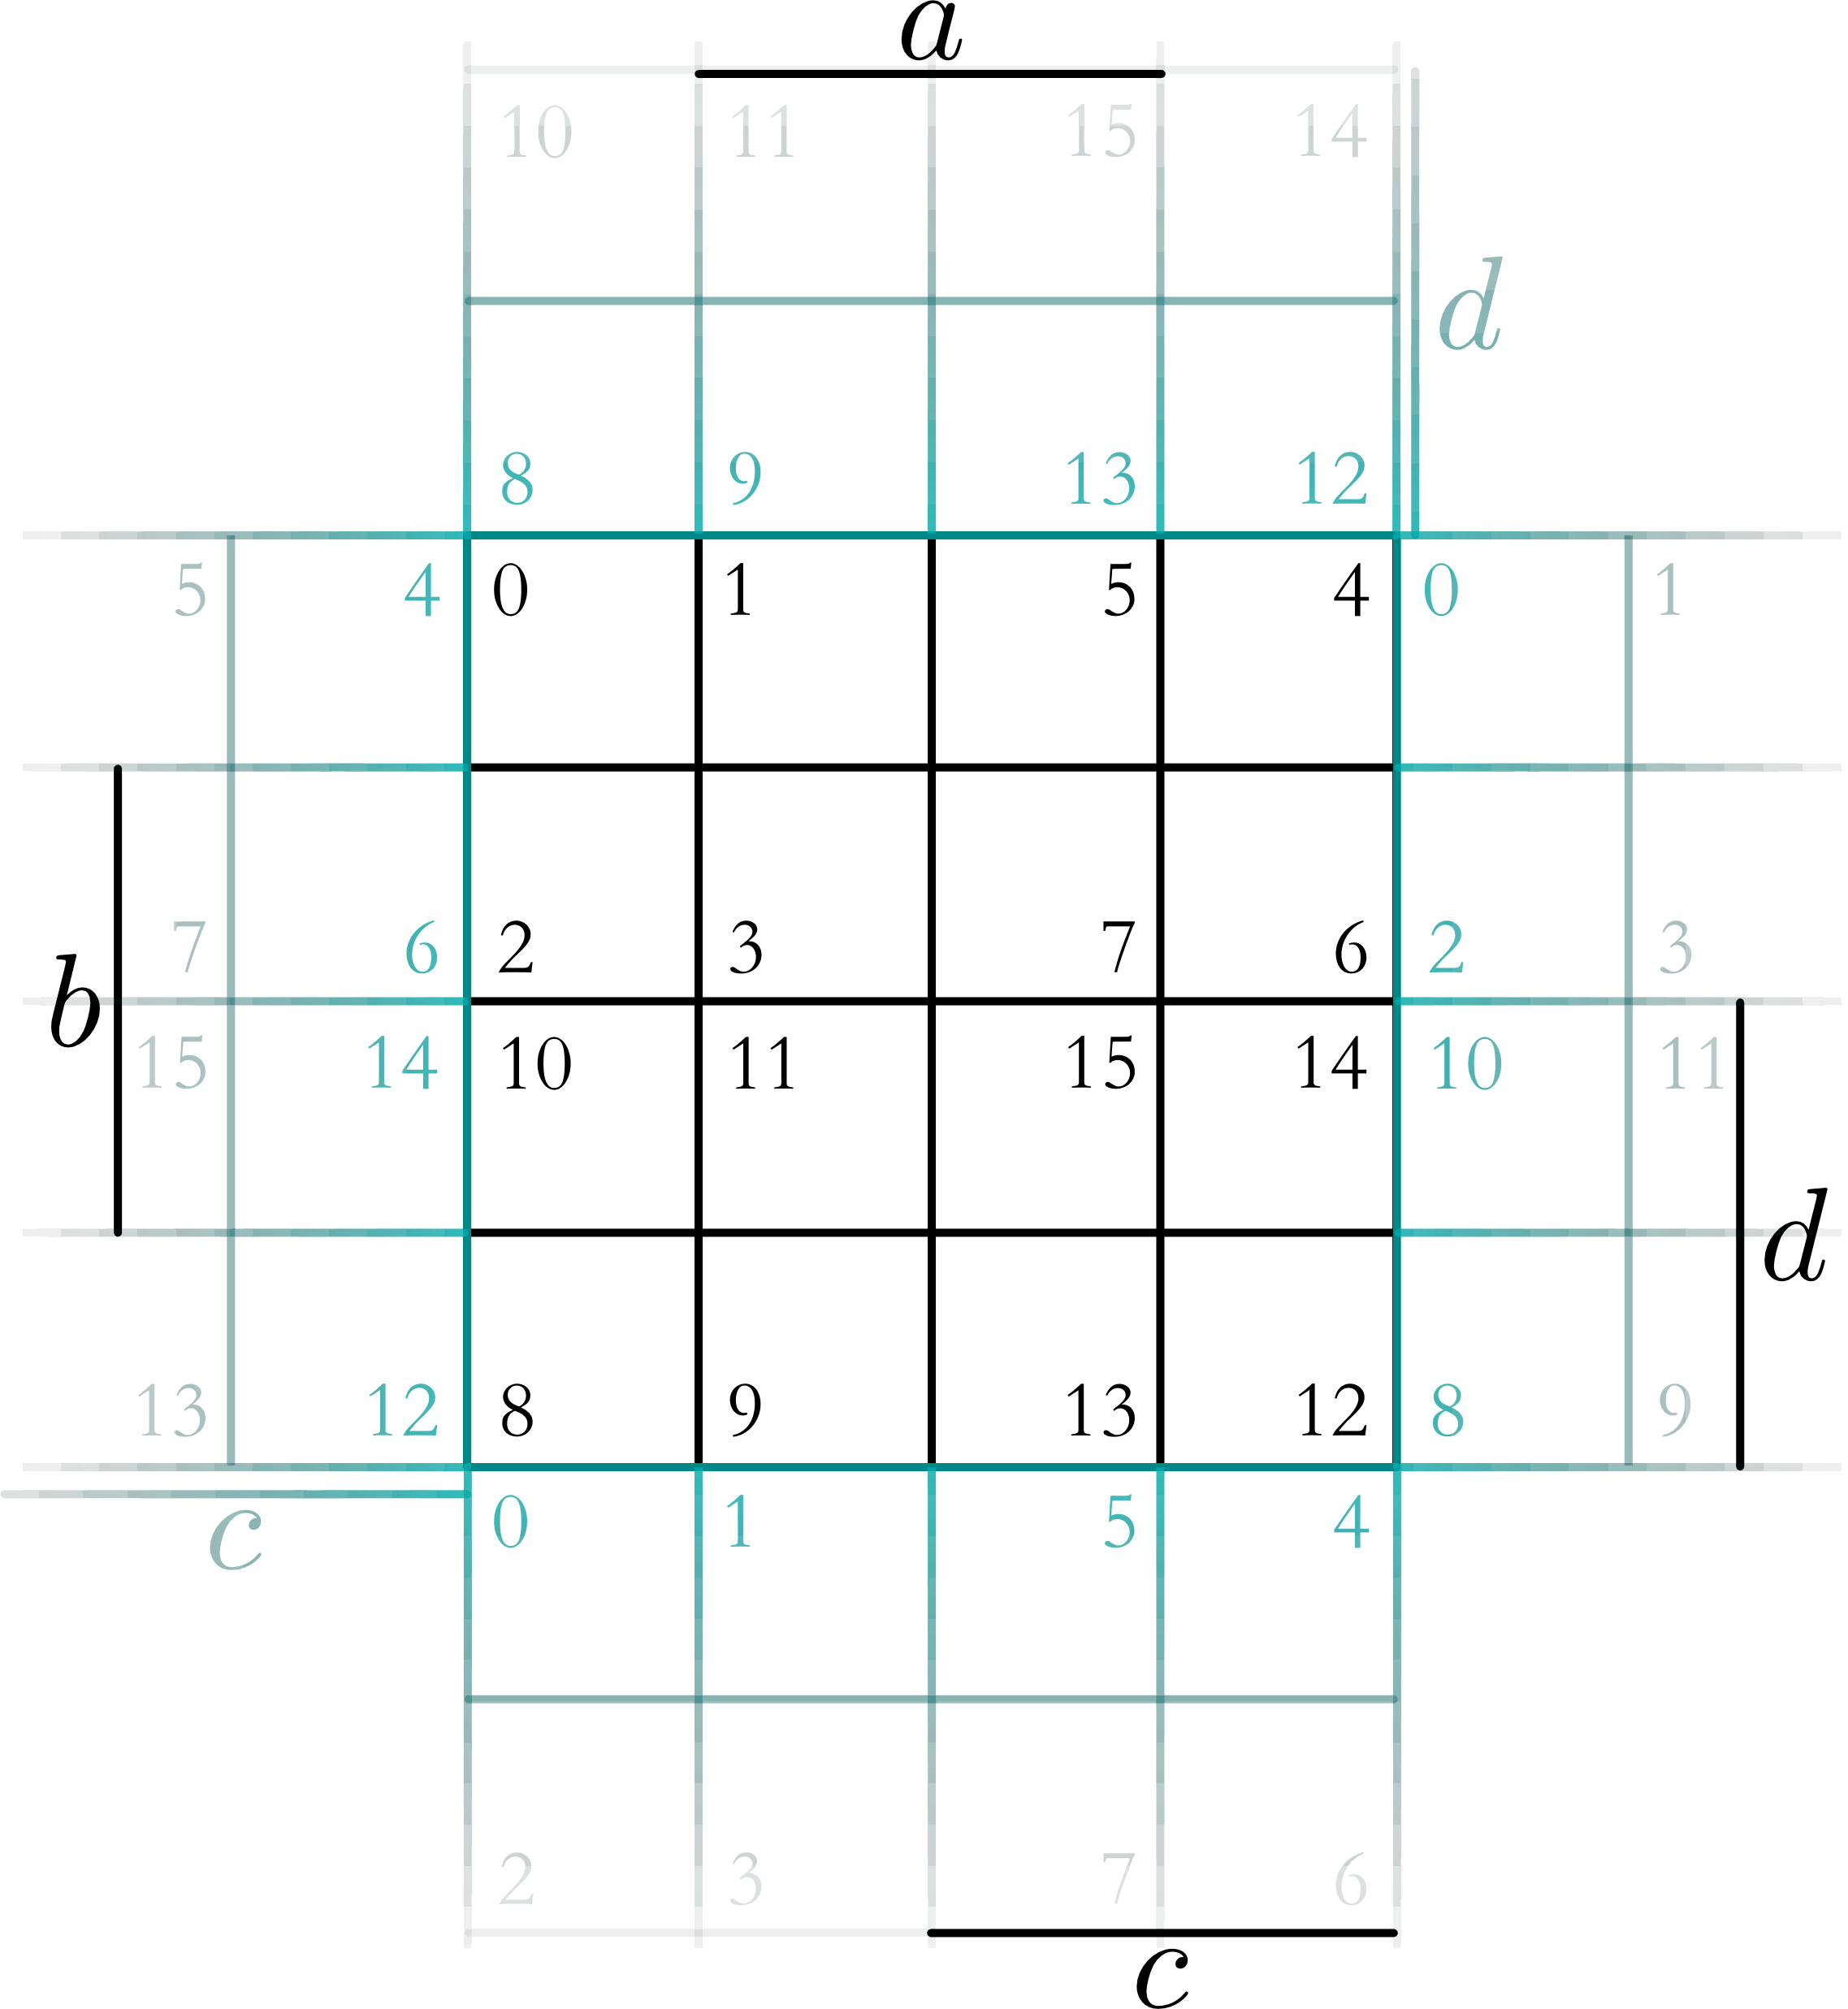
\includegraphics[scale = 0.5]{KV4diagramm_Nachbarschaften.png}
	\caption{durch Aneinanderreihung der Diagramme sind die weniger offensichtlichen Nachbarschaften angedeutet.}
	\label{KVdiag_nachbarschaften}
\end{figure}

Mit Nachbarschafts-Eigenschaft können Funktionen mittels des Diagramms minimiert werden. Laut der zuvor in diesem Abschnitt vorgestellten algebraischen Regeln dürfen sich um eine Minimierung zweier Terme zu ermöglichen die beiden Terme ausschließlich in der Negation einer einzigen Variablen unterscheiden. Da aus den mit dem Wert $1$ belegten Feldern direkt die Minterme resultieren, können diejenigen Minterme zusammengefasst werden, deren Felder benachbart sind. Analog gilt dies für die Maxterme, welche aus den mit $0$ belegten Feldern resultieren. 

Beispiele:
\begin{itemize}
	\item
		Beispiel: Die Funktion $f = ab + a\overline{b}$ soll minimiert werden. Algebraisch kann folgende Vereinfachung vorgenommen werden:
		\begin{align*}
			f &= ab + a\overline{b}  \\
			  &= a(b + \overline{b}) \\
			f &= a                   \\
		\end{align*}
		Die Funktion im KV-Diagramm:
		\begin{center}
			{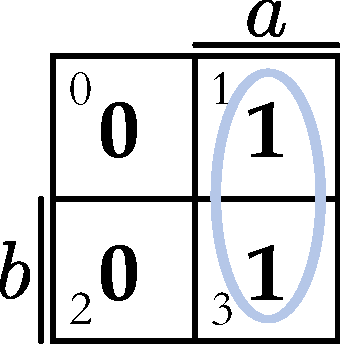
\includegraphics[scale = 0.5]{KV2diagramm_belegt.pdf}}
		\end{center}
		Aus dem Diagramm kann der aus den beiden Mintermen $m_1 = \overline{b}a$ und $m_3 = ba$ der zusammengefasste Term $a$ direkt abgelesen werden. So ergibt sich ebenfalls die minimierte Formel $f = a$ .
	\item
		Beispiel: Die Funktion $f = \overline{b}a + b\overline{a} + ba$ soll minimiert werden. Algebraisch kann folgende Vereinfachung vorgenommen werden:
		\begin{align*}
			f &= \overline{b}a + b\overline{a} + ba  \\
			  &= \overline{b}a + b\overline{a} + ba + ba \\
			  &= \overline{b}a + b(\overline{a} + a) + ba \\
			  &= a(\overline{b} + b) + b(\overline{a} + a) \\
			f &= a + b \\
		\end{align*}
		Die Funktion im KV-Diagramm:
		\begin{center}
			{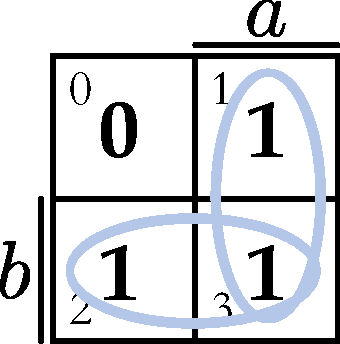
\includegraphics[scale = 0.5]{KV2diagramm_belegt2.pdf}}
		\end{center}
		Aus dem Diagramm kann der aus den beiden Mintermen $m_1 = \overline{b}{a}$ und $m_3 = ba$ der zusammengefasste Term $a$ direkt abgelesen werden. Weiterhin ergibt sich aus den beiden Mintermen $m_2 = {b}\overline{a}$ und $m_3 = ba$ der zusammengefasste Term $b$. So ergibt sich ebenfalls die minimierte Formel $f = b + a$ .
\end{itemize}
%TODO weitere Beispiele hinzufügen

%TODO Def zu Kern- und Primimplikanten ergänzen

Für eine minimale Konjunktive Form wird zuerst die minimale Disjunktive Form der negierten Funktion erstellt. Dies geschieht indem 0en zusammengefasst werden und die zusammengefassten Terme Disjunktiv miteinander verknüpft werden, wie bisher. Um aus der Disjunktiven Form der negierten Funktion zur Konjunktiven Form der Funktion als solche zu kommen muss die erhalgene Disjunktive Form negiert werden. Somit ergibt sich nach De Morgan die minimierte Konjunktive Form der Funktion an sich.

%TODO Beispiele ergänzen
%TODO Begründung für 1er 2er 4er 8er Gruppen einfügen; 2er kickt 1Variable; 4er kickt 2Varbiablen; 8er kickt 3Variablen
\subsubsection*{Vorgehensweise für die Vereinfachung in Disjunktiver Form}
\begin{enumerate}
  \item übertrage die SBT oder die Kanonische Disjunktive Normalform in das KV-Diagramm.
  \item gruppiere alle 1en in insgesamt möglichst wenigen möglichst großen 1er, 2er, 4er oder 8er Gruppen  bis jede 1 abgedeckt ist.
  \item lese den Gruppen entsprechend die reduzierten Terme aus.
  \item verknüpfe die reduzierten Terme disjunktiv und erhalte die minimierte Disjunktive Form.
\end{enumerate}

\subsection{Halb- und Volladdierer}
Die Addition von Dualzahlen kann über logische Funktionen und damit in logischen hardwaretechnischen Schaltungen abgebildet werden. Ein Halbaddierer berechnet die Summe $s$ von zwei Bits $a$ und $b$ mit Berücksichtigung des Übertrags\footnote{Übertrag engl. carry} $c$. Der Volladdierer berücksichtigt in der Eingabe zusätzlich das carry-Bit.

\begin{minipage}[t]{0.5\textwidth} \vspace{0mm} \centering
	\textbf{Halbaddierer SBT}
	
	\begin{tabular}{c*{4}{c}}
		$i$ & 0 & 1 & 2 & 3 \\ \hline
		$a$ & 0 & 1 & 0 & 1 \\
		$b$ & 0 & 0 & 1 & 1 \\ \hline
		$s$ & 0 & 1 & 1 & 1 \\ \hline
		$c$ & 0 & 0 & 0 & 1 \\
	\end{tabular}
	
	$s = a + b$
	
	$c = a \cdot b $
\end{minipage}
\begin{minipage}[t]{0.5\textwidth} \vspace{0mm} \centering
	\textbf{Volladdierer SBT}
	
	\begin{tabular}{c*{8}{c}}
		$i$ & 0 & 1 & 2 & 3 & 4 & 5 & 6 & 7 \\ \hline
		$c$ & 0 & 1 & 0 & 1 & 0 & 1 & 0 & 1 \\
		$b$ & 0 & 0 & 1 & 1 & 0 & 0 & 1 & 1 \\
		$a$ & 0 & 0 & 0 & 0 & 1 & 1 & 1 & 1 \\ \hline
		$s$ & 0 & 1 & 1 & 0 & 1 & 0 & 0 & 1 \\ \hline
		$c$ & 0 & 0 & 0 & 1 & 0 & 1 & 1 & 1 \\
	\end{tabular}
	
	$s_{\textit{DNF}} = \overline{c}\overline{b}a
		+ \overline{c}b\overline{a} 
		+ c\overline{b}\overline{a}
		+ cba$
	
	$c_{\textit{DNF}} = \overline{a}bc
		+ c\overline{b}a 
		+ cb\overline{a}
		+ cba$
\end{minipage}

\chapter{Informationstheorie}
%TODO: Informationen zum Thema Informationstheorie aus ausführlichem Skript dgt_all einarbeiten
In der Informationstheorie geht es um die Definition und quantitative Bewertung von Information. Im Folgenden geht es um den Austausch von Informationen mittels Nachrichten über Kanäle. Ein Kommunikationssystem wird durch die Kommunikationspartner, der Kommunikationsrichtung und der Informationsart charakterisiert. Als Kommunikationsparter können Menschen und Maschinen auftreten.     Die Kommunikationsrichtung wird allgemein mit simplex oder duplex beschrieben. Ist ein Kommunikationskanal simplex aufgebaut, so erfolgt das Senden der Nachrichten immer vom selben Kommunikationsteilnehmer. Als duplex werden Kommunikationskanäle bezeichnet über die beide Kommunikationspartner gleichzeitig einander Nachrichten senden und empfangen. Zusätzlich gibt es die Bezeichnung halb-duplex, damit ist gemeint, dass nicht gleichzeitig gesendet und empfangen werden kann, sondern die beiden Kommunikationspartner sich mit senden und empfangen von Nachrichten abwechseln. Die Art der Information kann beispielsweise in Daten oder Befehle klassifiziert werden.

Die Information einer Nachricht ist nur dann von Bedeutung, wenn der Empfänger daraus etwas ihm bislang unbekanntes erfährt. Im Fall von Befehlen kann dies zusätzlich zu einer Änderung von Verhaltensweisen führen. Bei der Analyse von Nachrichten wird in drei Betrachtungsweisen unterschieden:
\begin{itemize}
  \item \textbf{Syntax} ist die äußere Form in Form von Zeichen und grammatikalischer Regeln der Sprache in der die Nachricht verfasst ist. Hierbei kann die mathematische Formulierung und quantitative Bewertung untersucht werden.
  \item \textbf{Semantik} ist die Bedeutung und Sinn der Nachricht.
  \item \textbf{Pragmatik} ist die Untersuchung der Auswirkung der Information auf das Verhalten des Empfängers.
\end{itemize}

Die Informationstheorie befasst sich ausschließlich mit der Syntax. In den folgenden Abschnitten wird näher auf die formale Beschreibung und quantitative Bewertung von Übertragungskanälen eingegangen. Abschließend werden geeignete Codierungsverfahren vorgestellt, die sich aus neuen Erkenntnissen im Hinblick auf Optimierung erschließen.

\section{Begriffe}
%TODO Begriffsdefinitionen ergänzen

\section{Informationsquellen}
Digitale Informationsquellen\footnote{Digitale Informaitonsquellen = Diskrete Informationsquellen} bilden Nachrichten mit Zeichen aus einem Alphabet. Die Informationserzeugung ist aus Sicht des Empfängers ein stochastischer Prozess. Dabei kann die Wahrscheinlichkeit, dass ein bestimmtes Zeichen gesendet wird von vorn herein angegeben werden. Damit kann eine Quelle mit $n$ unterschiedlichen Zeichen $a_i$ aus dem Alphabet $A = \{a_i \mid i \in \{1, \ldots, n\}\}$ und der Wahrscheinlichkeit $P(a_i)$, dass das Zeichen $a_i$ gesendet wird, mit folgendem \textit{Wahrscheinlichkeitsfeld} beschrieben werden:
$$
	X =
	\left(
		\begin{array}{*{4}{c}}
		  a_1    &  a_2   &  a_3   \\
		  P(a_1) & P(a_2) & P(a_3) \\
		\end{array}
	\right)
$$

Da beim Senden genau alle Zeichen des Alphabetes zur Auswahl stehen ist die Summe aller Zeichenwahrscheinlichkeiten $1$.
$$
	\sum_{i=1}^n P(a_i) = 1
$$

Eine \textit{stationäre Quelle} charakterisiert eine Quelle als zeitunabhängig. Das heißt über alle Zeitpunkte hinweg ist die Zeichenwahrscheinlichkeit eines jeden Zeichens konstant.

Quellen ohne Gedächtnis werden als unabhängige Quellen bezeichnet. Dabei gilt, dass die Wahrscheinlichkeit eines Zeichens unabhängig von jedem anderen Zeichen zu betrachten ist. Für die Wahrscheinlichkeit, dass ein Zeichen $a_j$ auf das Zeichen $a_i$ folgt gilt dabei:
$$ P(a_i, a_j) = P(a_i) \cdot P(a_j) $$

\subsection{Entscheidbarkeit und Entropie von Quellen}
Die absolute Entscheidbarkeit einer Quelle ist abzulesen an der Anzahl Entscheidungsfragen\footnote{wikipedia: "`Die Entscheidungsfrage (auch: Ja/nein-Frage, Satzfrage) ist ein Typ von Fragesatz. Entscheidungsfragen sind die Fragen, auf die man nur mit ja oder mit nein antworten kann."'}, die gestellt werden müssen um ein gesendetes Zeichen zu erfragen. Für die absolute Entscheidbarkeit $H_0(X)$ von einer Quelle $X$, deren Alphabet $n$ unterschiedlichen Zeichen hat, gilt:
%TODO Beispiel zum Erfragen eines Zeichens einfügen
$$ H_0(X) = ld(n) $$

Der Informationsgehalt einer Quelle wird durch die Entropie bestimmt. Die Entropie der Quelle lässt sich mit dem Informationsgehalt eines jeden Zeichns berechnen. Der Informationsgehalt $H(a_i)$ eines Zeichens $a_i$ ist:
$$ 
	H(a_i) = ld \left( \frac{1}{P(a_i)} \right) \left[ \frac{bit}{Zeichen} \right]
$$

Hinweis: wegen $0 < P(a_i) \le 1$ gilt $\frac{1}{P(a_i)} \ge 1$ und $H(a_i) \ge 0$ \\
Die Definition des Informationsgehaltes eines Zeichens $H(a_i)$ ist praktisch anwendbar, da damit die Zeichenwahrscheinlichkeit berücksichtigt wird. Der Logarithmus wird wegen der Entscheidbarkeit gezogen.

Die Entropie einer Quelle ist definiert mit:
\begin{align*}
	H(X) &= P(a_1) \cdot H(a_1) + P(a_2) \cdot H(a_2) + \ldots + P(a_n) \cdot H(a_n) \\
	     &= \sum_{i=1}^n P(a_i) \cdot H(a_i) \\
	     &= \sum_{i=1}^n P(a_i) \cdot ld \left( \frac{1}{P(a_i)} \right) \left[ \frac{bit}{Zeichen} \right]\\
\end{align*}

So ergibt sich für eine Quelle $G$ mit gleichwahrscheinlichen Zeichen, dass die Entropie gleich der absoluten Entscheidbarkeit ist.
\begin{align*}
	H(G) &= \sum_{i=1}^n P(a_i) \cdot ld \left( \frac{1}{P(a_i)} \right) \\
	     & \textnormal{wegen } P(a_i) = P(a_j) = \frac{1}{n} \textnormal{ gilt:} \\
	     &= \sum_{i=1}^n \frac{1}{n} \cdot ld \left( \frac{1}{\frac{1}{n}} \right) \\
	     &= n \cdot \left( \frac{1}{n} \cdot ld \left( \frac{1}{\frac{1}{n}} \right) \right)\\
	     &= \frac{n}{n} \cdot ld(n) \\
	H(G) &= ld(n) = H_0(G) \left[ \frac{bit}{Zeichen} \right]\\
\end{align*}

Wenn eine Quelle Zeichen mit unterschiedlicher Wahrscheinlichkeit erzeugt lässt sich im Bezug auf die Entropie und die absolute Entscheidbarkeit eine Redundanz feststellen. Die absolute Redundanz $R$ wird berechnet mit:
$$
	R = H_0 - H \left[ \frac{bit}{Zeichen} \right]
$$
Die relatve Redundanz $r$ wird ergibt sich aus:
$$
	r = \frac{R}{H_0} = \frac{H_0 - H}{H_0}
$$

%TODO ergänzen: Abschnitt über Eigenschaften der Entropie

\subsubsection*{Entropie von Verbundquellen}
Eine Quelle kann aus mehreren anderen Quellen zusammengesetzt sein. Das Alphabet der Verbundquelle kann als kartesisches Produkt der Alphabete der Einzelquellen aufgefasst werden. Wird eine Verbundquelle aus einer Quelle mit dem Alphabet $A$ und einer anderen mit dem Alphabet $B$ in dieser Reihenfolge gebildet so gilt für das Alphabet $C$ der Verbundquelle:
\begin{align*}
	C &= A \times B \\
	  &= \{a_1, a_2, \ldots, a_n\} \times \{b_1, b_2, \ldots, b_m\} \\
	  &= \{(a_1,b_1), (a_1,b_2), \ldots, (a_1,b_m), \ldots, (a_n,b_m) \}\\
\end{align*}
Dieses Prinzip kann für $k$ viele Teilquellen verallgemeinert werden:
$$ C = A_1 \times A_1 \times A_1 \times \ldots \times A_k $$ 

Handelt es sich bei der Verbundquelle um eine unabhängige Verbindung der Teilquellen so wird jede Kombination von Zeichen gleichwahrscheinlich generiert. Wird eine Verbundquelle $Z$ aus einer Quelle $X$ mit dem Alphabet $A$ der Länge $n$ und einer anderen Quelle $Y$ mit dem Alphabet $B$ der Länge $m$ in dieser Reihenfolge gebildet so gilt für die Wahrscheinlichkeitsfelder der Teilquellen $X$ und $Y$, wie bisher:
$$
	X =
	\left(
		\begin{array}{*{5}{c}}
		  a_1    &  a_2   & \ldots &  a_n   \\
		  P(a_1) & P(a_2) & \ldots & P(a_n) \\
		\end{array}
	\right)
$$
$$
	X =
	\left(
		\begin{array}{*{5}{c}}
		  b_1    &  b_2   & \ldots &  b_m   \\
		  P(b_1) & P(b_2) & \ldots & P(b_m) \\
		\end{array}
	\right)
$$
Für das Wahrscheinlichkeitsfeld der Verbundquelle $Z = X \times Y$ ergibt sich demnach:
$$
	X =
	\left(
		\begin{array}{*{5}{c}}
		  a_1b_1    &  a_1b_2   & \ldots &  a_nb_m   \\
		  P(a_1, b_1) & P(a_1, b_2) & \ldots & P(a_n, b_m) \\
		\end{array}
	\right)
$$

Die Entropie der Verbundquelle ist also:
\begin{align*}
	H(Z) &= H(X,Y) \\
	H(Z) &= \sum_{i = 1}^n \sum_{j = 1}^m P(x_i,y_j) 
	     	\cdot ld \left( \frac{1}{P(x_i,x_j)} \right) \\
	     & \textnormal{dies lässt sich vereinfachen:} \\
	     &= \sum_{i = 1}^n \sum_{j = 1}^m P(x_i) \cdot P(y_j) 
	     	\cdot ld \left( \frac{1}{P(x_i)\cdot P(x_j)} \right) \\
	     &= \sum_{i = 1}^n \sum_{j = 1}^m P(x_i) \cdot P(y_j) 
	     	\cdot \left( ld \left( \frac{1}{P(x_i)} \right) 
	     	+ ld \left( \frac{1}{P(x_j)} \right) \right) \\
	     &= \sum_{i = 1}^n \sum_{j = 1}^m P(x_i) \cdot P(y_j) 
	     	\cdot ld \left( \frac{1}{P(x_i)} \right) 
	     	+ P(x_i) \cdot P(y_j) 
	     	\cdot ld \left( \frac{1}{P(x_j)} \right) \\
	     &= \sum_{i = 1}^n \sum_{j = 1}^m P(x_i) \cdot P(y_j) 
	     	\cdot ld \left( \frac{1}{P(x_i)} \right) 
	     	+ \sum_{i = 1}^n \sum_{j = 1}^m P(x_i) \cdot P(y_j) 
	     	\cdot ld \left( \frac{1}{P(x_j)} \right) \\
	     &= \sum_{i = 1}^n P(x_i) \cdot ld \left( \frac{1}{P(x_i)} \right) 
	     	\cdot \sum_{j = 1}^m P(y_j)
	     	+ \sum_{j = 1}^m P(y_j) \cdot ld \left( \frac{1}{P(x_j)} \right)
	     	\cdot \sum_{i = 1}^n P(x_i) \\
	     & \textnormal{wegen } \sum_{j = 1}^m P(y_j) = 1 \textnormal{ und } 
	     	\sum_{i = 1}^m P(x_i) = 1 \\
	     &= \sum_{i = 1}^n P(x_i) \cdot ld \left( \frac{1}{P(x_i)} \right)
	     	+ \sum_{j = 1}^m P(y_j) \cdot ld \left( \frac{1}{P(x_j)} \right) \\
	H(Z) &= H(X,Y) = H(X) + H(Y) \\     
\end{align*}

Allgemein für Verbundquellen mit k vielen unabhängigen Teilquellen gilt:
\begin{align*}
	H(X_1, X_2, \ldots, X_k) &= 
		\sum_{i_1 = 1}^{n_1} \sum_{i_2 = 2}^{n_1} \ldots \sum_{i_k = 1}^{n_k}
		P(a_1i_1, a_2i_2, \ldots, a_ki_k) 
		\cdot ld \left( \frac{1}{P(a_1i_1, a_2i_2, \ldots, a_ki_k)} \right) \\
		&= H(X_1) + H(X_2) + \ldots + H(X_k)
\end{align*}
 
%TODO: Erläuterung zu abhängigen Quellen und abhängigen Teilquellen ergänzen
%TODO: Thema Informationsfluss ergänzen

\subsection{Informationsübertragung}
Um allgemein die Informationsübertragung zu betrachten sehen wir die Informations-Quelle und Informations-Senke als neutraler Beobachter. Dabei wird die Informations-Senke ebenfalls als Quelle betrachtet, da sich auf dem Übertragungskanal wegen auftretender Störungen Nachrichten der Ursprünglichen Quelle verändert werden können. Der Übertragungskanal kann aus Perspektive des Beobachters wie eine Verbundquelle aus Informations-Quelle und Informations-Senke betrachtet werden.
\begin{figure}[htbp] % positioning htbp: h = here; t = top; b bottom; p own page
	\centering
	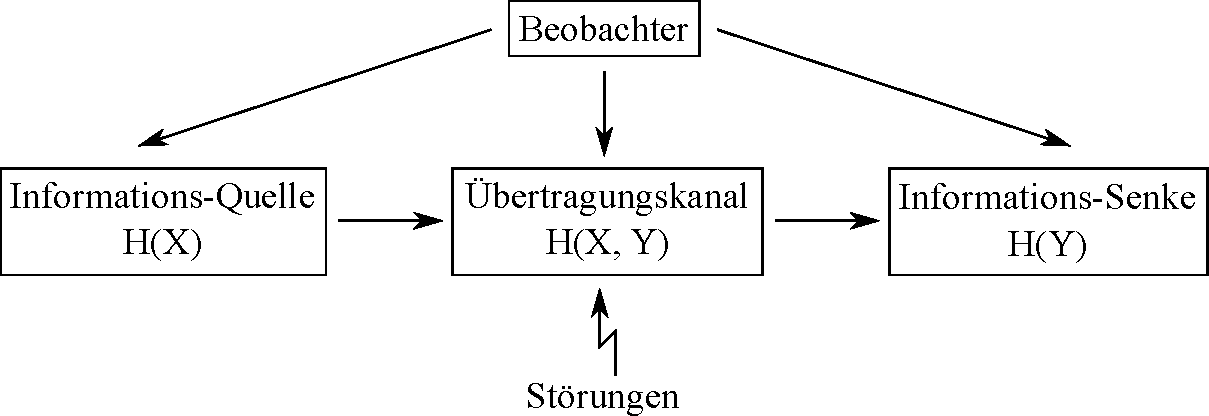
\includegraphics[width=0.8\textwidth]{informationsuebertragung.pdf}
	\caption{Betrachtung der Informationsübertragung als neutraler Beobachter}
	\label{iübertragung}
\end{figure}

Bei einer störungsfreien Übertragung gilt müssen die Entropien aller im Modell als Quellen betrachteten Informationsträger gleich sein. 
$$H(X,Y) = H(X) = H(Y)$$
Abbildung \ref{hxEQhy} zeigt die Beziehung der Entropien im Diagramm.

\begin{figure}[htbp] % positioning htbp: h = here; t = top; b bottom; p own page
	\centering
	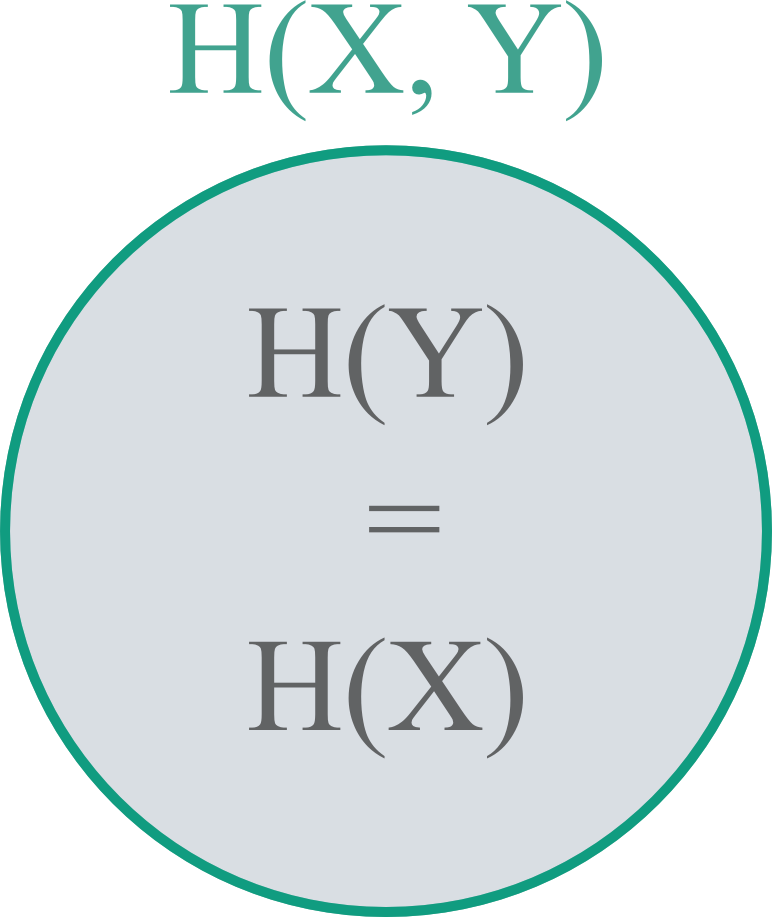
\includegraphics[scale=0.4]{HXgleichHY.png}
	\caption{$H(X)$ gleich $H(Y)$ und damit auch gleich $H(X,Y)$}
	\label{hxEQhy}
\end{figure}

Bei einer vollständig gestörten Übertragung erhält die Informations-Senke völlig andere Informationen als ursprünglich gesendet wurden. Der Beobachter sieht zwei unabhängige Informationsquelen. In diesem Fall ist die Entropie des Übertragungskanals als Verbundquelle maximal und es gilt
$$H(X,Y) = H(X) + H(Y)$$
Abbildung \ref{hxymax} zeigt die Beziehung der Entropien im Diagramm.

\begin{figure}[htbp] % positioning htbp: h = here; t = top; b bottom; p own page
	\centering
	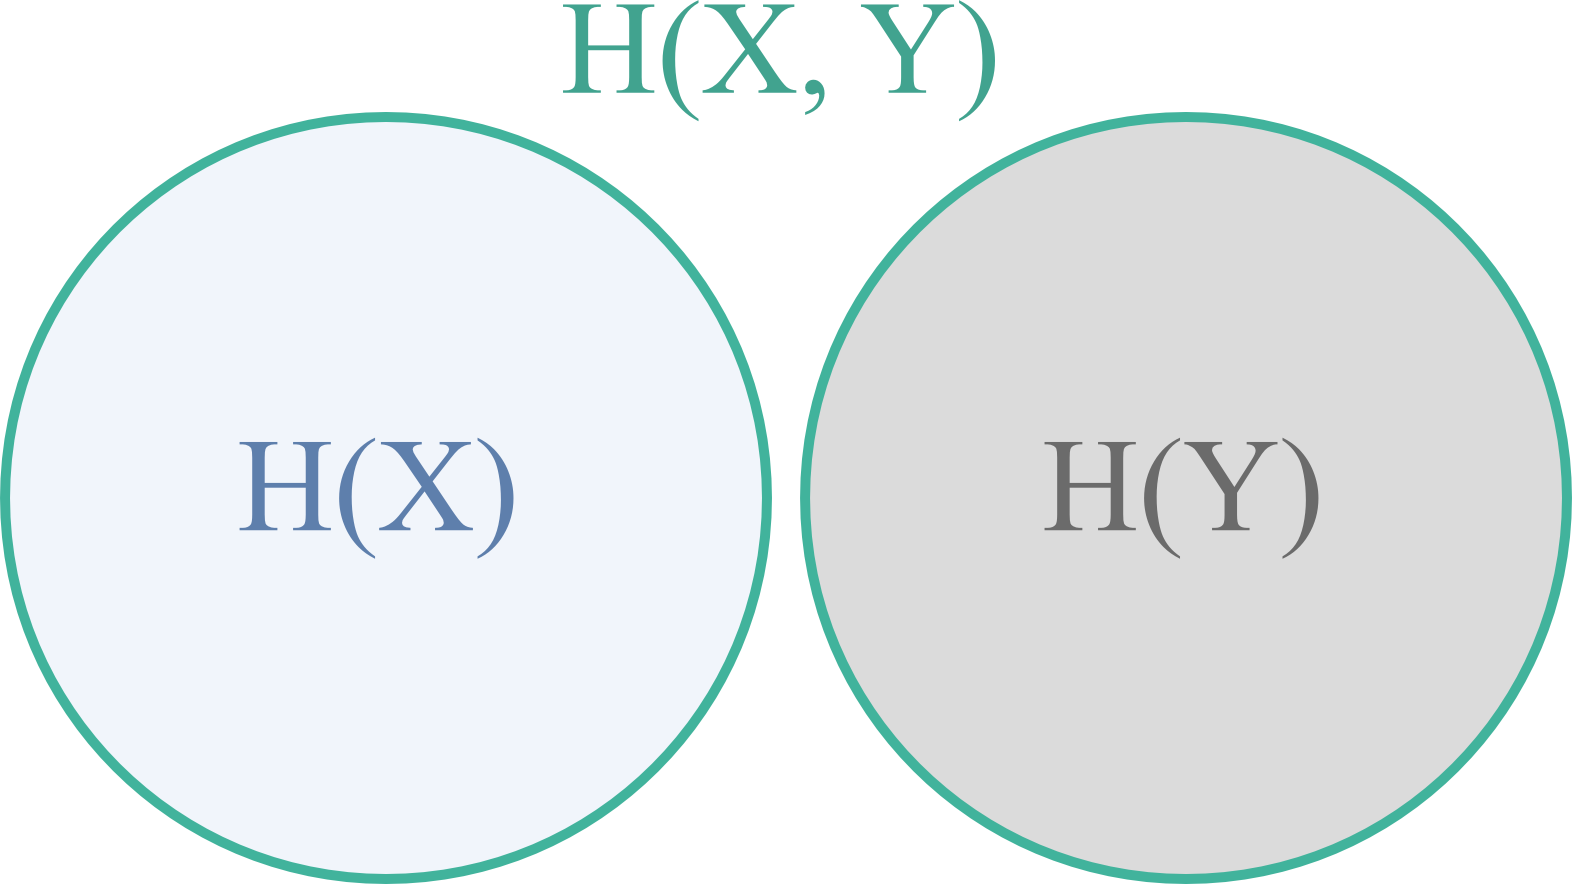
\includegraphics[scale=0.4]{HXYmax.png}
	\caption{$H(X,Y)$ ist maximal}
	\label{hxymax}
\end{figure}

Allgemein schwankt die Entropie der Verbundquelle zwischen maximalem und minimalem Wert je nachdem wie stark die Störungen ausfallen.
$$ H(X) \le H(X,Y) \le H(X) + H(Y) $$
Abbildung \ref{hxymid} zeigt die Beziehung der Entropien im Diagramm.
\begin{figure}[htbp] % positioning htbp: h = here; t = top; b bottom; p own page
	\centering
	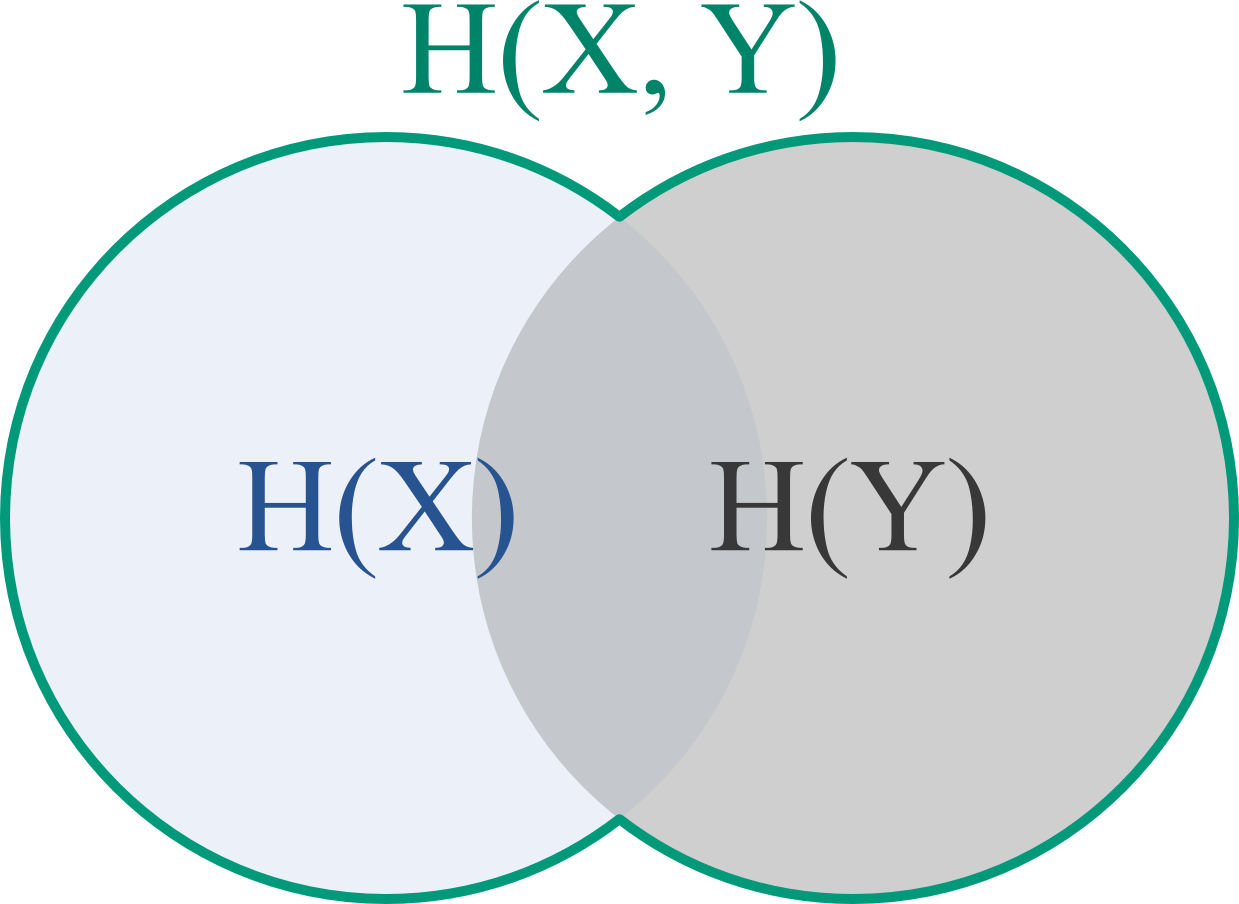
\includegraphics[scale=0.4]{HXYmiddle.png}
	\caption{$H(X,Y)$ zwischen maximalem und minimalem Wert}
	\label{hxymid}
\end{figure}

Die bei der Übertragung verloren gegangene Quellinformation wird \textsl{Äquivokation} genannt. Deren Entropie wird mit $H(X \backslash Y)$ bezeichnet.\footnote{$H(X \backslash Y)$ lies "`Entropie von X ohne Y"'} Die Entropie der Äquivokation lässt sich berechnen mit:
$$ H(X \backslash Y) = H(X, Y) - H(Y) $$

Information, die bei der Übertragung durch Störungen hinzu gefügt wurde, wird \textit{Irrelevanz} genannt. Die Bezeichnung der Entropie der Irrelevanz ist $H(Y \backslash X)$ und wird wie folgt berechnet:
$$H(Y \backslash X) = H(X, Y) - H(X)$$

Die \textsl{Transinformation} ist die Information, welche von der Quelle an den Empfänger tatsächlich übertragen wurde. Die Tansinformation ist die Schnittmenge der Quellinformation mit der empfangenen Information. Die Entropie der Transinformation wird mit $H(X;Y)$ bezeichnet und wie folgt berechnet: 
\begin{align*}
	H(X;Y) &= H(X,Y) - H(X \backslash Y) 
		- H(Y \backslash X) \\
	       &= H(X) + H(Y) - H(X,Y)
\end{align*}

%TODO Kanalkapazität ergänzen

Die Abbildungen \ref{infokanal} und \ref{teilinfo} veranschaulichen die Begriffe Äquivokation, Transinformation und Irrelevanz.
\begin{figure}[htbp] % positioning htbp: h = here; t = top; b bottom; p own page
	\centering
	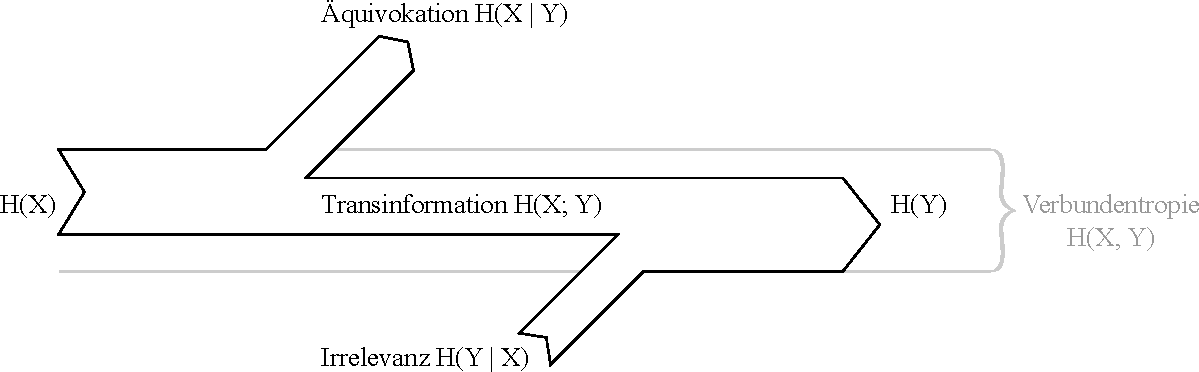
\includegraphics[width = 0.9\textwidth]{informationskanal.pdf}
	\caption{Betrachtung des Informationskanals mit entsprechenden Teilinformationen Äquivokation, Transinformation und Irrelevanz}
	\label{infokanal}
\end{figure}
\begin{figure}[htbp] % positioning htbp: h = here; t = top; b bottom; p own page
	\centering
	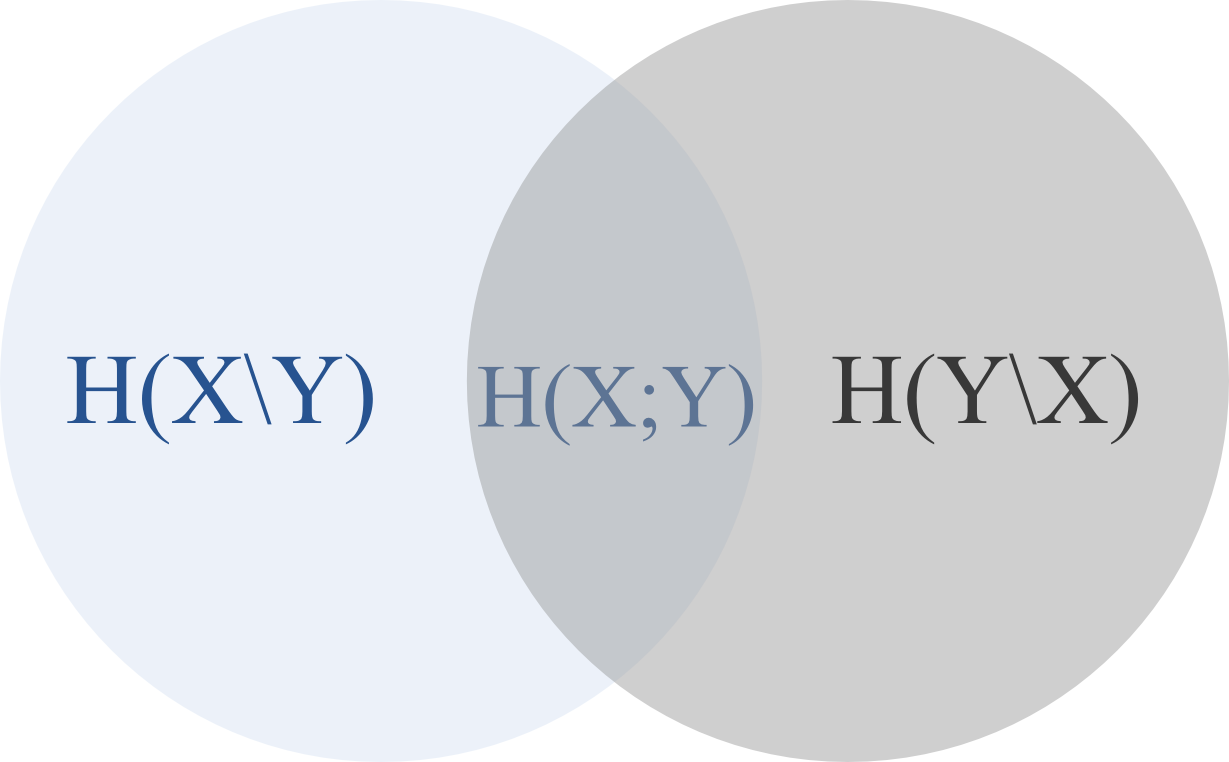
\includegraphics[scale=0.4]{teilinformation.png}
	\caption{Beziehungen der Entropien der Teilinformationen}
	\label{teilinfo}
\end{figure}

%TODO Informationsübertragung Sonderfälle ergänzen

\newpage
\section{Gestörte Übertragungskanäle}
In diesem Abschnitt wird am Beispiel eines symmetrisch gestörten Übertragungskanals die Analyse der Entropien durchgeführt. Es wird eine Quelle $X$ mit dem Binäralphabet $A = \{a_1,a_2\}$ betrachtet. Die Quelle $X$ und die Senke $Y$ mit dem Alphabet $B = \{b_1, b_2\}$ sind über folgende Wahrscheinlichkeitsfelder allgemein definiert:
$$
	X =
	\left(
	\begin{array}{cc}
		a_1    & a_2 \\
		P(a_1) & 1-P(a_1)
	\end{array}
	\right)
	\hspace{1cm}
	Y = 
	\left(
	\begin{array}{cc}
		b_1    & b_2 \\
		P(b_1) & 1-P(b_1)
	\end{array}
	\right)
$$

Bei Fehlerfreier Übertragung entspricht das Zeichen $a_1$ dem Zeichen $b_1$ und $a_2$ entspricht $b_2$. Die Wahrscheinlichkeit, dass ein Zeichen einem falschen Zeichen zugeordnet wird, weil es sich hier um Binäralphabete handelt, Bitfehlerwahrscheinlichkeit $P_f$ genannt. Dass statt $a_1$ $b_2$ beim Empfänger empfangen wird geschieht mit Wahrscheinlichkeit $P(a_1 \mid b_2)$. Die Bezeichnung $P(a_1 \mid b_2)$ beschreibt das Ereignis, dass bei der Übertragung $a_1$ gesendet und $b_2$ empfangen wird. Entsprechend gilt für $P(a_1 \mid b_1)$ die Wahrscheinlichkeit, dass wenn $a_1$ gesendet wird auch $b_1$ empfangen wird. Da die Bitfehlerwahrscheinlichkeit in diesem Beispiel symmetrisch ist gilt:
$$ P(a_1 \mid b_2) = P(a_2 \mid b_1) = P_f $$

Das die unterschiedlichen Ereignisse im Diagramm dargestellt zeigt Abbildung \ref{symStoerung}. Die Pfeile zeigen mit ihrer Beschriftung, wie die Wahrscheinlichkeiten bezeichnet werden und wie diese in diesem Beispiel zusammenhängen. 
\begin{figure}[htbp] % positioning htbp: h = here; t = top; b bottom; p own page
	\centering
	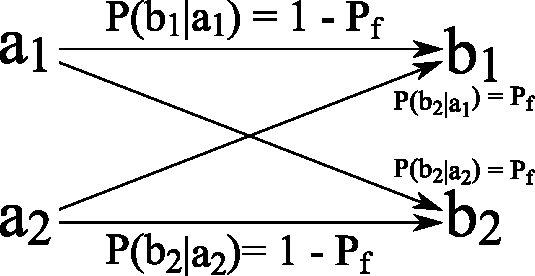
\includegraphics[scale=.8]{symmetrischeStoerung.pdf}
	\caption{Wahrscheinlichkeiten bei der Übertragung der Zeichen}
	\label{symStoerung}
\end{figure}
Im folgenden wird das Wahrscheinlichkeitsfeld der Verbundquelle erstellt, also der Quelle in der wir Infermationserzeuger und -Empfänger gemeinsam betrachten. Jede Wahrscheinlichkeit eines Ereignisses berechnet sich aus der Wahrscheinlichkeit, dass die Quelle ein bestimmtes Zeichen sendet und der Wahrscheinlichkeit, dass dieses Zeichen als solches empfangen oder verfälscht wird. Für das Zeichen $a_1$ werden so die Wahrscheinlichkeiten der beiden Ereignisse berechnet, dass entweder das Zeichen $b_1$ oder das Zeichen $b_2$ empfangen wird. Es gibt also folgende vier Ereignisse:
\begin{center}
	\begin{tabular}{cc}
		$a_1$ wird gesendet und $b_1$ empfangen & $P(a_1) \cdot P(b_1 \mid P(a_1))$ \\
		$a_1$ wird gesendet und $b_2$ empfangen & $P(a_1) \cdot P(b_2 \mid P(a_1))$ \\
		$a_2$ wird gesendet und $b_2$ empfangen & $P(a_2) \cdot P(b_2 \mid P(a_2))$ \\
		$a_2$ wird gesendet und $b_1$ empfangen & $P(a_2) \cdot P(b_1 \mid P(a_2))$ \\ 
	\end{tabular}
\end{center}

Als Beobachter gilt für den Kanal $K$ also das Wahrscheinlichkeitsfeld:
$$
	K = 
	\left(
	\begin{array}{*{4}{c}}
		a_1b_1                          & a_2b_2           & a_1b_2                    & a_2b_1 \\
		P(a_1) P(b_1 \mid P(a_1)) & P(a_2) P(b_2 \mid a_2) & P(a_1) P(b_2 \mid P(a_1)) & P(a_2) P(b_1 \mid P(a_2)) \\
	\end{array}
	\right)
$$

%TODO Rauschmatrix Ü?

Das Wahrscheinlichkeitsfeld kann auch als Verbundmatrix $V$ geschrieben werden:
\begin{align*}
	V &= \left(
	     \begin{array}{*{2}{c}}
	     	P(a_1,b_1) & P(a_1,b_2) \\
	     	P(a_2,b_1) & P(a_2,b_2) \\
	     \end{array}
	     \right) \\
	  &= \left(
	     \begin{array}{*{2}{c}}
	     	P(a_1) P(b_1 \mid P(a_1)) & P(a_1) P(b_2 \mid P(a_1)) \\
	     	P(a_2) P(b_1 \mid P(a_2)) & P(a_2) P(b_2 \mid P(a_2)) \\
	     \end{array}
	     \right) \\
\end{align*}

Aus der Vernundmatrix lassen sich die Wahrscheinlichkeiten der Quellenzeichen über die Summe der Zeilen rückberechnen. Dies gilt, da die Ereignisse je Spalte alle dem Ereignis, dass ein bestimmtest Zeichen gesendet wurde, zuzuordnen sind. Ebenso gilt, dass die Wahrscheinlichkeiten für die empfangenen Zeichen sich über die Summe der jeweiligen Spalten ergeben.

Die Entropie einer Quelle ist maximal, wenn jedes Zeichen des Alphabetes gleich wahrscheinlich generiert werden. Für die Quelle wird die maximale Entropie $H(X) = 1$ angenommen. Also muss $P(a_1) = \frac{1}{2}$ und $P(a_2) = \frac{1}{2}$ gelten. Da die Störungen symmetrisch wirken muss auch $P(b_1) = \frac{1}{2}$ und $P(b_2) = \frac{1}{2}$ gelten. Damit ergibt sich für die Verbundmatrix:

$$
V = 
\left(
\begin{array}{*{2}{c}}
 	\frac{1-P_f}{2} & \frac{P_f}{2} \\
 	\\
 	\frac{P_f}{2}   & \frac{1-P_f}{2} \\
\end{array}
\right)
$$

Die Verbundentropie $H(X,Y)$ ist in diesem Beispiel also:
\begin{align*}
	H(X,Y) &= \sum_{i=1}^2\sum_{j=1}^2
		P(a_i,b_j) \cdot ld \left( 
		\frac{1}{P(a_i,b_j)} \right) \\
		   &= 2 \cdot \frac{1-P_f}{2} 
		\cdot ld \left( 
		\frac{2}{1-P_f} \right) 
		+ 2 \cdot \frac{P_f}{2} 
		\cdot ld \left( 
		\frac{2}{P_f} \right)\\
		   &= (1-P_f) \cdot ld \left( 
		\frac{2}{1-P_f} \right) 
		+ P_f	\cdot ld \left( 
		\frac{2}{P_f} \right)\\
		   &= (1-P_f) \cdot (ld(2) - ld(1-P_f)) 
		+ P_f	\cdot (ld(2) - ld(P_f))\\
		   &= (1-P_f) \cdot (1 - ld(1-P_f)) 
		+ P_f	\cdot (1 - ld(P_f))\\
		   &= (1 - P_f) - (1 - P_f)ld(1-P_f) 
		+ P_f - P_fld(P_f)\\
		   &= 1 - (1 - P_f)ld(1-P_f) - P_fld(P_f)\\
\end{align*}

Die Transinformation ergibt sich aus:
\begin{align*}
	H(X;Y) &= H(X) + H(Y) - H(X,Y) \\
	       &= 1 + 1 - (1 - (1 - P_f)
	       ld(1-P_f) - P_fld(P_f))\\
	       &= 1 + 1 - 1 + (1 - P_f)
	       ld(1-P_f) + P_fld(P_f))\\
	       &= 1 + (1 - P_f)
	       ld(1-P_f) + P_fld(P_f))\\
\end{align*}

Für die Äquivokation folgt:
\begin{align*}
	H(X \backslash Y) &= H(X, Y) - H(Y) \\
	&= 1 - (1 - P_f)ld(1-P_f) 
	- P_fld(P_f) - 1\\
	&= -(1 - P_f)ld(1-P_f) - P_fld(P_f) \\
\end{align*}

Für die Irrelevanz gilt:
\begin{align*}
	H(Y \backslash X) &= H(X, Y) - H(X) \\
	&= 1 - (1 - P_f)ld(1-P_f) 
	- P_fld(P_f) - 1\\
	&= -(1 - P_f)ld(1-P_f) - P_fld(P_f) \\
\end{align*}

Praktischer Weise ist die Transinformation für $P_f = 1$ und $P_f = 0$ maximal. Dies ist sinnvoll, da bei völliger Störung ($P_f = 1$) jedes Bit invertiert wird. Um die ursprüngliche Information zu erhalten reicht es das Bitmuster zu invertieren.

%TODO Optimalcodes / Quellencodierung Einführung ergänzen
%TODO Aufbau von Optimalcodes und Kraft Ungleichung ergänzen
%TODO Shannon-Code ergänzen (nicht klausurrelevant)

\section{Konstruktion von binären Optimalcodes}
\subsection{Fano-Code}
Konstruktionsmethode:
\begin{enumerate}
\item Sortiere abfallend die zu codierenden Zeichen nach deren Wahrscheinlichkeiten.
\item Teile die Gruppe der Zeichen in zwei Gruppen, wobei die Summe der Wahrscheinlichkeiten der einen Gruppe möglichst der Summe der Wahrscheinlichkeiten der anderen Gruppe entspricht. Einer Gruppe wird die $0$ der anderen die $1$ als erste Stelle im Codewort zugeordnet.
\item Wiederhole Schritt 2 mit den entstandenen Teilgruppen, wenn die jeweilige Teilgruppe mehr als ein Zeichen enthält. Andernfalls ist dem einzigen Zeichen der Gruppe das entstandene Codewort zuzuordnen.
\end{enumerate}

Beispiel: 
$$
X = 
\left(
\begin{array}{*{7}{c}}
	a_1         & a_2         & a_3         & a_4         & a_5         & a_6          & a_7          \\
	\frac{1}{4} & \frac{1}{4} & \frac{1}{8} & \frac{1}{8} & \frac{1}{8} & \frac{1}{16} & \frac{1}{16} \\
\end{array}
\right)
$$
\begin{itemize}
  \item Die ersten beiden Gruppen sind $\{a_1, a_2\}$ und $\{a_3, \ldots, a_7\}$, da 
	$$ \sum_{i \in \{a_1, a_2\}}P(a_i) = \frac{1}{2} = \sum_{i \in \{a_3, \ldots, a_7\}} P(a_i) $$
  \item $\{a_1, a_2\}$ wird als erste Ziffer 0 und $\{a_3, \ldots, a_7\}$ als erste Ziffer 1 zugeordnet.
  \item $\{a_1, a_2\}$ wird aufgeteilt in $a_1$ und $a_2$. 
  \item $a_1$ erhält 0 und $a_2$ 1 als zweite Ziffer. Damit gilt:
	$$ a_1 \mapsto 00 $$
	$$ a_2 \mapsto 01 $$
  \item $\{a_3, \ldots, a_7\}$ wird aufgeteilt in $\{a_3, a_4\}$ und $\{a_5, a_6, a_7\}$, da
  $$ \sum_{i \in \{a_3, a_4\}}P(a_i) = \frac{1}{4} = \sum_{i \in \{a_5, a_6, a_7\}} P(a_i) $$
  \item $\{a_3, a_4\}$ wird 0 und $\{a_5, a_6, a_7\}$ als zweite Ziffer 1 zugeordnet.
  \item $\{a_3, a_4\}$ wird aufgeteilt in $a_3$ und $a_4$.
  \item $a_3$ erhält 0 und $a_2$ 1 als dritte Ziffer. Damit gilt:
	$$ a_3 \mapsto 100 $$
	$$ a_4 \mapsto 101 $$
  \item $\{a_5, a_6, a_7\}$ wird aufgeteilt in $a_5$ und $\{a_6, a_7\}$, da
  $$ P(a_5) = \frac{1}{8} = P(a_6) + P(a_7) $$
  \item $a_5$ erhält 0 und $\{a_6, a_7\}$ 1 als dritte Ziffer. Damit gilt:
	$$ a_5 \mapsto 110 $$
  \item $\{a_6, a_7\}$ wird aufgeteilt in $a_6$ und $a_7$.
  \item $a_6$ erhält 0 und $a_7$ 1 als vierte Ziffer. Damit gilt:
	$$ a_6 \mapsto 1110 $$
	$$ a_7 \mapsto 1111 $$
\end{itemize}

Dieselbe Konstruktionsmethode aufgeschrieben in einer Tabelle:

\begin{center}
\begin{tabular}{cc*{4}{c}r}
	$a_i$ & $P(a_i)$       & 1. Aufteilung & 2. Aufteilung & 3. Aufteilung & 4. Aufteilung & Code \\
	      &                & 1.Stelle      & 2. Stelle     & 3. Stelle     & 4. Stelle     &      \\
	$a_1$ & $\frac{1}{4}$  & 0             & 0             &               &               & 00   \\
	$a_2$ & $\frac{1}{4}$  & 0             & 1             &               &               & 01   \\
	$a_3$ & $\frac{1}{8}$  & 1             & 0             & 0             &               & 100  \\
	$a_4$ & $\frac{1}{8}$  & 1             & 0             & 1             &               & 111  \\
	$a_5$ & $\frac{1}{8}$  & 1             & 1             & 0             &               & 110  \\
	$a_6$ & $\frac{1}{16}$ & 1             & 1             & 1             & 0             & 1110 \\
	$a_7$ & $\frac{1}{16}$ & 1             & 1             & 1             & 1             & 1111 \\
\end{tabular}
\end{center}

\subsection{Huffman-Code}
Konstruktionsmethode:
\begin{enumerate}
  \item Sortiere abfallend die zu codierenden Zeichen nach deren Wahrscheinlichkeiten.
  \item Das Zeichen mit der niedrigsten Wahrscheinlichkeit erhält als erste Stelle eine 1. Das Zeichen mit der zweitniedrigsten Wahrscheinlichkeit erhält als erste Stelle eine 0. Die Stellen werden bei diesem Verfahren von rechts nach links angehängt.
  \item Fasse das Zeichen mit der niedrigsten Wahrscheinlichkeit und das Zeichen mit der zweitniedrigsten Wahrscheinlichkeit in einer Gruppe zusammen.
  \item Ordne der Gruppe die Summe der Wahrscheinlichkeiten der Zeichen, die der Gruppe angehören zu.
  \item Gruppen mit ihren zugeordneten Wahrscheinlichkeiten sind wie Zeichen zu behandeln. Gruppen können ebenso, wie Zeichen, zu größeren Gruppen zusammengefasst werden. Zusammengefassten Gruppen wird ebenso die Summe der Wahrscheinlichkeiten der kleineren Gruppen, aus denen sie bestehen, zugeordnet. Wiederhole alle Schritte bis eine einzige große Gruppe übrig ist.
\end{enumerate}

Beispiel: 
$$
X = 
\left(
\begin{array}{*{7}{c}}
	a_1         & a_2         & a_3         & a_4         & a_5         & a_6          & a_7          \\
	\frac{1}{4} & \frac{1}{4} & \frac{1}{8} & \frac{1}{8} & \frac{1}{8} & \frac{1}{16} & \frac{1}{16} \\
\end{array}
\right)
$$
\begin{itemize}
  \item Absteigende Sortierung nach Wahrscheinlichkeiten ist
  $$((a_1,1/4), (a_2,1/4), (a_3,1/8), (a_4,1/8), (a_5,1/8), (a_6,1/16), (a_7,1/16))$$
  \item $a_6$ wird als erste Stelle 0 und $a_7$ wird als erste Stelle 1 zugeordnet.
  $$ a_6 \mapsto 0 $$
  $$ a_7 \mapsto 1 $$
  \item $a_6$ und $a_7$ werden in einer Gruppe zusammengefasst. Der Gruppe wird die Wahrscheinlichkeit $1/16 + 1/16 = 1/8$ zugeordnet.

  \item Absteigende Sortierung nach Wahrscheinlichkeiten ist
  $$((a_1,1/4), (a_2,1/4), (\{a_6, a_7\},1/8) (a_3,1/8), (a_4,1/8), (a_5,1/8))$$
  \item $a_4$ erhält als erste Stelle 0 und $a_5$ erhält als erste Stelle 1.
  $$ a_4 \mapsto 0 $$
  $$ a_5 \mapsto 1 $$
  \item $a_4$ und $a_5$ werden in einer Gruppe zusammengefasst. Der Gruppe wird die Wahrscheinlichkeit $1/8 + 1/8 = 1/4$ zugeordnet.

  \item Absteigende Sortierung nach Wahrscheinlichkeiten ist
  $$((\{a_4,a_5\},1/4),(a_1,1/4), (a_2,1/4), (\{a_6, a_7\},1/8) (a_3,1/8))$$
  \item $\{a_6, a_7\}$ erhalten jeweils als zweite Stelle 0 und $a_3$ erhält als erste Stelle 1.
  $$ a_6 \mapsto 00 $$
  $$ a_7 \mapsto 01 $$
  $$ a_3 \mapsto 1 $$
  \item $\{a_6, a_7\}$ und $a_3$ werden in einer Gruppe zusammengefasst. Der Gruppe wird die Wahrscheinlichkeit $1/8 + 1/8 = 1/4$ zugeordnet.
  
  \item Absteigende Sortierung nach Wahrscheinlichkeiten ist
  $$((\{a_6, a_7, a_3\},1/4),(\{a_4,a_5\},1/4),(a_1,1/4), (a_2,1/4))$$
  \item $a_1$ erhält als erste Stelle 0 und $a_2$ erhält als erste Stelle 1.
  $$ a_1 \mapsto 0 $$
  $$ a_2 \mapsto 1 $$
  \item $a_1$ und $a_2$ werden in einer Gruppe zusammengefasst. Der Gruppe wird die Wahrscheinlichkeit $1/4 + 1/4 = 1/2$ zugeordnet.
  
  \item Absteigende Sortierung nach Wahrscheinlichkeiten ist
  $$((\{a_1, a_2\},1/2),(\{a_6, a_7, a_3\},1/4),(\{a_4,a_5\},1/4))$$
  \item $\{a_6, a_7, a_3\}$ erhalten als weitere Stelle 0 und $\{a_4,a_5\}$ erhalten als weitere Stelle 1.
  $$ a_6 \mapsto 000 $$
  $$ a_7 \mapsto 001 $$
  $$ a_3 \mapsto 01 $$
  $$ a_4 \mapsto 10 $$
  $$ a_5 \mapsto 11 $$
  \item $\{a_6, a_7, a_3\}$ und $\{a_4,a_5\}$ werden in einer Gruppe zusammengefasst. Der Gruppe wird die Wahrscheinlichkeit $1/4 + 1/4 = 1/2$ zugeordnet.
  
  \item Absteigende Sortierung nach Wahrscheinlichkeiten ist
  $$((\{a_6, a_7, a_3, a_4, a_5\},1/2),(\{a_1, a_2\},1/2))$$
  \item $\{a_6, a_7, a_3, a_4, a_5\}$ erhalten als weitere Stelle 0 und $\{a_1, a_2\}$ erhalten als weitere Stelle 1.
  $$ a_6 \mapsto 0000 $$
  $$ a_7 \mapsto 0001 $$
  $$ a_3 \mapsto 001 $$
  $$ a_4 \mapsto 010 $$
  $$ a_5 \mapsto 011 $$
  $$ a_1 \mapsto 10 $$
  $$ a_2 \mapsto 11 $$
  \item $\{a_6, a_7, a_3, a_4, a_5\}$ und $\{a_1, a_2\}$ werden in einer Gruppe zusammengefasst. Der Gruppe wird die Wahrscheinlichkeit $1/2 + 1/2 = 1$ zugeordnet. Die Konstruktion ist abgeschlossen, da eine einzige Gruppe übrig ist.
\end{itemize}

Da bei diesem Verfahren kein Codewort erzeugt wird, das im Präfix eines anderen Codewortes enthalten ist, kann beim einlesen einer Zeichenkette eindeutig direkt entschieden werden um welches Zeichen es sich jeweils handelt.
%\begin{center}
%\begin{tabular}[t]{lccc}
%$a_i \mapsto code$ & Gruppe & $P$  & Zuordnung \\
%$a_1 \mapsto $     & $a_1$  & 1/4  &           \\
%$a_2 \mapsto $     & $a_2$  & 1/4  &           \\
%$a_3 \mapsto $     & $a_3$  & 1/8  &           \\
%$a_4 \mapsto $     & $a_4$  & 1/8  &           \\
%$a_5 \mapsto $     & $a_5$  & 1/8  &           \\
%$a_6 \mapsto $     & $a_6$  & 1/16 & 0         \\
%$a_7 \mapsto $     & $a_7$  & 1/16 & 1         \\
%\end{tabular}
%
%\begin{tabular}[t]{lccc}
%$a_i \mapsto code$ & Gruppe & $P$  & Zuordnung \\
%$a_1 \mapsto $     & $a_1$  & 1/4  &           \\
%$a_2 \mapsto $     & $a_2$  & 1/4  &           \\
%                   & $\{a_6,a_7\}$ &           \\
%$a_3 \mapsto $     & $a_3$  & 1/8  &           \\
%$a_4 \mapsto $     & $a_4$  & 1/8  &         0 \\
%$a_5 \mapsto $     & $a_5$  & 1/8  &         1 \\
%$a_6 \mapsto 0$                                \\
%$a_7 \mapsto 1$                                \\
%\end{tabular}
%
%\begin{tabular}[t]{lccc}
%$a_i \mapsto code$ & Gruppe & $P$  & Zuordnung \\
%$a_1 \mapsto $     & $a_1$  & 1/4  &           \\
%$a_2 \mapsto $     & $a_2$  & 1/4  &           \\
%                   & $\{a_6,a_7\}$ &           \\
%$a_3 \mapsto $     & $a_3$  & 1/8  &           \\
%$a_4 \mapsto 0$                                \\
%$a_5 \mapsto 1$                                \\
%$a_6 \mapsto 0$                                \\
%$a_7 \mapsto 1$                                \\
%\end{tabular}
%\end{center}


\chapter{Nachwort}
Vielen Dank dafür, dass Du Dir die Zeit nimmst die paar Zeilen des Nachwortes zu lesen. Ich hoffe du hattest Erfolg beim Lernen und Verstehen der Kapitel.

Ich habe dieses Dokument in Eigeninitiative verfasst und hoffe, dass außer mir auch viele andere mit diesem Dokument lernen können. Die gesamte Zusammenstellung hat ungefähr einen Monat gedauert. Wenn dieses Dokument Dir weiterhelfen konnte und Du mir gerne ein Bier oder eine Pizza dafür ausgeben möchtest, kannst Du das sehr gerne tun, indem Du per PayPal auf die Addresse
\begin{center}
	\texttt{weissk@hochschule-trier.de}
\end{center}
einen Betrag Deiner Wahl spendest. Ich bin ein armer Student, wie Du wahrscheinlich auch und freue mich übere jede kleine Zuwendung. Es lebe das Crowd-Funding! \smiley  

Dieses Dokument ist, wie ihr dem Vorwort entnehmen könnt open-source. Bitte unterstütze open-source Projekte und spende für Projekte, die Dir gefallen oder beteilige Dich  am besten an einem oder stelle selbst eines zur Verfügung.

\vspace{2cm}

\textsl{Kajetan Weiß, Trier den \today} %bitte nicht löschen oder auskommentieren! siehe Vorwort

%\chapter{Autorenlogbuch}

\texttt{
\begin{longtable}[t]{rlp{10cm}}
\textbf{Datum}      & \textbf{Uhrzeit} & \textbf{Logeintrag} \\
tt.mm.Jahr & hh:mm
& arbeite schon seit 3 Wochen an diesem Projekt. Heute 17.10.13 kam mir die Idee eines Autorenlogbuchs... \\
17.10.2013 & 20:31
& Heute wieder nichts gegessen außer ein paar Schokokaffeebohnen. Zu wenig getrunken. Zeit rennt. Überlege mir einen neuen Plan zu erstellen um Zeitmanagement koordinieren zu können. Am Wochenende wollte ich eigentlich weg. Hmm... daraus wird wohl nichts. Nächste Woche nach Karlsruhe? Wird wohl auch schwierig werden. Mal sehen. Mibewo quatschen in der Küche. Werde jetzt erstmal duschen und dann was zu essen machen. Nur noch schnell Daten sichern :)\\
17.10.2013 & 21:59
& Gut gegessen. Es gab Reis mit Tomatensoße, Möhren und leckere Rohesser von zuhause *YAY* weiter geht's. Will das Kapitel heute noch zu Ende bringen.\\
18.10.2013 & 02:58
& oh Mann\ldots gerade ewig über KV-Diagramme und Schaltfunktions-Minimierung gegrübelt. Habs endlich verstanden -.- Ein Forumseintrag aus dem Internet hat mir weitergeholfen (http://www.uni-protokolle.de/foren/viewt/143549,0.html). Wie ich Prof. Gemmar's Skript hasse *argh* Nunja ansonsten hätt ich ja jetzt nichts zu tun xD gehe jetzt erstmal schlafen. Werde zu unproduktiv. Bis morgen =) \\
18.10.2013 & 12:12
& sitze schon wieder seit 10Uhr am Rechner. Zuerst eMails gelesen und geschrieben; Stellenausschreibung für den AStA klar gemacht und jetzt weiter TexEn. *jippi* hmm\ldots \\
18.10.2013 & 14:54
& Werd gleich mal frühstücken bzw. spätstücken =D habe gerade die KV-Diagramme fertig gezeichnet und eingefügt. Fehlt nur noch der Text\ldots \\
18.10.2013 & 17:22
& Ah.. wierdermal gut gegessen :) Heute Abend geh ich dann wohl wahrscheinlich mit Nico zusammen ins Cubiculum. Jetzt erstmal das Kapitel zu ende bringen, was ich gestern leider nicht mehr geschafft habe. \\
18.10.2013 & 18:50
& Die KV-Diagramme rauben mir noch den letzten Nerv -.- so abartig schwierig zu beschreiben =( \\
18.10.2013 & 19:49 &
Das Dokument ist inzwischen definitiv zu groß. Ich werds jetzt mal splitten und aufräumen *g*\\
18.10.2013 & 19:55 &
oha.. soeben neue code folding Option von TeXlipse entdeckt. Werds wohl doch alles in einem Dokument lassen. *YAY*\\
18.10.2013 & 20:59 &
WOHOOO!! soeben ein weiteres Kapitel abgeschlossen. Zwar im Moment 12 TODOs offen, doch das ist wohl unter dem Zeitdruck nicht weiter wichtig. Das wichtigste habe ich ja bereits im Dokument verankert.\\
19.10.2013 & 12:49 &
*gähn* heute morgen wieder an den KV-Diagrammen gebastelt. Jetzt werden die Nachbarschaften besser deutlich =) \\
\end{longtable}
}


\end{document}

%TODO SBTs umschreiben sodass a niedrigste Stelle ist und Formeln in der Form dcba umschreiben